% Options for packages loaded elsewhere
\PassOptionsToPackage{unicode}{hyperref}
\PassOptionsToPackage{hyphens}{url}
\PassOptionsToPackage{dvipsnames,svgnames,x11names}{xcolor}
%
\documentclass[
  12pt,
]{book}
\usepackage{amsmath,amssymb}
\usepackage{lmodern}
\usepackage{setspace}
\usepackage{iftex}
\ifPDFTeX
  \usepackage[T1]{fontenc}
  \usepackage[utf8]{inputenc}
  \usepackage{textcomp} % provide euro and other symbols
\else % if luatex or xetex
  \usepackage{unicode-math}
  \defaultfontfeatures{Scale=MatchLowercase}
  \defaultfontfeatures[\rmfamily]{Ligatures=TeX,Scale=1}
\fi
% Use upquote if available, for straight quotes in verbatim environments
\IfFileExists{upquote.sty}{\usepackage{upquote}}{}
\IfFileExists{microtype.sty}{% use microtype if available
  \usepackage[]{microtype}
  \UseMicrotypeSet[protrusion]{basicmath} % disable protrusion for tt fonts
}{}
\makeatletter
\@ifundefined{KOMAClassName}{% if non-KOMA class
  \IfFileExists{parskip.sty}{%
    \usepackage{parskip}
  }{% else
    \setlength{\parindent}{0pt}
    \setlength{\parskip}{6pt plus 2pt minus 1pt}}
}{% if KOMA class
  \KOMAoptions{parskip=half}}
\makeatother
\usepackage{xcolor}
\IfFileExists{xurl.sty}{\usepackage{xurl}}{} % add URL line breaks if available
\IfFileExists{bookmark.sty}{\usepackage{bookmark}}{\usepackage{hyperref}}
\hypersetup{
  pdftitle={Cambios en la Cohesión Social en Chile},
  pdfauthor={Equipo CEPAL-ELSOC},
  colorlinks=true,
  linkcolor={blue},
  filecolor={Maroon},
  citecolor={Blue},
  urlcolor={Blue},
  pdfcreator={LaTeX via pandoc}}
\urlstyle{same} % disable monospaced font for URLs
\usepackage[left=4cm, right=3cm, top=2.5cm, bottom=2.5cm]{geometry}
\usepackage{longtable,booktabs,array}
\usepackage{calc} % for calculating minipage widths
% Correct order of tables after \paragraph or \subparagraph
\usepackage{etoolbox}
\makeatletter
\patchcmd\longtable{\par}{\if@noskipsec\mbox{}\fi\par}{}{}
\makeatother
% Allow footnotes in longtable head/foot
\IfFileExists{footnotehyper.sty}{\usepackage{footnotehyper}}{\usepackage{footnote}}
\makesavenoteenv{longtable}
\usepackage{graphicx}
\makeatletter
\def\maxwidth{\ifdim\Gin@nat@width>\linewidth\linewidth\else\Gin@nat@width\fi}
\def\maxheight{\ifdim\Gin@nat@height>\textheight\textheight\else\Gin@nat@height\fi}
\makeatother
% Scale images if necessary, so that they will not overflow the page
% margins by default, and it is still possible to overwrite the defaults
% using explicit options in \includegraphics[width, height, ...]{}
\setkeys{Gin}{width=\maxwidth,height=\maxheight,keepaspectratio}
% Set default figure placement to htbp
\makeatletter
\def\fps@figure{htbp}
\makeatother
\setlength{\emergencystretch}{3em} % prevent overfull lines
\providecommand{\tightlist}{%
  \setlength{\itemsep}{0pt}\setlength{\parskip}{0pt}}
\setcounter{secnumdepth}{5}
\newlength{\cslhangindent}
\setlength{\cslhangindent}{1.5em}
\newlength{\csllabelwidth}
\setlength{\csllabelwidth}{3em}
\newlength{\cslentryspacingunit} % times entry-spacing
\setlength{\cslentryspacingunit}{\parskip}
\newenvironment{CSLReferences}[2] % #1 hanging-ident, #2 entry spacing
 {% don't indent paragraphs
  \setlength{\parindent}{0pt}
  % turn on hanging indent if param 1 is 1
  \ifodd #1
  \let\oldpar\par
  \def\par{\hangindent=\cslhangindent\oldpar}
  \fi
  % set entry spacing
  \setlength{\parskip}{#2\cslentryspacingunit}
 }%
 {}
\usepackage{calc}
\newcommand{\CSLBlock}[1]{#1\hfill\break}
\newcommand{\CSLLeftMargin}[1]{\parbox[t]{\csllabelwidth}{#1}}
\newcommand{\CSLRightInline}[1]{\parbox[t]{\linewidth - \csllabelwidth}{#1}\break}
\newcommand{\CSLIndent}[1]{\hspace{\cslhangindent}#1}
\usepackage[utf8]{inputenc}
\usepackage[spanish,es-tabla]{babel}
\usepackage[fixlanguage]{babelbib}
\usepackage{geometry}
\geometry{letterpaper,left=2cm,top=2cm, right=2cm}
\usepackage{times}           
\usepackage{caption}
\captionsetup[figure, table]{labelfont={bf},labelformat={default},labelsep=period}
\usepackage{graphicx}
\usepackage{float}
\usepackage{booktabs}
\usepackage{longtable}
\usepackage{array}
\usepackage{multirow}
\usepackage{wrapfig}
\usepackage{float}
\usepackage{colortbl}
\usepackage{xcolor}
\usepackage{pdflscape}
\usepackage{tabu}
\usepackage{threeparttable}
\usepackage{pdfpages} %para pdf portada

% fuente: https://stackoverflow.com/questions/45963505/coverpage-and-copyright-notice-before-title-in-r-bookdown
%\let\oldmaketitle\maketitle 
%\AtBeginDocument{\let\maketitle\relax}

% \renewcommand{\tablename}{Tabla}
% \ifxetex
%   \usepackage{polyglossia}
%   \setmainlanguage{spanish}
%   % Tabla en lugar de cuadro
%   \gappto\captionsspanish{\renewcommand{\tablename}{Tabla}
%           \renewcommand{\listtablename}{Índice de tablas}}
% \else
%   % \usepackage[spanish,es-tabla]{babel}
% \fi

\usepackage{booktabs}
\usepackage{longtable}
\usepackage{array}
\usepackage{multirow}
\usepackage{wrapfig}
\usepackage{float}
\usepackage{colortbl}
\usepackage{pdflscape}
\usepackage{tabu}
\usepackage{threeparttable}
\usepackage{threeparttablex}
\usepackage[normalem]{ulem}
\usepackage{makecell}
\usepackage{xcolor}
\ifLuaTeX
  \usepackage{selnolig}  % disable illegal ligatures
\fi

\title{Cambios en la Cohesión Social en Chile}
\author{Equipo CEPAL-ELSOC}
\date{2021-09-07}

\begin{document}
\maketitle

{
\hypersetup{linkcolor=}
\setcounter{tocdepth}{1}
\tableofcontents
}
\listoffigures
\listoftables
\setstretch{1.5}
\hypertarget{presentaciuxf3n}{%
\chapter*{Presentación}\label{presentaciuxf3n}}
\addcontentsline{toc}{chapter}{Presentación}

Este reporte de investigación consiste en un análisis de medición y cambios en la cohesión social en Chile en base a indicadores de la Encuesta Longitudinal Social de Chile - \href{https://coes.cl/encuesta-panel/}{ELSOC}, producida por \href{https://coes.cl/}{COES}

Autores:

\begin{itemize}
\tightlist
\item
  Juan Carlos Castillo
\item
  Emmanuelle Barozet
\item
  Vicente Espinoza
\end{itemize}

Ayudante de investigación: Kevin Carrasco.

\hypertarget{introducciuxf3n}{%
\chapter*{Introducción}\label{introducciuxf3n}}
\addcontentsline{toc}{chapter}{Introducción}

El presente estudio tiene por objetivo analizar los cambios en la cohesión social en Chile en los últimos años. Para ello toma como punto de partida la definición de cohesión social de la CEPAL (\protect\hyperlink{ref-cepal_cohesion_2021}{2021}) que señala que:

\textbf{``la cohesión social puede ser comprendida como la capacidad de una sociedad y sus instituciones democráticas de promover relaciones sociales de igualdad y generar un sentido de pertenencia y una orientación hacia el bien común de una forma percibida como legítima por sus miembros. Esa capacidad requiere de la existencia de garantías de bienestar, la promoción activa de una cultura de la igualdad, de mecanismos para la reducción de las desigualdades, de reconocimiento, de participación y para la resolución pacífica de conflictos y adaptación a cambios, en el marco de un Estado de derecho y una democracia de calidad''}. (\protect\hyperlink{ref-cepal_cohesion_2021}{CEPAL, 2021})

La primera parte de esta definición de cohesión social como capacidad hace referencia a una serie de elementos constitutivos del concepto de cohesión social, y que se pueden encontrar en otras definiciones contemporáneas de cohesión como las del \href{https://www.bertelsmann-stiftung.de/en/publications/publication/did/social-cohesion-radar/}{Radar de la Cohesión Social} y las del \href{https://www.desarrollosocialyfamilia.gob.cl/storage/docs/Informe_Final_Consejo_Cohesion_Social.pdf}{Consejo Asesor para la Cohesión Social} desarrollada en Chile el año 2020, y que entienden la cohesión como un fenómeno multidimensional. Gran parte de la literatura y estudios empíricos a la fecha en el área se han enfocado en intentar generar mediciones e indicadores para cada una de estas subdimensiones basándose en datos secundarios de encuestas nacionales e internacionales, de modo de poder entregar un diagnóstico del estado de la cohesión social.

En Chile es posible identificar dos estudios específicos que se han abocado a la medición de los elementos constitutivos de la cohesión social basados en encuestas: Ecosocial (\protect\hyperlink{ref-valenzuela_vinculos_2008}{Valenzuela et al., 2008}) y \href{https://coes.cl/encuesta-panel/}{ELSOC}. Ecosocial es una encuesta ``construida con el propósito de medir y documentar una serie de aspectos relacionados con el estado de la cohesión social en la población de las principales ciudades de siete países Latinoamericanos: Argentina, Brasil, Colombia, Chile, Guatemala, México y Perú.'' (\protect\hyperlink{ref-valenzuela_vinculos_2008}{Valenzuela et al., 2008, p. 5}). Los resultados de esta encuesta han sido publicados en libros como \href{https://www.cieplan.org/wp-content/uploads/2019/12/Libro_Completo_Vinculos_Creencia_e_Ilusiones.pdf}{``Vínculos, Creencias e Ilusiones''} (2008), en conexión con otros trabajos también de CIEPLAN centrados en cohesión como el libro \href{https://www.cieplan.org/wp-content/uploads/2019/12/Libro_Completo_Redes_Estado_y_Mercado_compressed.pdf}{``Redes, Estado y Mercado''}(2008). En cuanto a la encuesta \href{https://coes.cl/encuesta-panel/}{ELSOC (Estudio Longitudinal Social de Chile)}, es un panel longitudinal desarrollado por el Centro de Estudios de Conflicto y Cohesión Social \href{https://www.coes.cl/}{COES}, y que será la base de datos principal para el presente estudio.

El principal objetivo de la encuesta ELSOC es evaluar la manera como piensan, sienten y se comportan los chilenos en torno a un conjunto de temas referidos al conflicto y la cohesión social en Chile. Además, permite comparar la estabilidad o cambio en diversas dimensiones sociales atendiendo a factores que los moderan o explican a lo largo de los años. Para ello se encuesta anualmente desde el año 2016 a alrededor de 3.000 personas de manera longitudinal panel, es decir, todos los años se encuesta a las mismas personas de manera de poder analizar cambios en trayectorias individuales en distintos temas. Su naturaleza longitudinal es única en el país y permite despejar una serie de preguntas sobre cambio social que no pueden ser abordadas con precisión con la comparación de encuestas repetidas en el tiempo a distintos sujetos. Mayores detalles de este estudio se presentan al principio del capítulo 1.

El presente documento se estructura en tres capítulos principales. El primer capítulo está abocado a la medición de la cohesión social, donde se proponen indicadores de la encuesta ELSOC para las distintas subdimensiones de cohesión social propuestas por CEPAL. El segundo capítulo toma estos indicadores por dimensión y subdimensión y analiza su cambio/estabilidad en el tiempo en Chile entre 2016 y 2020. Finalmente, el capítulo 3 ahonda en los determinantes sociales de los posibles cambios detectados en el capítulo 2.

\hypertarget{generaciuxf3n-de-indicadores-de-cohesiuxf3n-social}{%
\chapter{Generación de indicadores de cohesión social}\label{generaciuxf3n-de-indicadores-de-cohesiuxf3n-social}}

El objetivo de este primer capítulo es establecer indicadores de cohesión social basados en el modelo conceptual de CEPAL, en particular para los denominados \emph{elementos constitutivos de la cohesión social} y que se presentan en la Figura \ref{fig:esquema-cepal}.

\begin{figure}[H]

{\centering 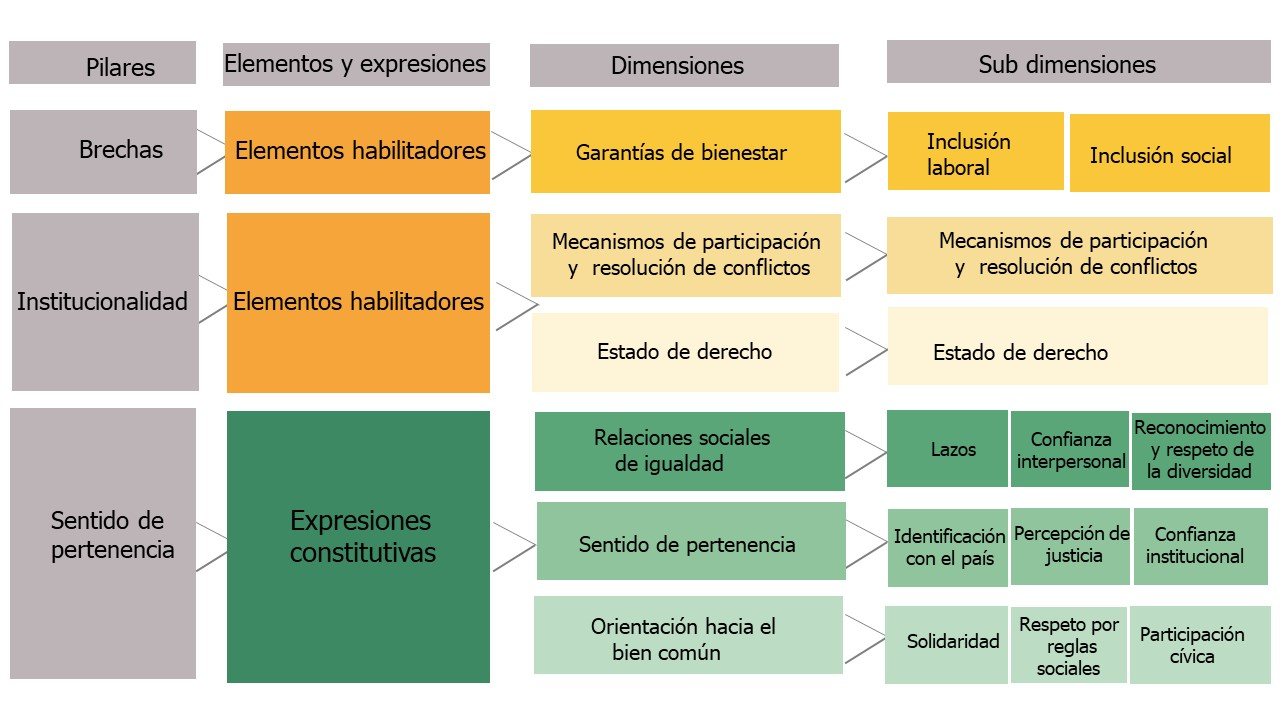
\includegraphics[width=1\linewidth,height=1\textheight]{images/dimensiones-cepal} 

}

\caption{Resumen dimensiones CEPAL.}\label{fig:esquema-cepal}
\end{figure}

El modelo de cohesión social de la CEPAL se caracteriza por ser de naturaleza \textbf{multidimensional}, es decir, se asume que la cohesión social no se puede reducir a una única dimensión ni medición, sino que debe ser abordado considerando distintos componentes o dimensiones. La investigación más actual sobre cohesión social asume esta perspectiva y en gran medida coincide con las dimensiones identificadas por CEPAL, como son relaciones sociales de igualdad, sentido de pertenencia y orientación hacia el bien común (\protect\hyperlink{ref-schiefer_essentials_2016}{Schiefer \& Noll, 2016}). Este tipo de modelos multidimensionales también se caracterizan por el establecimiento de subdimensiones e indicadores para cada uno de ellos, que es el objetivo principal de este primer capítulo.

\emph{Datos}

En este capítulo y los siguientes se utilizaran los daos de la encuesta \href{https://coes.cl/encuesta-panel/}{\textbf{ELSOC} (Estudio Longitudinal Social de Chile)} que se asocien al contenido de cada una de las dimensiones y subdimensiones del concepto de cohesión social. La selección de esta encuesta para este estudio se basa no solamente en la presencia de indicadores de cohesión social, sino también es que permitirá analizar cambios anuales de \textbf{trayectorias individuales} en dimensiones y subdimensiones de cohesión social entre 2016 y 2020. Dado que en esta encuesta panel se entrevista a las mismas personas año a año (N=3,000 app.), es posible analizar cambios en el tiempo de manera más precisa que mediante la comparación de distintas muestras en distintos momentos (donde no es posible despejar si los cambios en los indicadores se asocian a un momento distinto o a que las personas son distintas).

La encuesta ELSOC es aplicada por medio de un cuestionario estructurado que posee 7 módulos diferentes: Territorio, Redes y actitudes sociales, Ciudadanía y democracia, Desigualdad y legitimidad, Conflicto social, Salud y bienestar y Caracterización sociodemográfica. Posee un muestreo probabilístico, estratificado (por tamaño de ciudades), por conglomerados y multietápico (aleatorio en todas sus etapas). Para esta muestra se seleccionaron aleatoriamente 40 ciudades con más de 10.000 habitantes (92 comunas de 13 regiones), dentro de estas se escogieron aleatoriamente 1067 manzanas. Dentro de cada manzana se escogieron hogares aleatoriamente y dentro de cada hogar fueron elegidos también de manera aleatoria personas de 18 años o más. Por lo tanto, su unidad básica de observación son personas individuales. Asimismo, la población objetivo son hombres y mujeres de 18 a 75 años. Esta encuesta alcanza un 77\% de representatividad de la población total del país y un 93\% de la población urbana, con un error muestral del 2\%. La muestra alcanzada en 2019 posee las respuestas de 3417 individuos, que incluye respuestas de participantes de la primera ola (2016) y de la muestra de refresco iniciada en 2018 (\protect\hyperlink{ref-coes_radiografia_2019}{COES, 2019}) \{\textgreater\textgreater actualizar a 2020\textless\textless\}.

Para la selección de items de la encuesta se privilegiarán aquellos que se repiten en las distintas versiones (olas) de la encuesta, de manera de permitir la comparación en el tiempo. Dentro de estos items repetidos existen algunos que se repiten de manera intercalada (cada dos años), que se utilizarán en caso de requerir mayor información para las subdimensiones de cohesión social. Los análisis de selección de items para este capítulo se realizarán con los items de la ola 2016, y en el caso de items intercalados que aparezan desde el 2017 se utilizarán los correspondientes a ese año.

\emph{Sobre medición de dimensiones y subdimensiones}

Dado que la encuesta ELSOC no fue diseñada específicamente en base al modelo de cohesión de CEPAL, en este capítulo se identificarán aquellos items que se relacionan más cercanamente a cada uno de los conceptos presentes en las subdimensiones. Para ello también se tomará como referencia la propuesta de items elaborad por la CEPAL basada en encuestas comparativas de América Latina. Luego de esta identificación se procederá a un análisis descriptivo y de asociaciones entre los items que conforman cada subdimension, y en base a ello se realizará una propuesta de medición de subdimensiones en base a indicadores.

Antes de comenzar con el trabajo de análisis de subdimensiones e indicadores, es pertinente hacer algunos alcances sobre lo que vamos a entender por \emph{medición}. En este contexto, medición hace referencia a otorgar propiedades numéricas a ciertos atributos individuales en base a ciertas reglas. Este proceso por definición no es exacto y conlleva error, ya que muchos de los conceptos que se trabajan en ciencias sociales no se pueden medir directamente y se consideran por lo tanto constructos latentes (como clase, estatus, pertenencia, confianza, entre muchos otros). Gran parte del trabajo de buscar evidencia de validez de las mediciones se trata justamente de poder cuantificar y minimizar este error. Para esto no solo basta con un análisis de \emph{validez aparente}, referido a que el contenido de los items parezcan relacionarse con el concepto que se desea medir, sino también con las propiedades métricas del indicador, como son la variabilidad y covariabilidad/correlación con otras medidas asociadas. Es por ello que en medición muchas veces se utilizan indicadores múltiples para un mismo concepto - sobre todo aquellos de naturaleza compleja y multidimensional como cohesión social -, de modo de poder identificarlo y estimarlo de una manera más robusta con técnicas específicas de análisis de constructos latentes.

La breve mención a aspectos de medición del párrafo anterior nos permite aclarar el orden y el sentido del análisis que se presenta a continuación. En algunos casos encontraremos items únicos para las subdimensiones, y en este caso no tenemos mayor alternativa que discutir su validez aparente y esperar un bajo nivel de error de medición. En otros casos existen baterías de items múltiples, donde se propondrán indicadores que representen de mejor manera los elementos comunes (covarianza) y que subyacen a la batería, para lo que se utilizarán técnicas de análisis factorial.

Las decisiones respecto de los indicadores de cohesión social variarán según sea el número de items presentes por subdimension:

\begin{itemize}
\item
  1 item: se considerará simplemente el puntaje de la variable.
\item
  2 items: se analizará la correlación entre ambas y sobre esta base se podrá proponer un promedio simple.
\item
  3 items: se analizará la matriz de correlaciones y el alfa de Cronbach como medida de consistencia interna que permita trabajar con el promedio de los items. Esta medida otorga un número que va entre 0 y 1, donde el nivel convencional para considerar consistencia es 0.7 o mayor.
\item
  4 items o más: se realizará un análisis factorial exploratorio para evaluar la dimensionalidad subyacente a los items, y en base a este análisis se realizará un promedio con los indicadores correspondientes a el/los factor(es) que mejor representen la variabilidad subyacente.
\end{itemize}

A continuación se presenta el análisis ordenado por dimensiones y subdimensiones:

\begin{itemize}
\tightlist
\item
  Dimensión relaciones sociales de igualdad:

  \begin{itemize}
  \tightlist
  \item
    lazos
  \item
    confianza interpersonal
  \item
    reconocimiento y respecto de la diversidad
  \end{itemize}
\item
  Dimensión sentido de pertenencia:

  \begin{itemize}
  \tightlist
  \item
    identificación con el país
  \item
    percepción de justicia
  \item
    confianza institucional
  \end{itemize}
\item
  Dimensión orientación hacia el bien común:

  \begin{itemize}
  \tightlist
  \item
    solidaridad
  \item
    respeto por reglas sociales
  \item
    participación cívica
  \end{itemize}
\end{itemize}

Por ejemplo, considerando en primer lugar la dimensión ``Relaciones Sociales de Igualdad'', comenzaremos con la subdimensión ``lazos'' identificando items de la encuesta que representen este concepto, y con la información disponible elaboraremos una propuesta para cubrir cada una de las subdimensiones.

Estas tres dimensiones provienen desde el modelo presentado por la CEPAL, que centra su atención en el nivel nacional y que utiliza fuentes de datos que permiten una comparabilidad entre países. Ya que en este caso estamos utilizando una encuesta nacional, no deja de ser relevante abordar una dimensión territorial que permita complementar y enriquecer el análisis a nivel de país. Por lo tanto, además de las dimensiones del modelo de la CEPAL, de manera exploratoria se agrega una cuarta dimensión de cohesión social en el territorio, que se asocia a la confianza en vecinos, identificación barrial, sociabilidad barrial y satisfacción residencial.

\hypertarget{relaciones-sociales-de-igualdad}{%
\section{Relaciones sociales de igualdad}\label{relaciones-sociales-de-igualdad}}

De acuerdo a la CEPAL, ``esta parte de la definición de la cohesión social se acerca a aquellas que conciben la cohesión social como el compromiso y habilidad para trabajar juntos, incluso cuando los valores que poseen las personas sean distintos (Comisión Económica para África, 2016; Pornschlegel y Jürgensen, 2019; Dragolov y otros, 2013; De Beer, 2014; Woolcock, 2011; Banco Mundial, 2012, 2000; Stanley, 2003). Supone asimismo el principio de reconocimiento recíproco como precondición de la cohesión social (véase, por ejemplo, Jenson, 1998), así como la superación de todas las formas de discriminación'' (\protect\hyperlink{ref-cepal_cohesion_2021}{CEPAL, 2021, p. 45}). Las subdimensiones que componen esta dimesión son lazos, confianza interpersonal y reconocimiento de la diversidad.

\textbf{Lazos}

Según CEPAL (\protect\hyperlink{ref-cepal_cohesion_2021}{2021}), ``Los lazos sociales permiten generar espacios de cooperación que faciliten el desarrollo de relaciones sociales de igualdad, y establece patrones de reciprocidad interpersonal (PNUD, 2013)'' (p.~74)

El indicador utilizado en la propuesta regional de la CEPAL para esta subdimensión es ``importancia de amigos en la vida'', que es un indicador de percepción de la Encuesta Mundial de Valores, a partir del cual se busca cuantificar la intensidad del tejido social en los países de la región. En el caso de ELSOC los items más cercanos a esta operacionalización corresponden a ``Cantidad de amigos/as cercanos'' y ``Tamaño de la red cercana'', que están presentes solo en las olas 2 y 4 de la encuesta. Además, se incluye un item de ``Cantidad de personas que se conocen con diferentes ocupaciones'' (CEO, vendedor ambulante, secretario/a, mecánico de autos, vendedor de tienda, abogado/a, aseador/a de oficina, médico, parvularia, chofer de taxi, camarero/a, contador/a, profesor/a universitario) para poder determinan la heterogeneidad de los lazos; este item está presente en las olas 1, 3 y 5. Un análisis descriptivo de estos items se presenta en la Figura \ref{fig:lazos} y un análisis bivariado en la Figura \ref{fig:lazos-cor}. Estos análisis fueron realizados considerando solo a las personas que participaron en todas las olas mencionadas: el item ``Cantidad de amigos/as cercanos'' utilizado proviene de la ola 2 (n=1886), el item ``Tamaño de la red cercana'' utilizado proviene de la ola 2 (n=1885) y el item ``Cantidad de personas que se conocen con diferentes ocupaciones'' utilizado proviene de la ola 1 (n=1886)

\begin{figure}[H]

{\centering 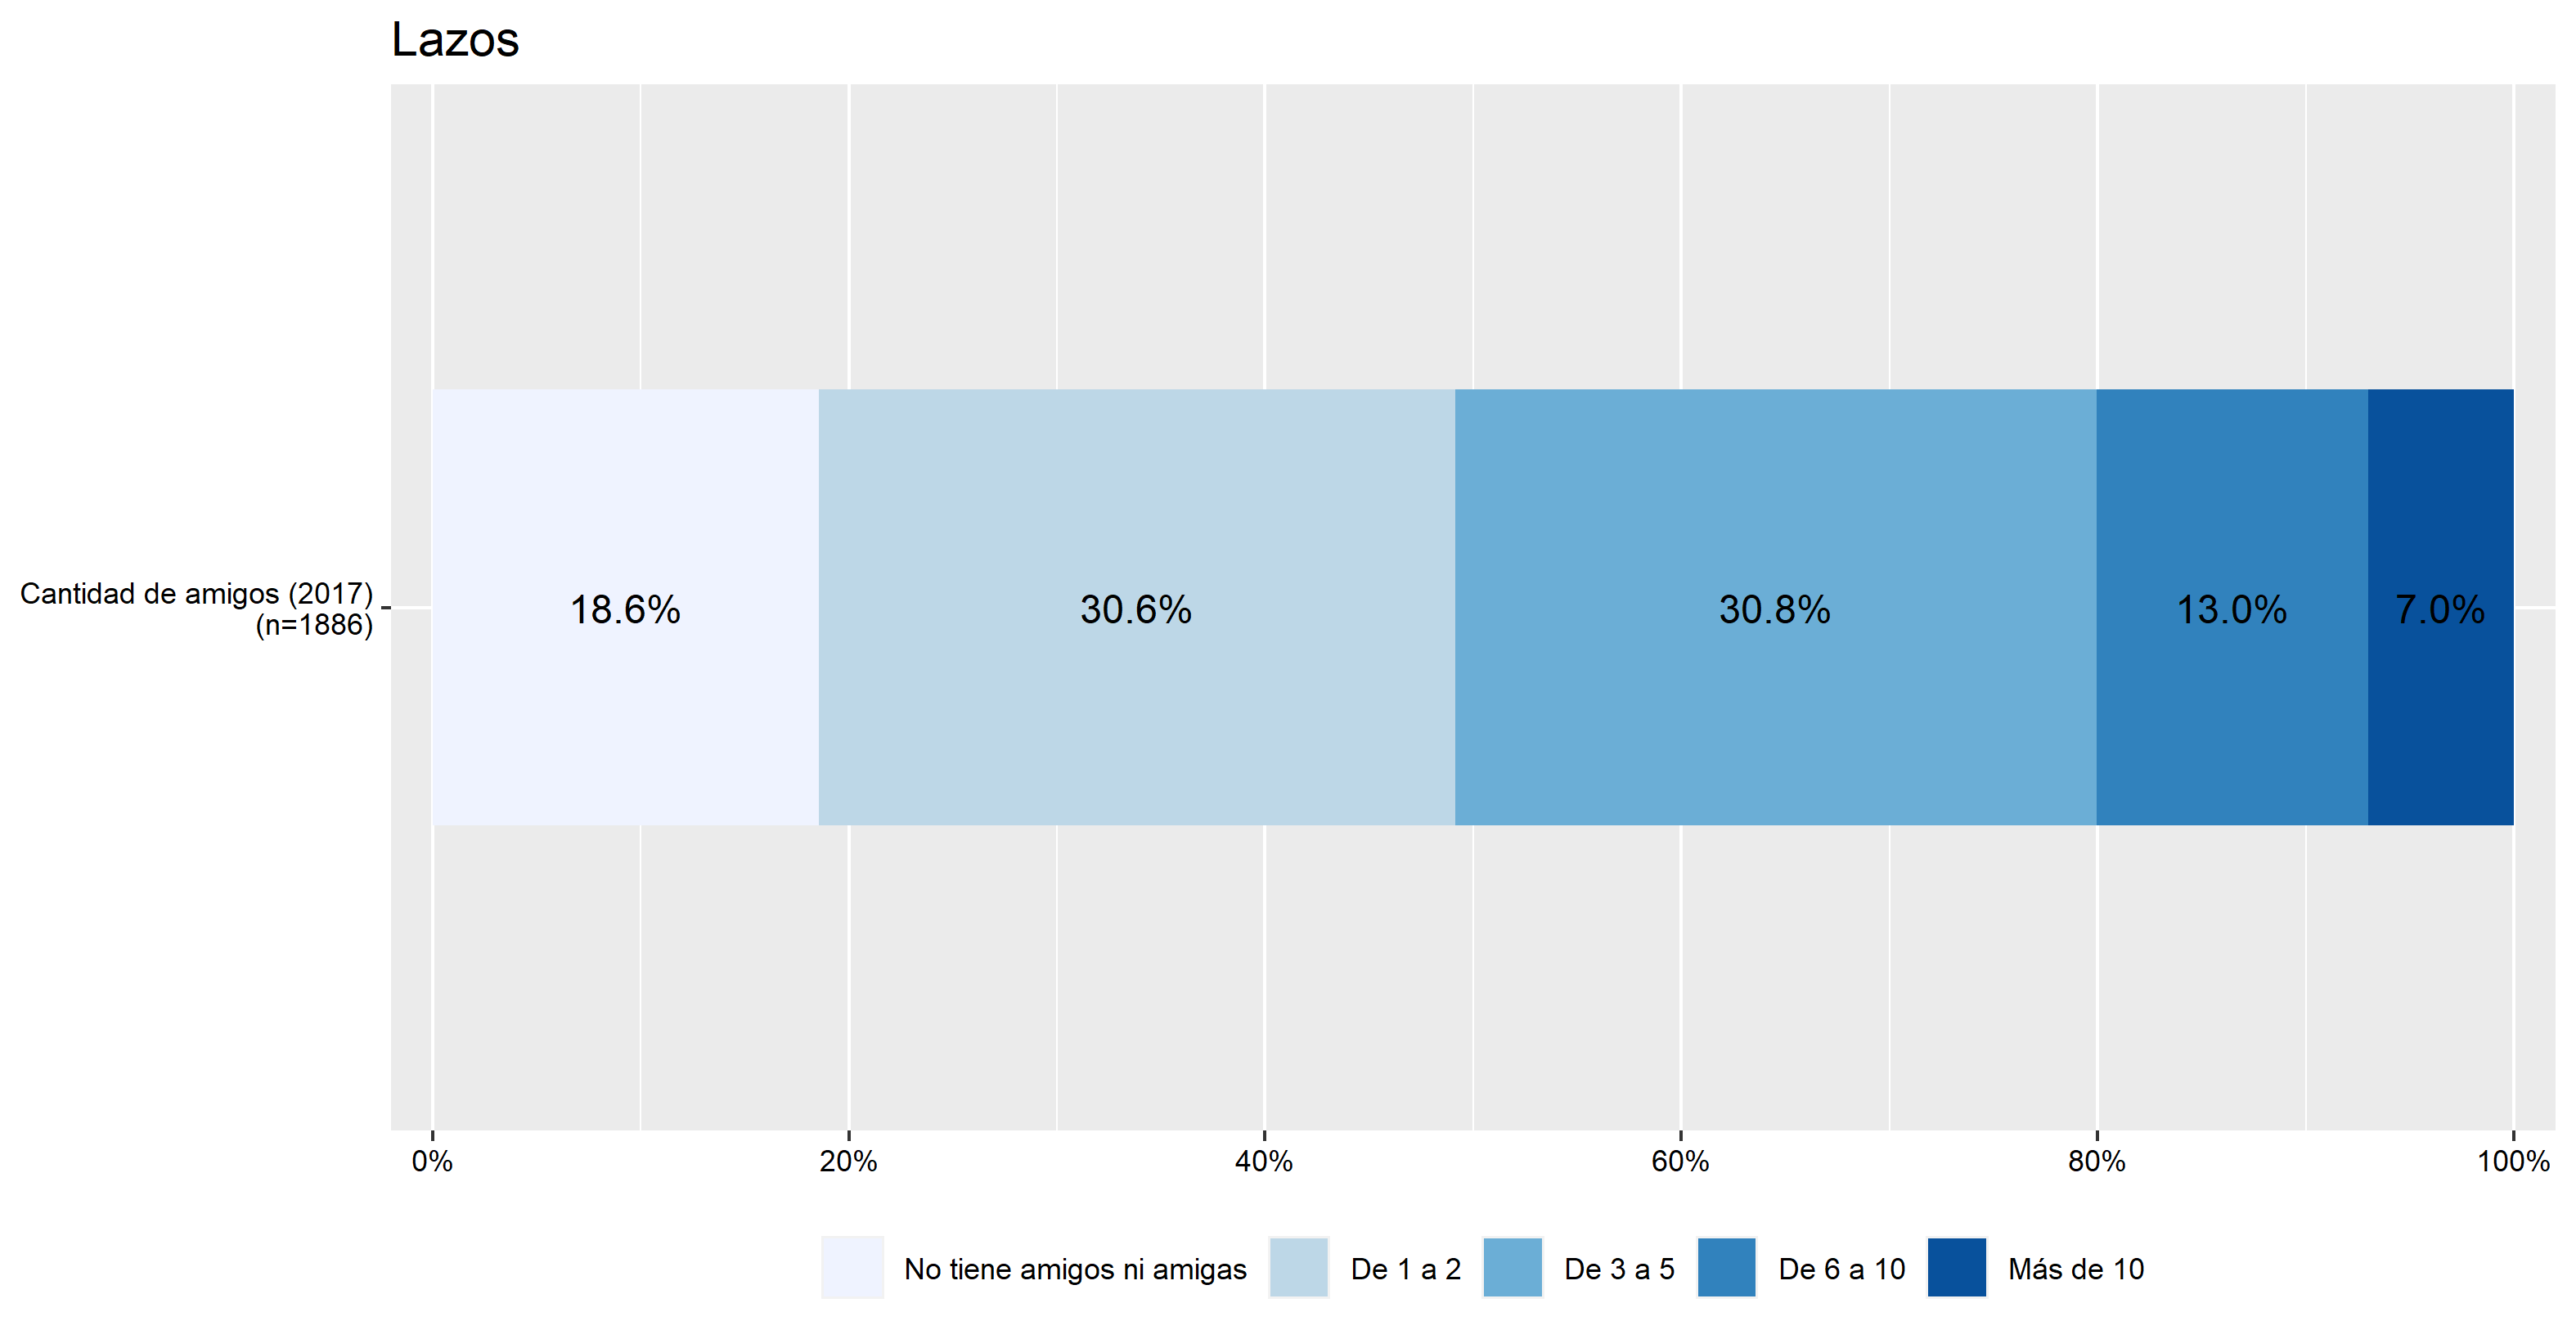
\includegraphics[width=1\linewidth,height=1\textheight]{output/graphs/lazos} 

}

\caption{Lazos.}\label{fig:lazos}
\end{figure}

En la matriz de correlaciones de la Figura \ref{fig:lazos-cor} es posible observar que las correlaciones entre los items están en un rango bajo, donde los items que presentan una correlación mayor son A y C. Para calcular la consistencia interna de estos tres items se utilizó alpha de Cronbach, obteniendo un resultado de 0.36, muy por debajo del valor mínimo recomendado de 0.7. Por lo tanto, para esta subdimensión se considerará un promedio solo de aquellos items que poseen una mayor correlación: ``Cantidad de amigos/as cercanos'' y ``Cantidad de personas que se conocen con diferentes ocupaciones'' (variedad de la red). Ambos indicadores también poseen mayor sentido en el marco de la cohesión social, ya que esta va más allá de la calidad y cantidad de lazos cercanos como familia y amigos, contemplando aquellos lazos sociales más extensos que van más allá de la comunidad cercana.

\begin{figure}[H]

{\centering 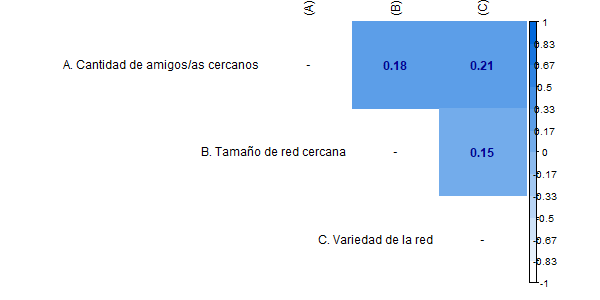
\includegraphics[width=1\linewidth,height=1\textheight]{output/graphs/lazos_cor} 

}

\caption{Asociación de indicadores lazos.}\label{fig:lazos-cor}
\end{figure}

\textbf{Confianza interpersonal}

La confianza interpersonal es un atributo de las relaciones sociales que permite la interacción intergrupal y facilita la acción colectiva a favor de los objetivos compartidos. Por lo tanto, ``la confianza se considera un habilitador de la cooperación y participación (capital social)'' (\protect\hyperlink{ref-cepal_cohesion_2021}{CEPAL, 2021, p. 74}).

En la propuesta regional de CEPAL se utilizan los indicadores ``Confianza en la gente de su comunidad'', que busca cuantificar que tan confiable consideran a los habitantes de su comunidad y ``Confianza en la gente que se conoce por primera vez'', en el cual se cuantifica si se puede confiar en la mayoría de las personas o uno debe ser lo suficientemente cuidadoso con los demás. Al trabajar con ELSOC, los items que van en esta línea son ``Se puede confiar en la mayoría de las personas'', ``La mayoría de las personas tratan de ayudar a las demás'' y ``la mayoría de la gente trata de ser justa'', presentes en las cinco olas. Un análisis descriptivo de estos items (en la primera ola 2016) se presentan en la Figura \ref{fig:confianza-interpersonal} y un análisis bivariado en la Figura \ref{fig:confianza-interpersonal-cor}.

\begin{figure}[H]

{\centering 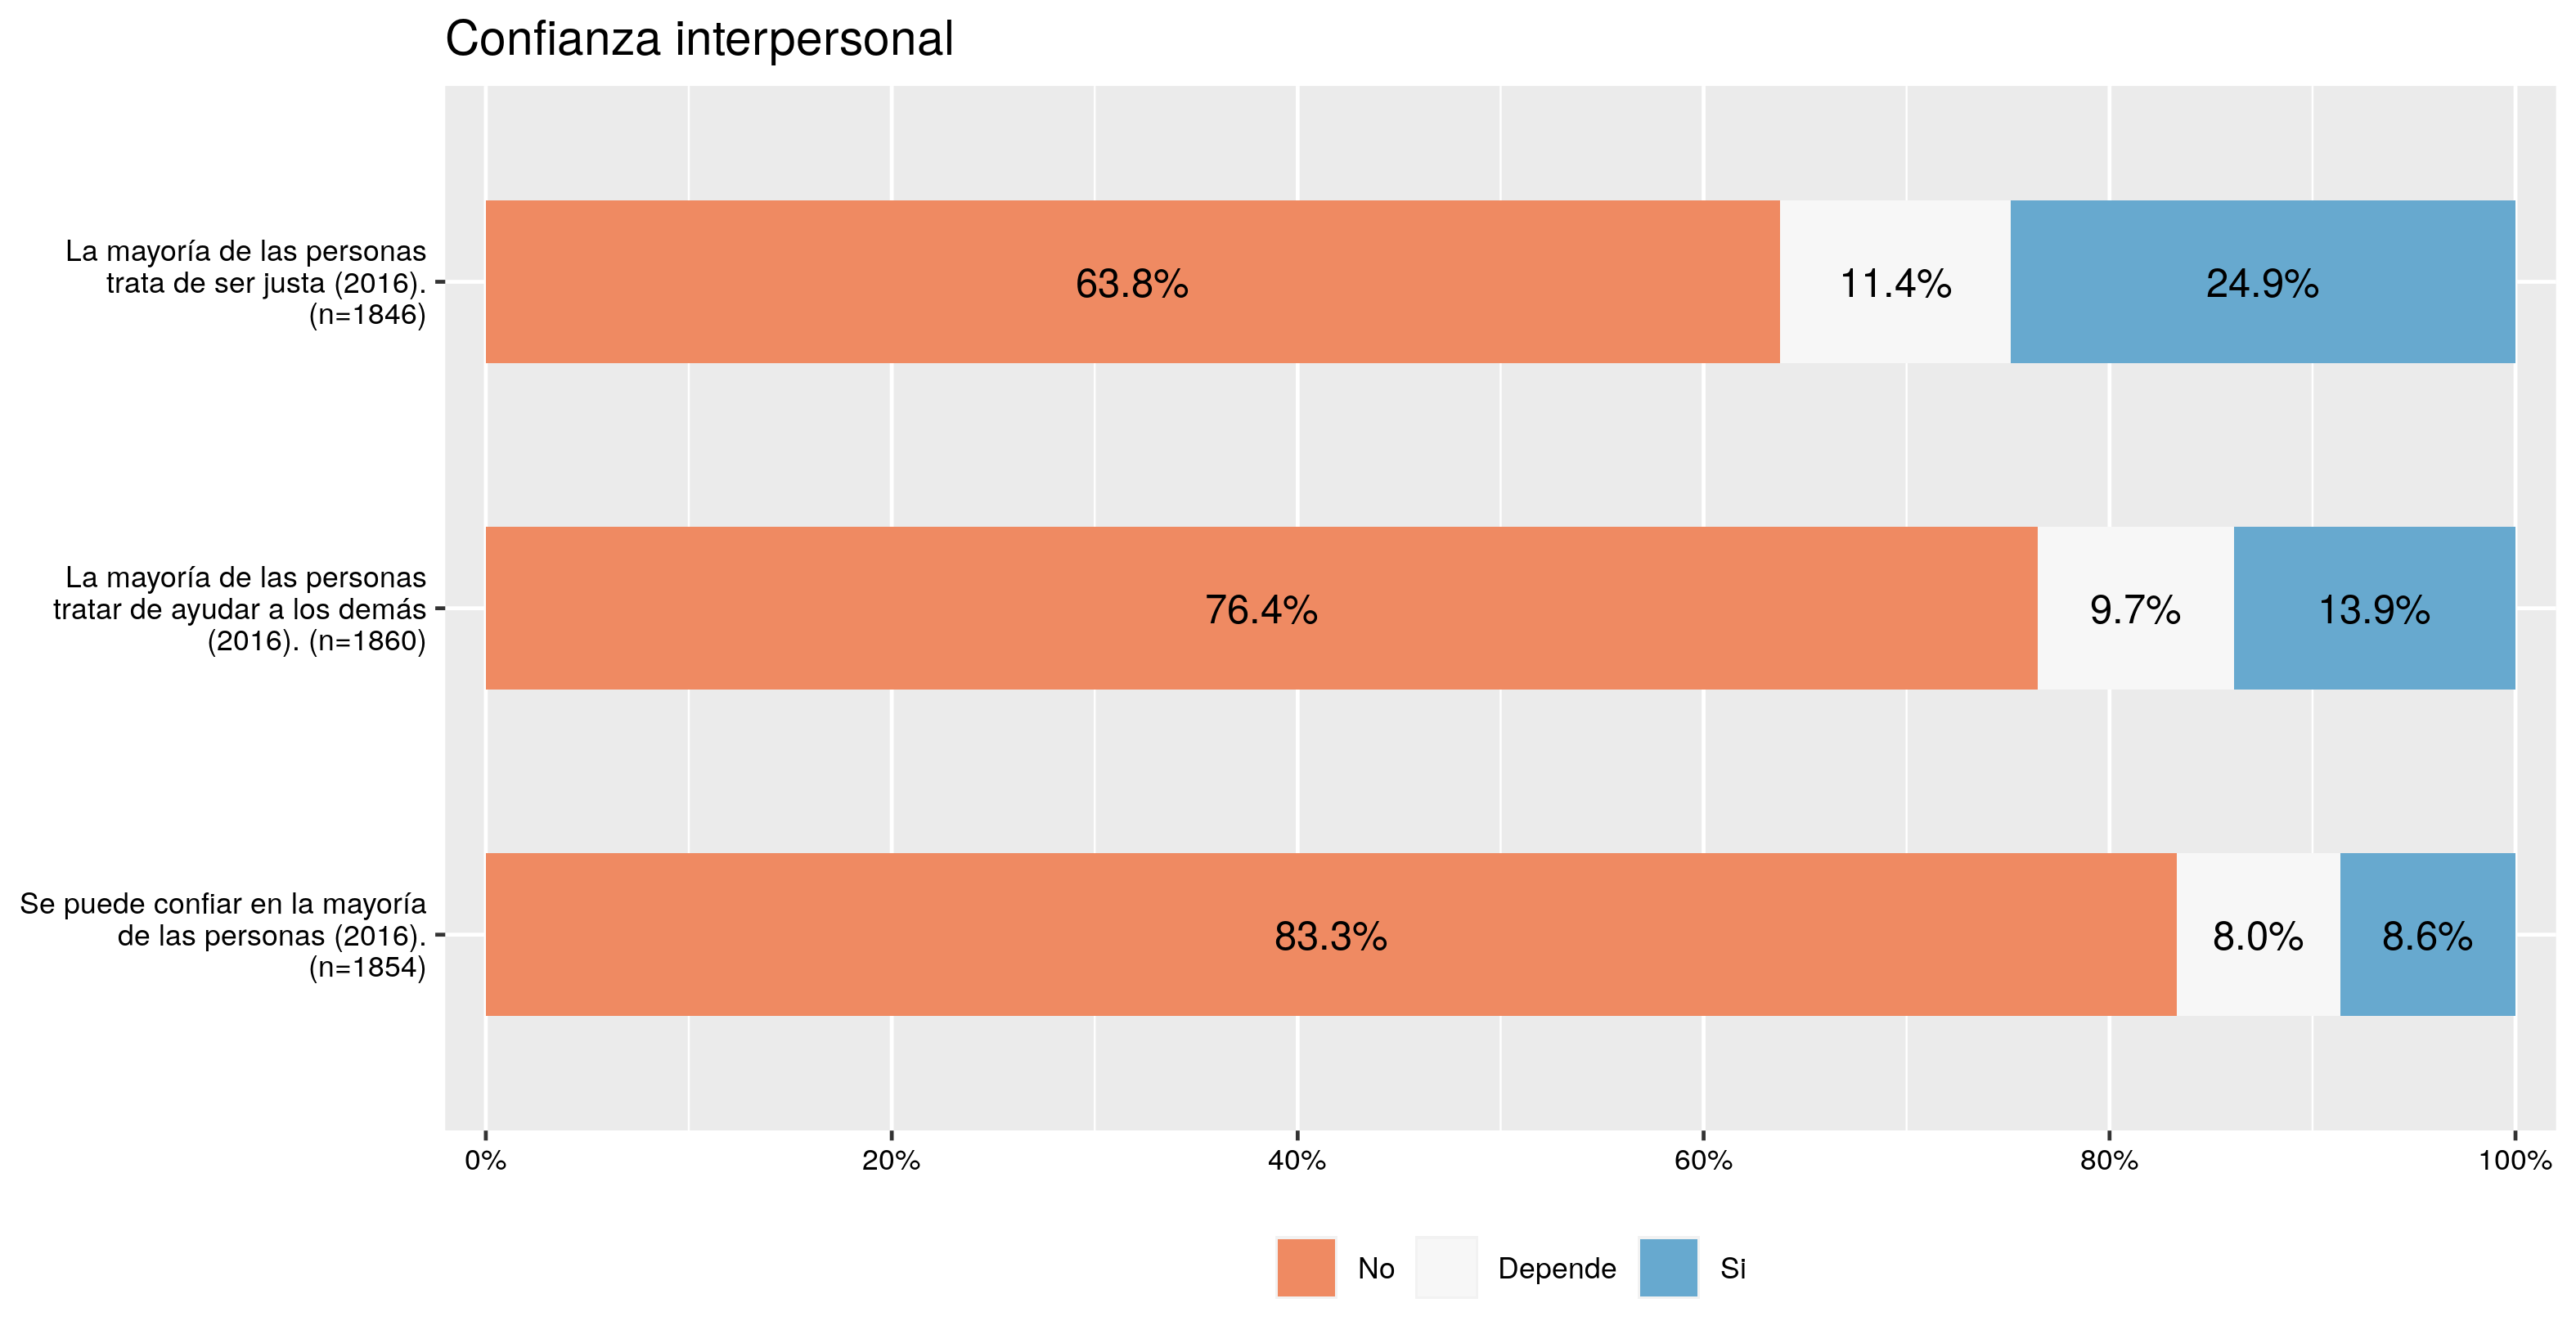
\includegraphics[width=1\linewidth,height=1\textheight]{output/graphs/confianza-interpersonal} 

}

\caption{Confianza interpersonal.}\label{fig:confianza-interpersonal}
\end{figure}

En la matriz de correlaciones de la Figura \ref{fig:confianza-interpersonal-cor} vemos que las correlaciones entre los items van en el rango bajo a moderado, donde los items más correlacionados son A y B. Al calcular la consistencia interna de estos tres items mediante alpha de Cronbach el resultado arroja 0.45, bastante por debajo del límite recomendable de 0.7. Por lo tanto, el índice sugerido para esta subdimensión considera un promedio solo de aquellos items que presentan una correlación mayor: ``Se puede confiar en la mayoría de las personas'' y ``la mayoría de las personas trata de ayudar a los demás''.

\begin{figure}[H]

{\centering 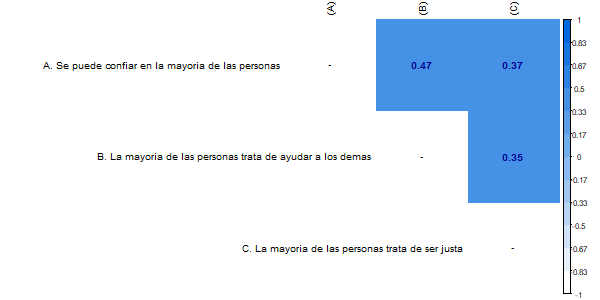
\includegraphics[width=1\linewidth,height=1\textheight]{output/graphs/confianza-interpersonal_cor} 

}

\caption{Asociación indicadores Confianza interpersonal.}\label{fig:confianza-interpersonal-cor}
\end{figure}

\textbf{Reconocimiento y respeto de la diversidad}

Las relaciones sociales de igualdad suponen el reconocimiento de la dignidad del ``otro'' y el reconocimiento de ser parte de una comunidad de iguales en materia de derechos ciudadanos, siendo un elemento que surge de la interacción en redes y asociaciones con individuos de distintas características (\protect\hyperlink{ref-cepal_cohesion_2021}{CEPAL, 2021}).

En la propuesta regional de CEPAL se utilizan dos indicadores en esta subdimensión: ``aprueba el derecho a contraer matrimonio de parejas del mismo sexo'', que se incluye con el objetivo de cuantificar la tolerancia hacia los individuos y comunidades con distinta orientación sexual y ``Los hombres no tienen prioridad sobre la mujer, a la hora acceder a un trabajo'', que se incluye con el objetivo de cuantificar la cultura de igualdad de género en la sociedad. Además, en esta propuesta regional de la CEPAL se deja como pendiente la construcción de un indicador sobre tolerancia a personas de distinta raza y etnia, así como de percepción de discriminación. En el caso de ELSOC encontramos items distintos pero relacionados con actitudes hacia la diversidad: a) Chile pierde su identidad con la llegada de inmigrantes; b) con la llegada de inmigrantes aumenta el desempleo; c) grado de acuerdo con adopción homoparental; d) grado de confianza con personas homosexuales; e) grado de confianza con personas mapuche; y f) grado de confianza con personas inmigrantes. Los dos primeros items están presentes en las cinco olas, adopción homoparental en olas 3 y 4 y el resto de items en las olas 2 y 4. Un análisis descriptivo de estos items se presentan en la Figura \ref{fig:prejuicios} y en la Figura \ref{fig:diversidad} y un análisis bivariado en la Figura \ref{fig:diversidad-cor}. Estos análisis fueron realizados considerando solo a las personas que participaron en las olas mencionadas: el item ``Chile pierde su identidad con la llegada de inmigrantes'' utilizado proviene de la ola 1 (n=1855), el item ``con la llegada de inmigrantes aumenta el desempleo'' proviene de la ola 1 (n=1854), el item ``grado de acuerdo con adopción homoparental'' proviene de la ola 3 (n=1860), el item ``grado de confianza con personas homosexuales'' proviene de la ola 1 (n=1803), el item ``grado de confianza con personas mapuche'' proviene de la ola 1 (n=1774) y el item ``grado de confianza con personas inmigrantes'' proviene de la ola 1 (n=1757).

\begin{figure}[H]

{\centering 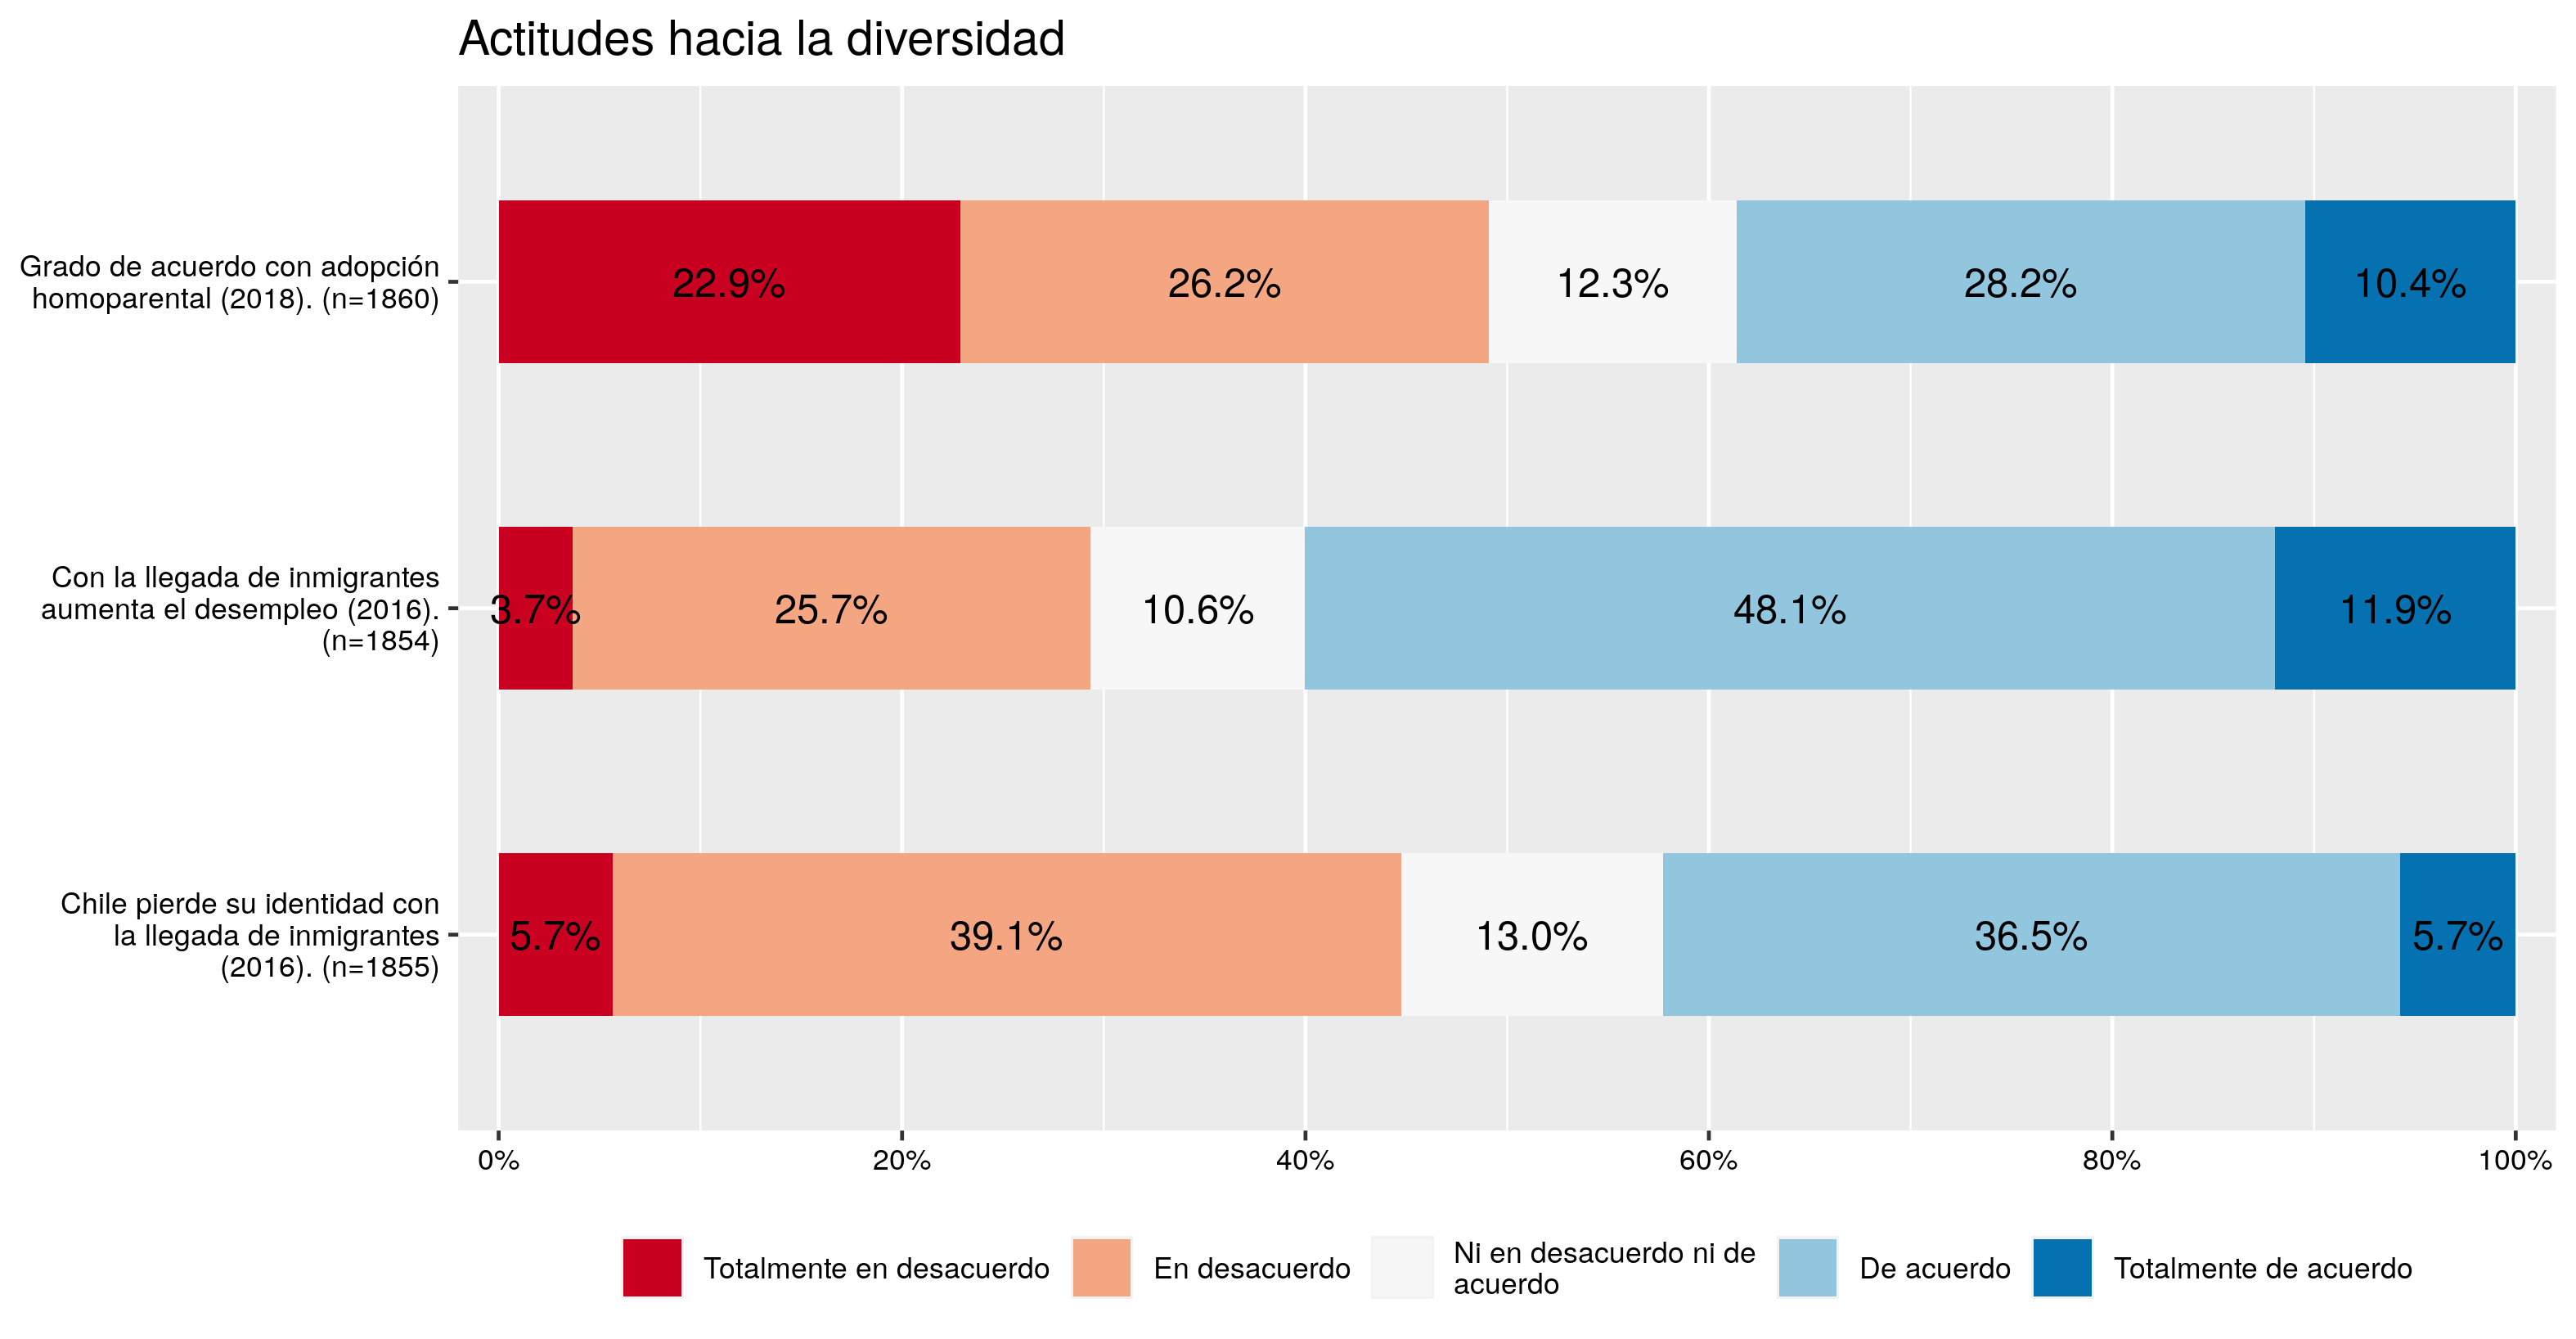
\includegraphics[width=1\linewidth,height=1\textheight]{output/graphs/prejuicios} 

}

\caption{Prejuicios hacia inmigrantes y adopción homoparental.}\label{fig:prejuicios}
\end{figure}

\begin{figure}[H]

{\centering 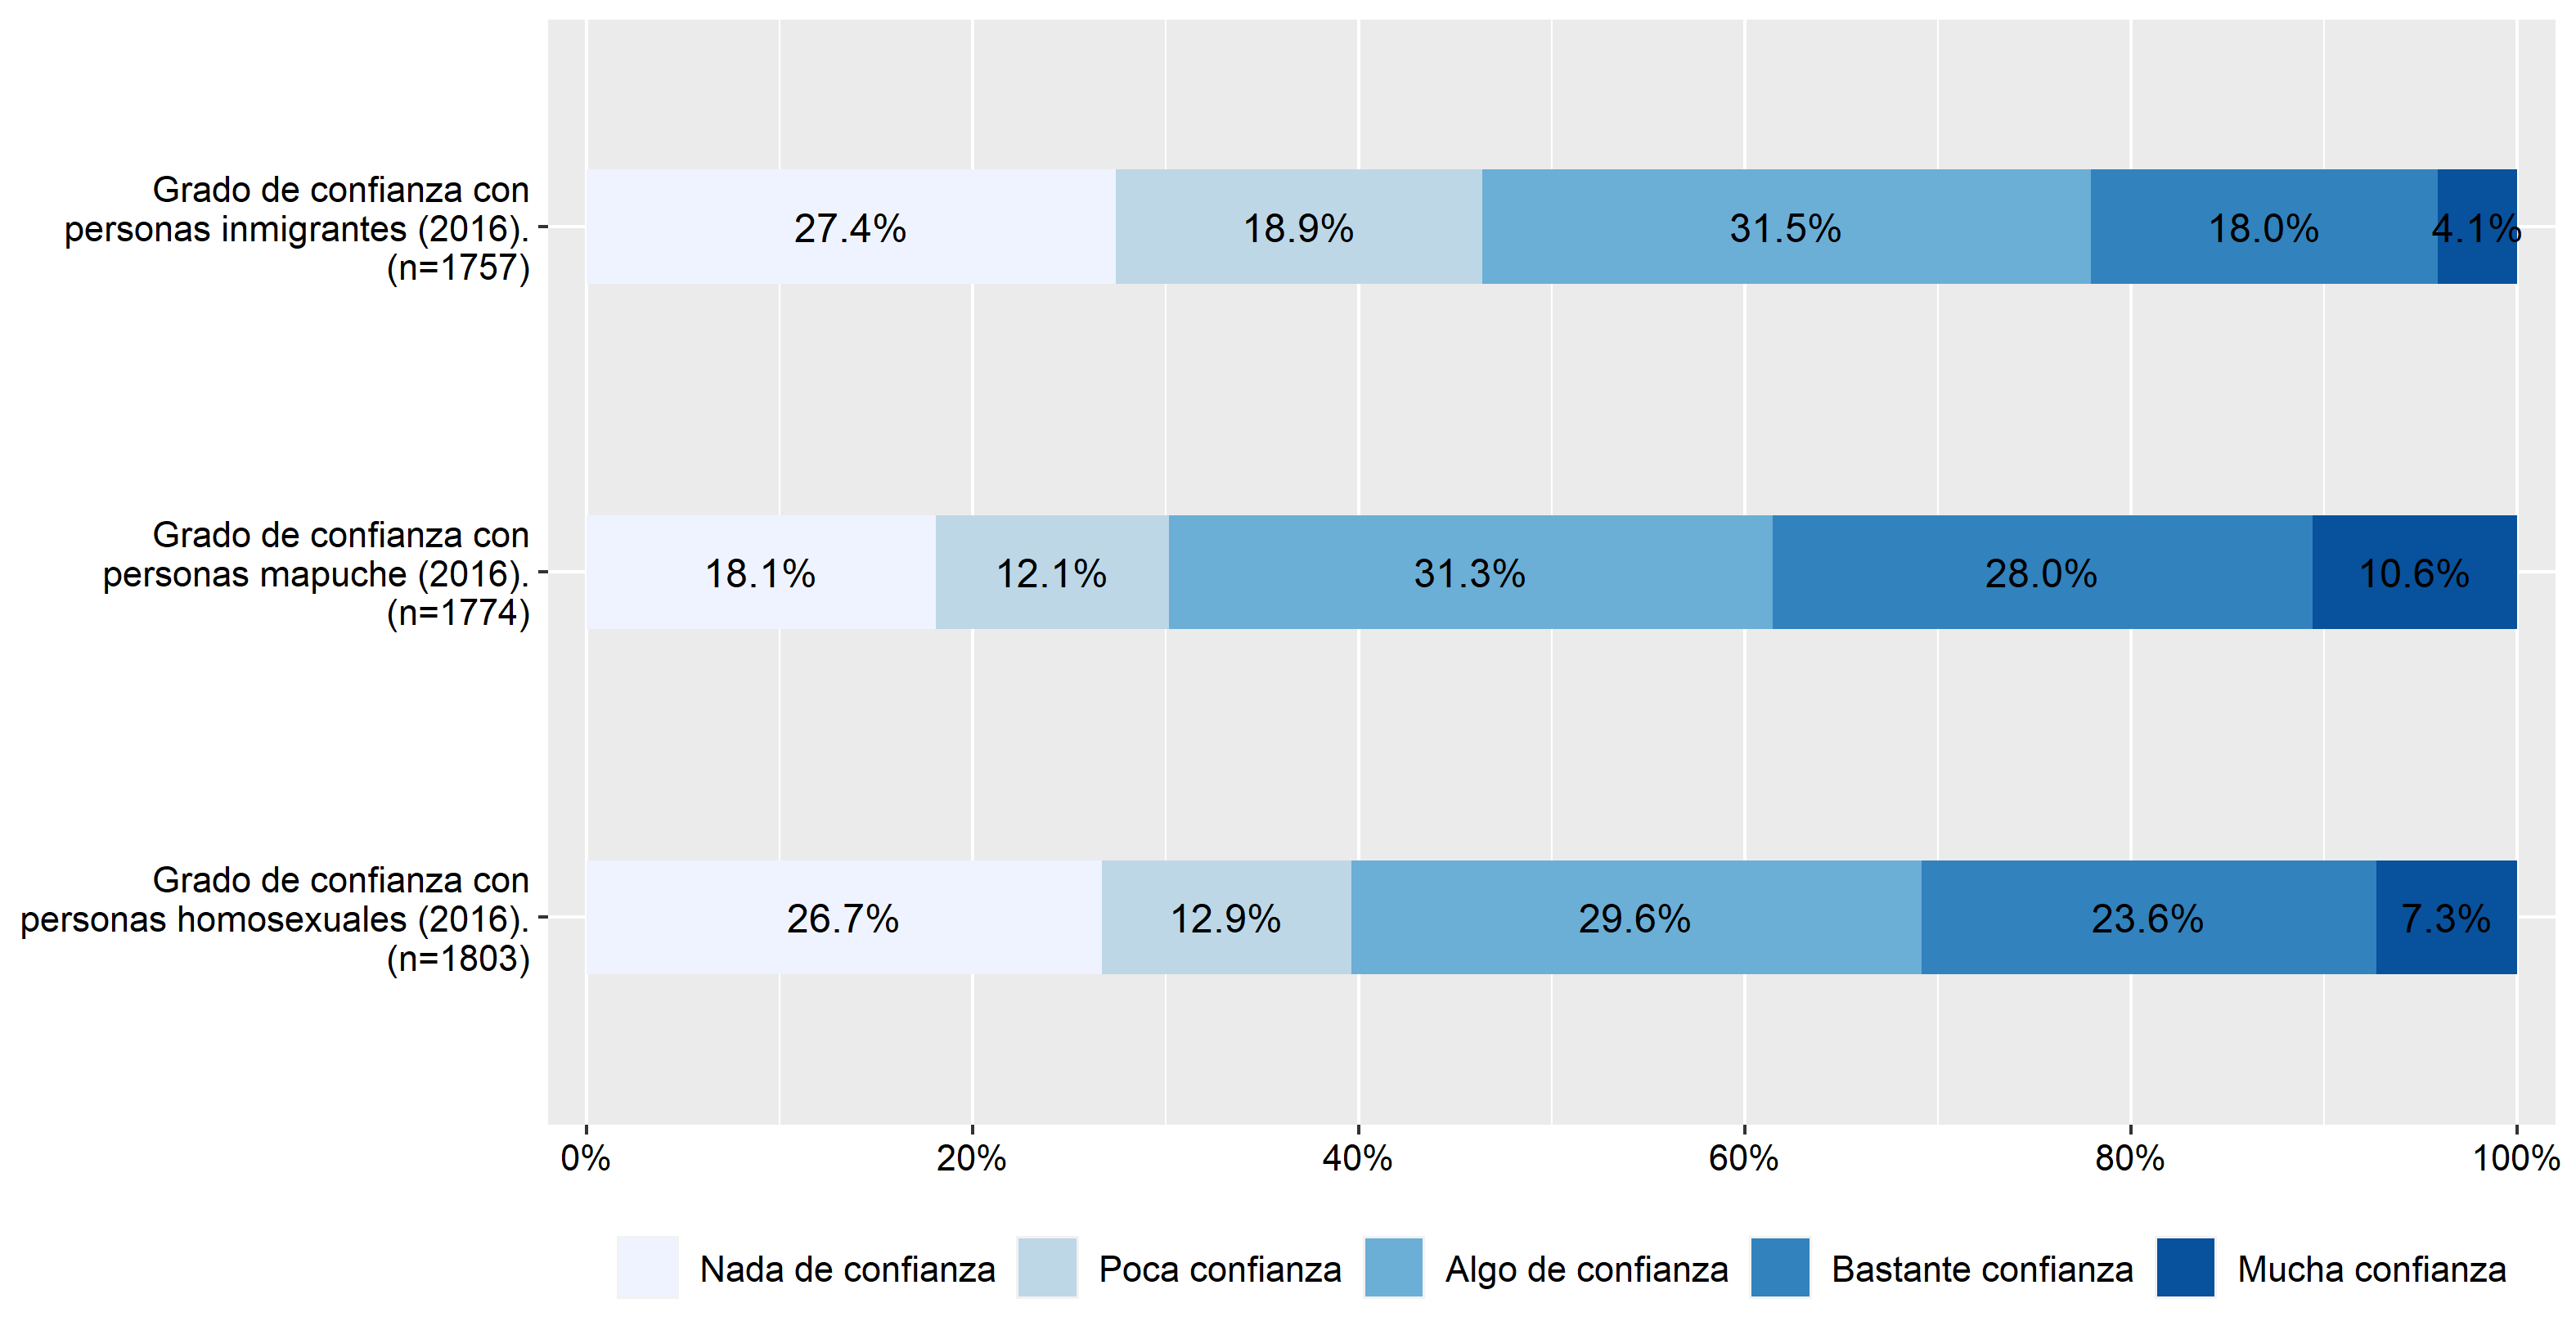
\includegraphics[width=1\linewidth,height=1\textheight]{output/graphs/diversidad} 

}

\caption{Grado de confianza grupos sociales.}\label{fig:diversidad}
\end{figure}

\begin{figure}[H]

{\centering 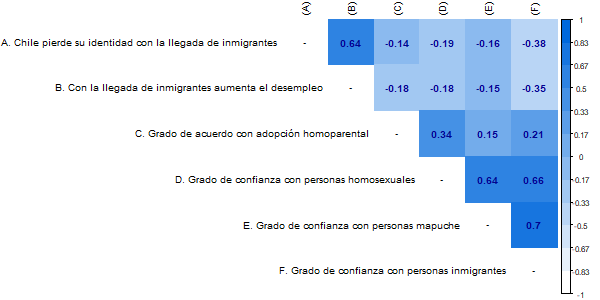
\includegraphics[width=1\linewidth,height=1\textheight]{output/graphs/diversidad_cor} 

}

\caption{Asociación de indicadores de la subdimensión Reconocimiento y respeto de la diversidad.}\label{fig:diversidad-cor}
\end{figure}

Para poder avanzar hacia la construcción de un índice basado en esta serie de items utilizaremos análisis factorial exploratorio, que nos entrega información de las dimensiones comunes que subyacen a un conjunto de items. La Tabla \ref{tab:div-fa} nos muestra el resultado de la extracción de tres factores:

\begin{longtable}[]{@{}l@{}}
\caption{\label{tab:div-fa}Dimensiones de reconocimiento y respeto de la diversidad.}\tabularnewline
\toprule
\endhead

\includegraphics[width=8.33333in,height=\textheight]{output/tables/div_fa.png} \\
\bottomrule
\end{longtable}

En la Tabla \ref{tab:div-fa} observamos en la primera columna los items que se están analizando, y las siguientes columnas que comienzan con ML se refieren a cada uno de los factores extraídos, en este caso tres. Los valores de la tabla en estas columnas nos hablan de la intensidad de la relación entre items y factores en una escala de 0 a 1, donde sobre 0.7 se asume una asociación considerable entre item y factor. La columna \emph{Uniqueness} (unicidad) se refiere a la proporción de varianza que el indicador no comparte con los factores (varianza única), y la fila \emph{Proportion Var} al final de la tabla informa la proporción de la varianza del factor en relación a la varianza total.

Respecto a este análisis en particular, en la segunda columna (ML1) se observa un factor que se relaciona con las preguntas sobre el grado de confianza de la Figura \ref{fig:diversidad}, luego un segundo factor asociado a las preguntas de inmigrantes, y finalmente un tercer factor asociado a la pregunta de adopción homoparental. Atendiendo ahora a la varianza asociada a estos factores, el primer factor representa casi un 30\% de la varianza, el segundo alrededor de 20\% y el tercero muy por debajo con 8\%. Por lo tanto podemos decir que hay mayor consistencia en los dos primeros factores, y entre ellos dos el asociado a confianza hacia la diversidad es el más nítido. Basándose en este análisis es posible proponer utilizar un índice que represente a la subdimensión de reconocimiento y respeto hacia la diversidad que será calculado a partir de un promedio simple entre los indicadores ``Grado de confianza con personas mapuche'', ``Grado de confianza con personas inmigrantes'' y ``Grado de confianza con personas homosexuales''.

A continuación, en la Figura \ref{fig:relaciones-igualdad} se presenta una matriz de correlaciones de los tres indicadores utilizados en la dimensión Relaciones sociales de igualdad.

\begin{figure}[H]

{\centering 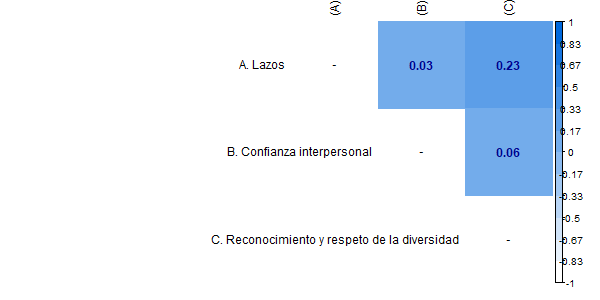
\includegraphics[width=1\linewidth,height=1\textheight]{output/graphs/relaciones_cor} 

}

\caption{Asociación de las subdimensiones de Relaciones sociales de igualdad}\label{fig:relaciones-igualdad}
\end{figure}

\hypertarget{sentido-de-pertenencia}{%
\section{Sentido de pertenencia}\label{sentido-de-pertenencia}}

Una segunda dimensión de la definición propuesta por la CEPAL para cohesión social corresponde al sentido de pertenencia, que ``alude a la vinculación e identificación de las personas respecto a la sociedad y a las instituciones y grupos que los integran. Incluye los niveles micro, meso y macro.'' (\protect\hyperlink{ref-cepal_cohesion_2021}{CEPAL, 2021, p. 45}). Esta definición permite relevar la importancia de ``las dinámicas de reconocimiento y participación social para conducir procesos dinámicos de inclusión que contribuyan a la cohesión social y al logro del bienestar (véase, por ejemplo, Jenson, 1998; Kymlicka, 1998).'' (\protect\hyperlink{ref-cepal_cohesion_2021}{CEPAL, 2021, p. 45}). Las subdimensiones que conforman esta dimensión son identificación con el país, percepción de justicia y confianza institucional.

\textbf{Identificación con el país}

Por medio de esta subdimensión, se busca cuantificar la identificación de los individuos ``con los valores y acciones que representan sus instituciones, y la concordancia con los propios'' (\protect\hyperlink{ref-cepal_cohesion_2021}{CEPAL, 2021, p. 66}).

En la propuesta regional de la CEPAL se incluyen los indicadores ``Orgullo por el sistema político'', que busca medir la adhesión de los encuestados con la labor que realizan sus instituciones en la representación de sus valores y objetivos y ``Orgullo por su nacionalidad'', que busca cuantificar la identificación de los encuestados con los valores y normas que rigen las instituciones del país. Al trabajar con ELSOC se utilizarán los items ``Orgullo de ser chileno'' e ``Identificación con Chile'' que están presentes en las cinco olas. Un análisis descriptivo de estos items se presentan en la Figura \ref{fig:identificacion}. Estos análisis fueron realizados considerando solo a las personas que participaron en las olas mencionadas: el item ``Orgullo de ser chileno'' utilizado proviene de la ola 1 (n=1877) y el item ``Identificación con Chile'' proviene de la ola 1 (n=1880).

La correlación entre estos items es positiva y alta (r=0.76). Por lo tanto, en esta subdimensión se utilizará como índice un promedio simple de ambos items.

\begin{figure}[H]

{\centering 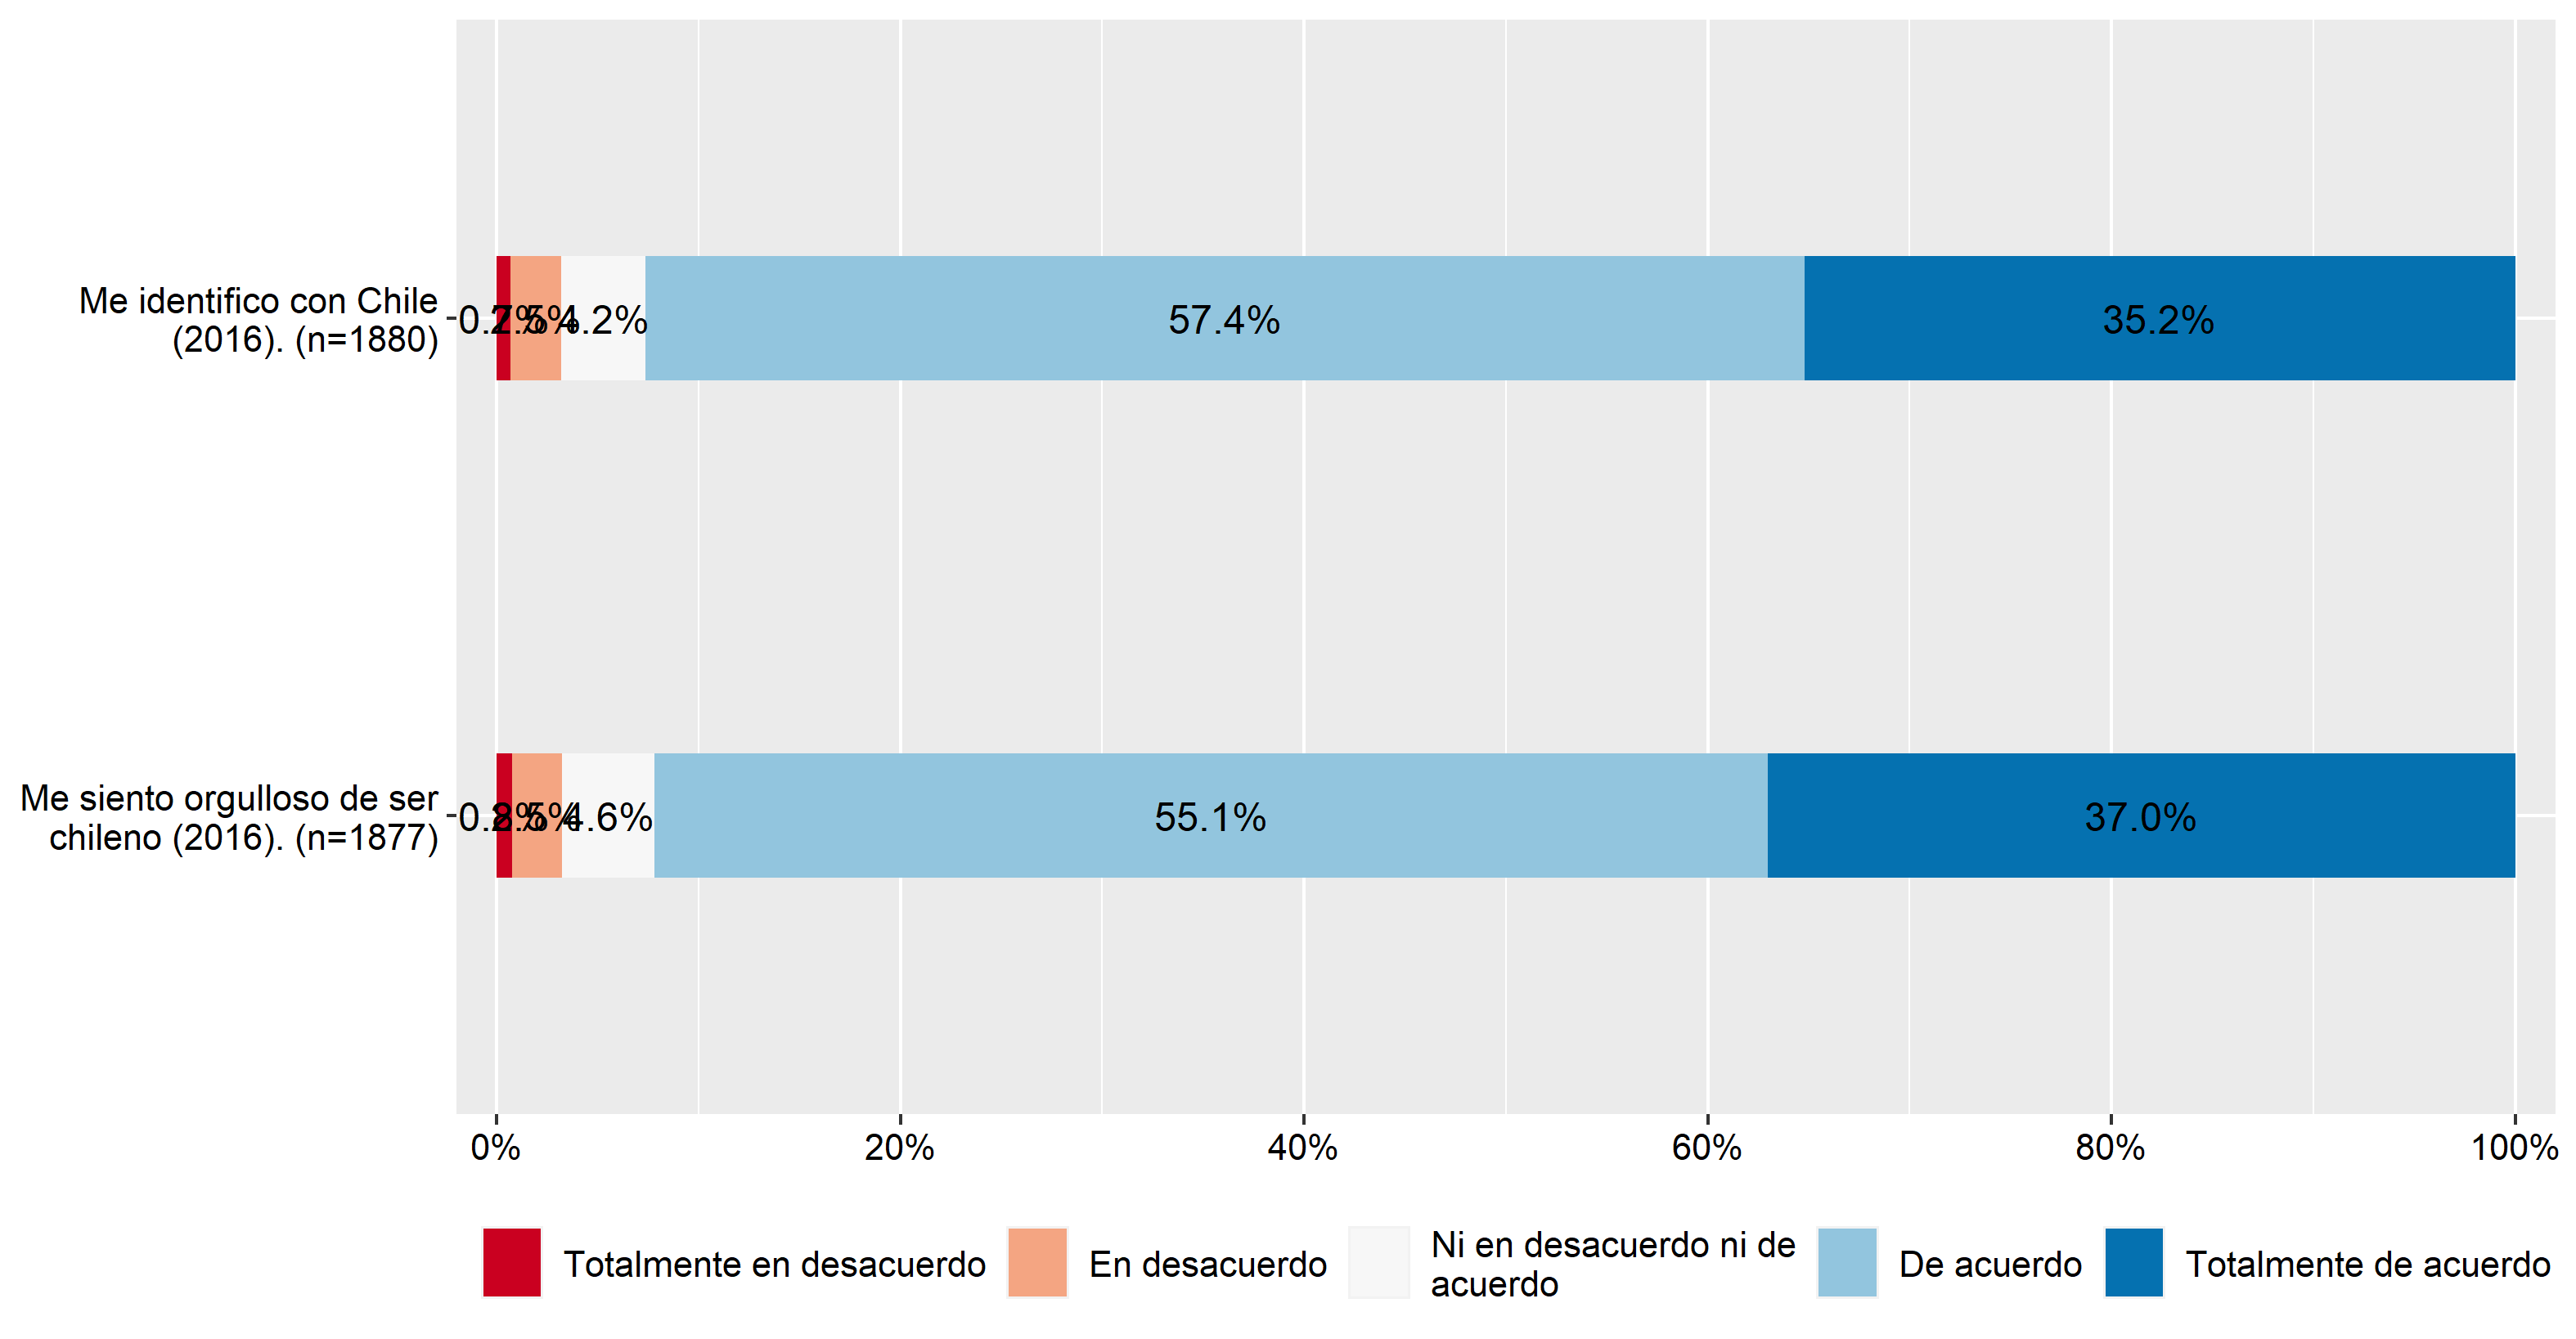
\includegraphics[width=1\linewidth,height=1\textheight]{output/graphs/identificacion} 

}

\caption{Identificación y orgullo con Chile.}\label{fig:identificacion}
\end{figure}

\textbf{Percepción de justicia}

La subdimensión de percepción de justicia refiere al examen que realizan los miembros de la sociedad respecto a la capacidad de las instituciones de entregar bienestar y/o distribuir el poder económico y político (\protect\hyperlink{ref-cepal_cohesion_2021}{CEPAL, 2021}).

En la propuesta regional de la CEPAL se utilizan los indicadores ``Se deben equiparar los sueldos, no mantener desigualdad para incentivar el esfuerzo personal'', que cuantifica percepciones respecto a aversiones hacia la desigualdad; ``El trabajo a largo plazo da beneficios, no las conexiones o suerte'', que busca captar percepciones sobre la estructura de oportunidades en el país y las expectativas de movilidad social; y ``El Estado debe implementar políticas para reducir la desigualdad de ingreso'', que aborda las percepciones respecto a la desigualdad de ingresos en el país. Al trabajar con ELSOC se utilizan los items ``En Chile las personas son recompensadas por su esfuerzo'' y ``En Chile las personas son recompensadas por su inteligencia'', presentes en todas las olas. Un análisis descriptivo de estos items se presentan en la Figura \ref{fig:justicia}. Estos análisis fueron realizados considerando solo a las personas que participaron en las olas mencionadas: el item ``En Chile las personas son recompensadas por su esfuerzo'' utilizado proviene de la ola 1 (n=1878) y el item ``En Chile las personas son recompensadas por su inteligencia'' proviene de la ola 1 (n=1875).

La correlación entre estos items es positiva y alta (r=0.7). Por lo tanto, se utilizará como índice un promedio simple de ambos items en esta subdimensión.

\begin{figure}[H]

{\centering 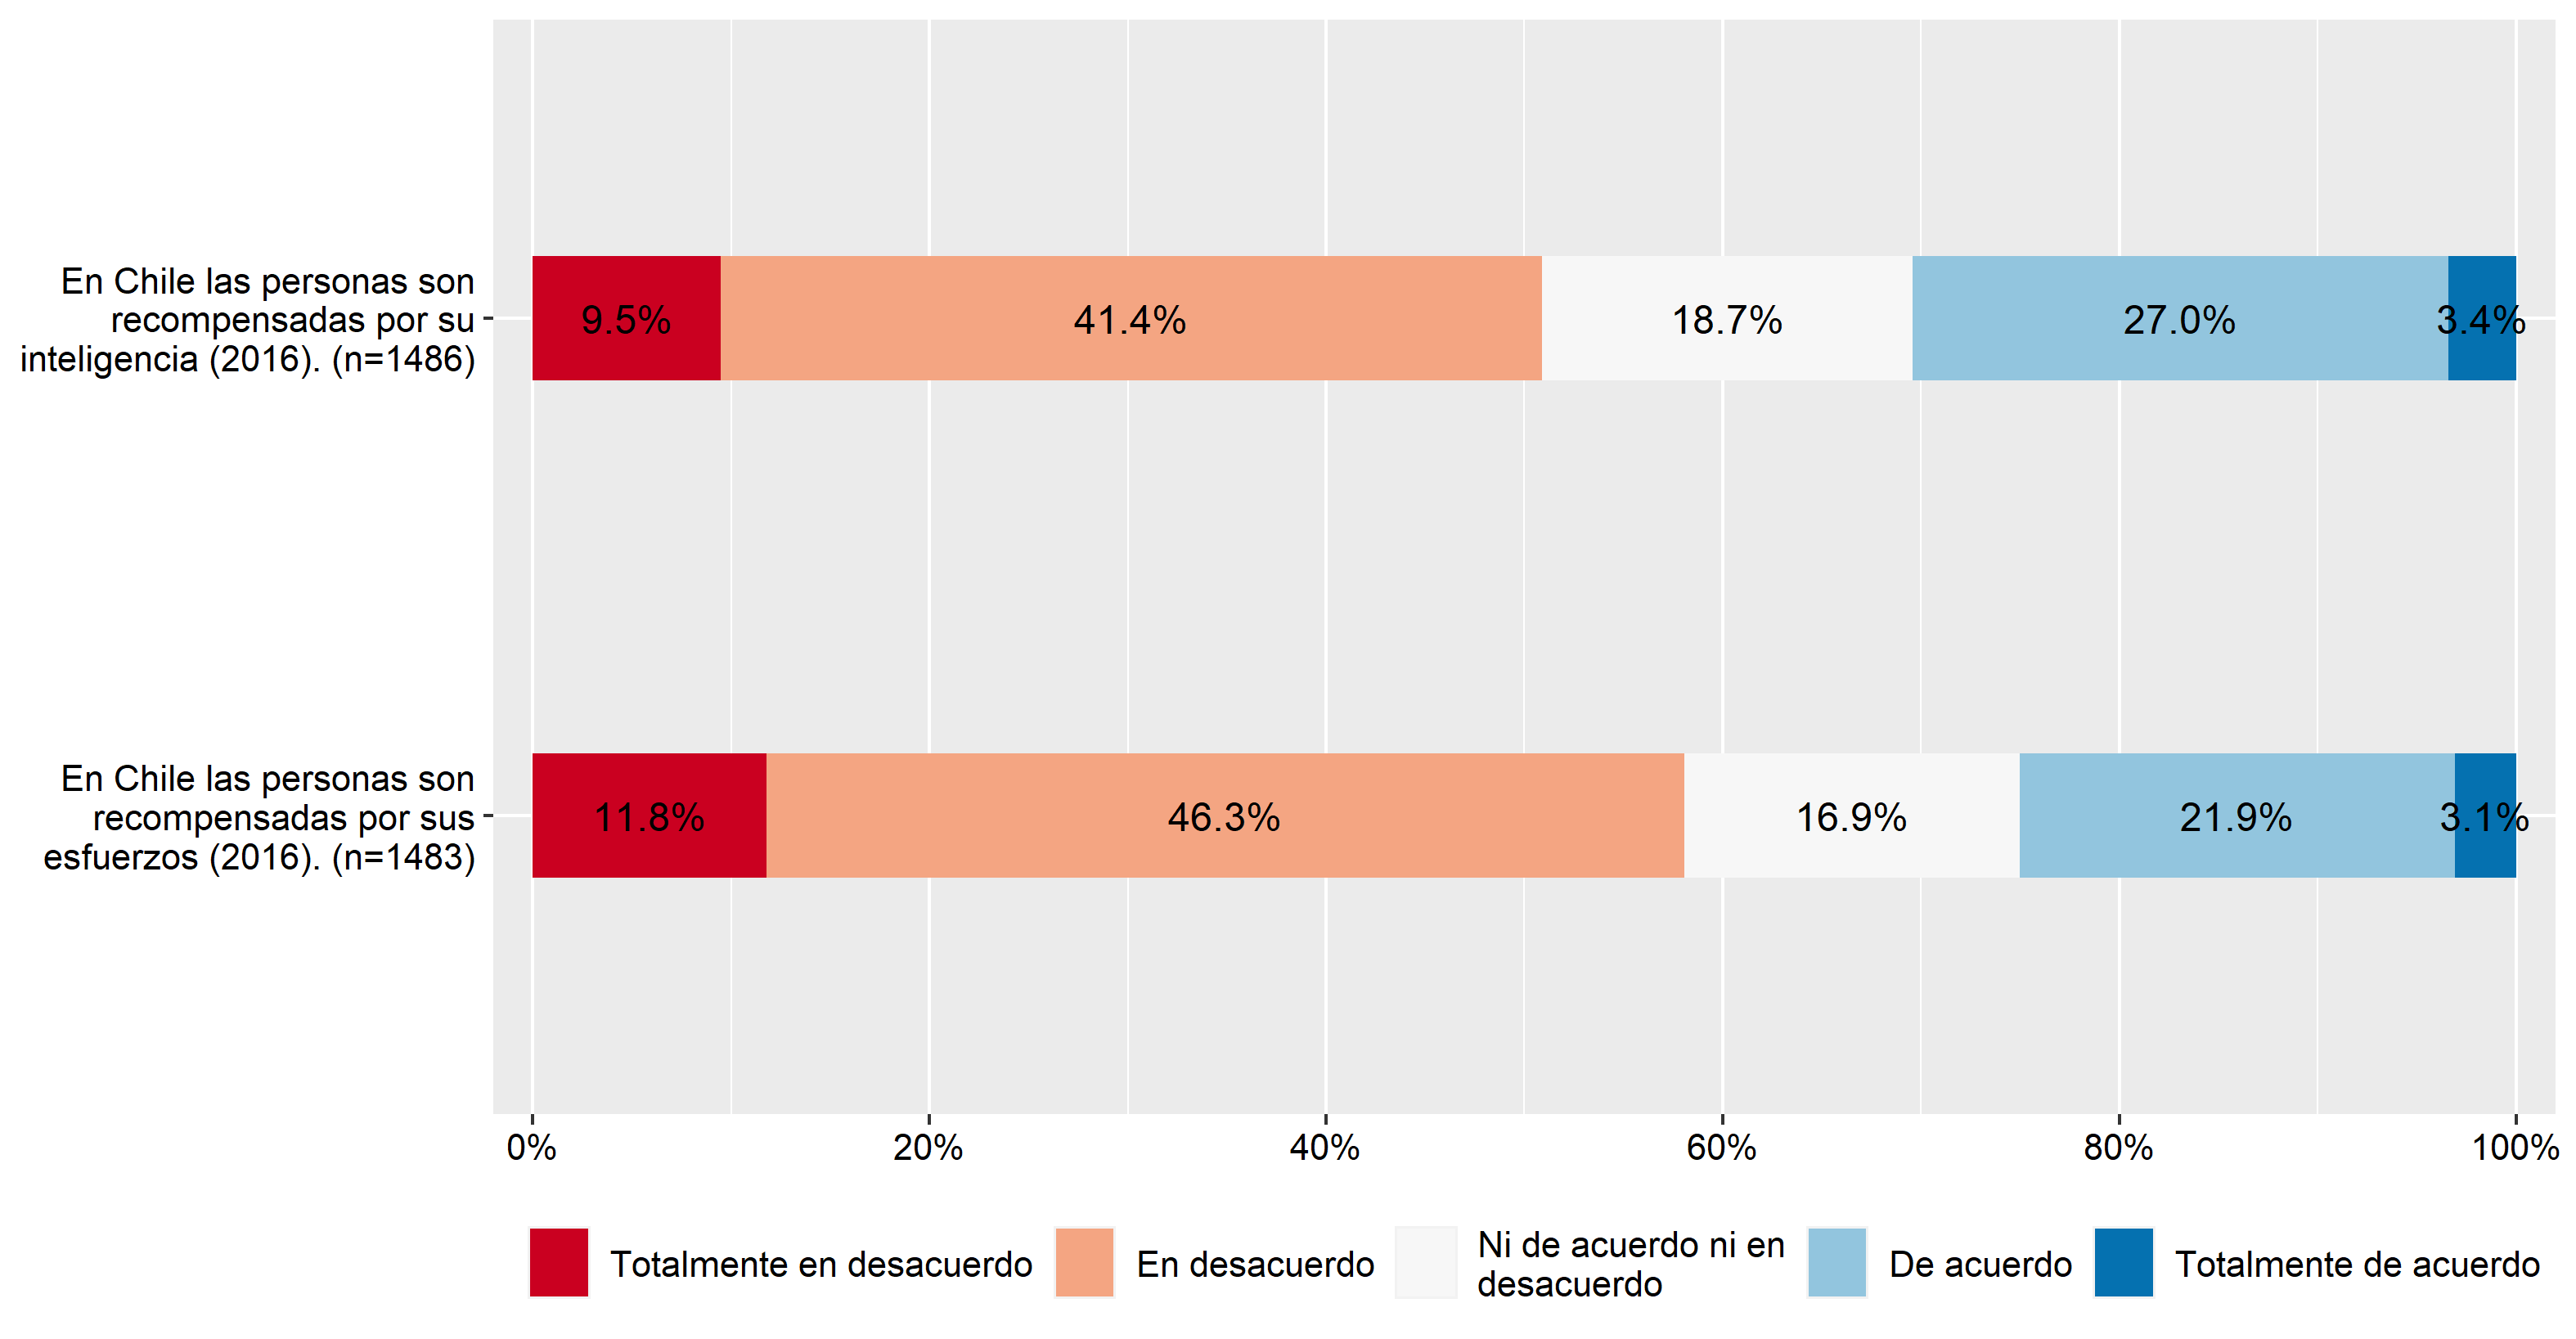
\includegraphics[width=1\linewidth,height=1\textheight]{output/graphs/justicia} 

}

\caption{Descriptivos Percepción de recompensa por esfuerzo e inteligencia.}\label{fig:justicia}
\end{figure}

\textbf{Confianza institucional}

La subdimensión de confianza institucional ``mide la valoración implícita de las acciones llevadas a cabo por las instituciones para representar los valores de la sociedad y/o de orientar la acción hacia el bien colectivo (Warren, 2010)'' (\protect\hyperlink{ref-cepal_cohesion_2021}{CEPAL, 2021, p. 66}).

En la propuesta regional de la CEPAL utilizan grado de confianza en (a) las cortes, (b) el Congreso Nacional, (c) la Policía Nacional, (d) los partidos políticos, (e) el ejecutivo y (f) las elecciones. Al trabajar con ELSOC se utilizan los siguientes ocho items que están presentes en las cinco olas: grado de confianza en (a) el gobierno, (b) los partidos políticos; (c) carabineros; (d) los sindicatos; (e) el poder judicial; (f) las empresas privadas; (g) el congreso nacional; y (h) el presidente/a de la república. Un análisis descriptivo de estos items se presentan en la Figura \ref{fig:confianza-institucional} y un análisis bivariado en la Figura \ref{fig:confianza-institucional-cor}. Estos análisis fueron realizados considerando solo a las personas que participaron en las olas mencionadas: el item grado de confianza en (a) el gobierno proviene de la ola 1 (n=1877), (b) los partidos políticos proviene de la ola 1 (n=1872); (c) carabineros proviene de la ola 1 (n=1884); (d) los sindicatos proviene de la ola 1 (n=1779); (e) el poder judicial proviene de la ola 1 (n=1871); (f) las empresas privadas proviene de la ola 1 (n=1854); (g) el congreso nacional proviene de la ola 1 (n=1856); y (h) el presidente/a de la república proviene de la ola 1 (n=1876).

\begin{figure}[H]

{\centering 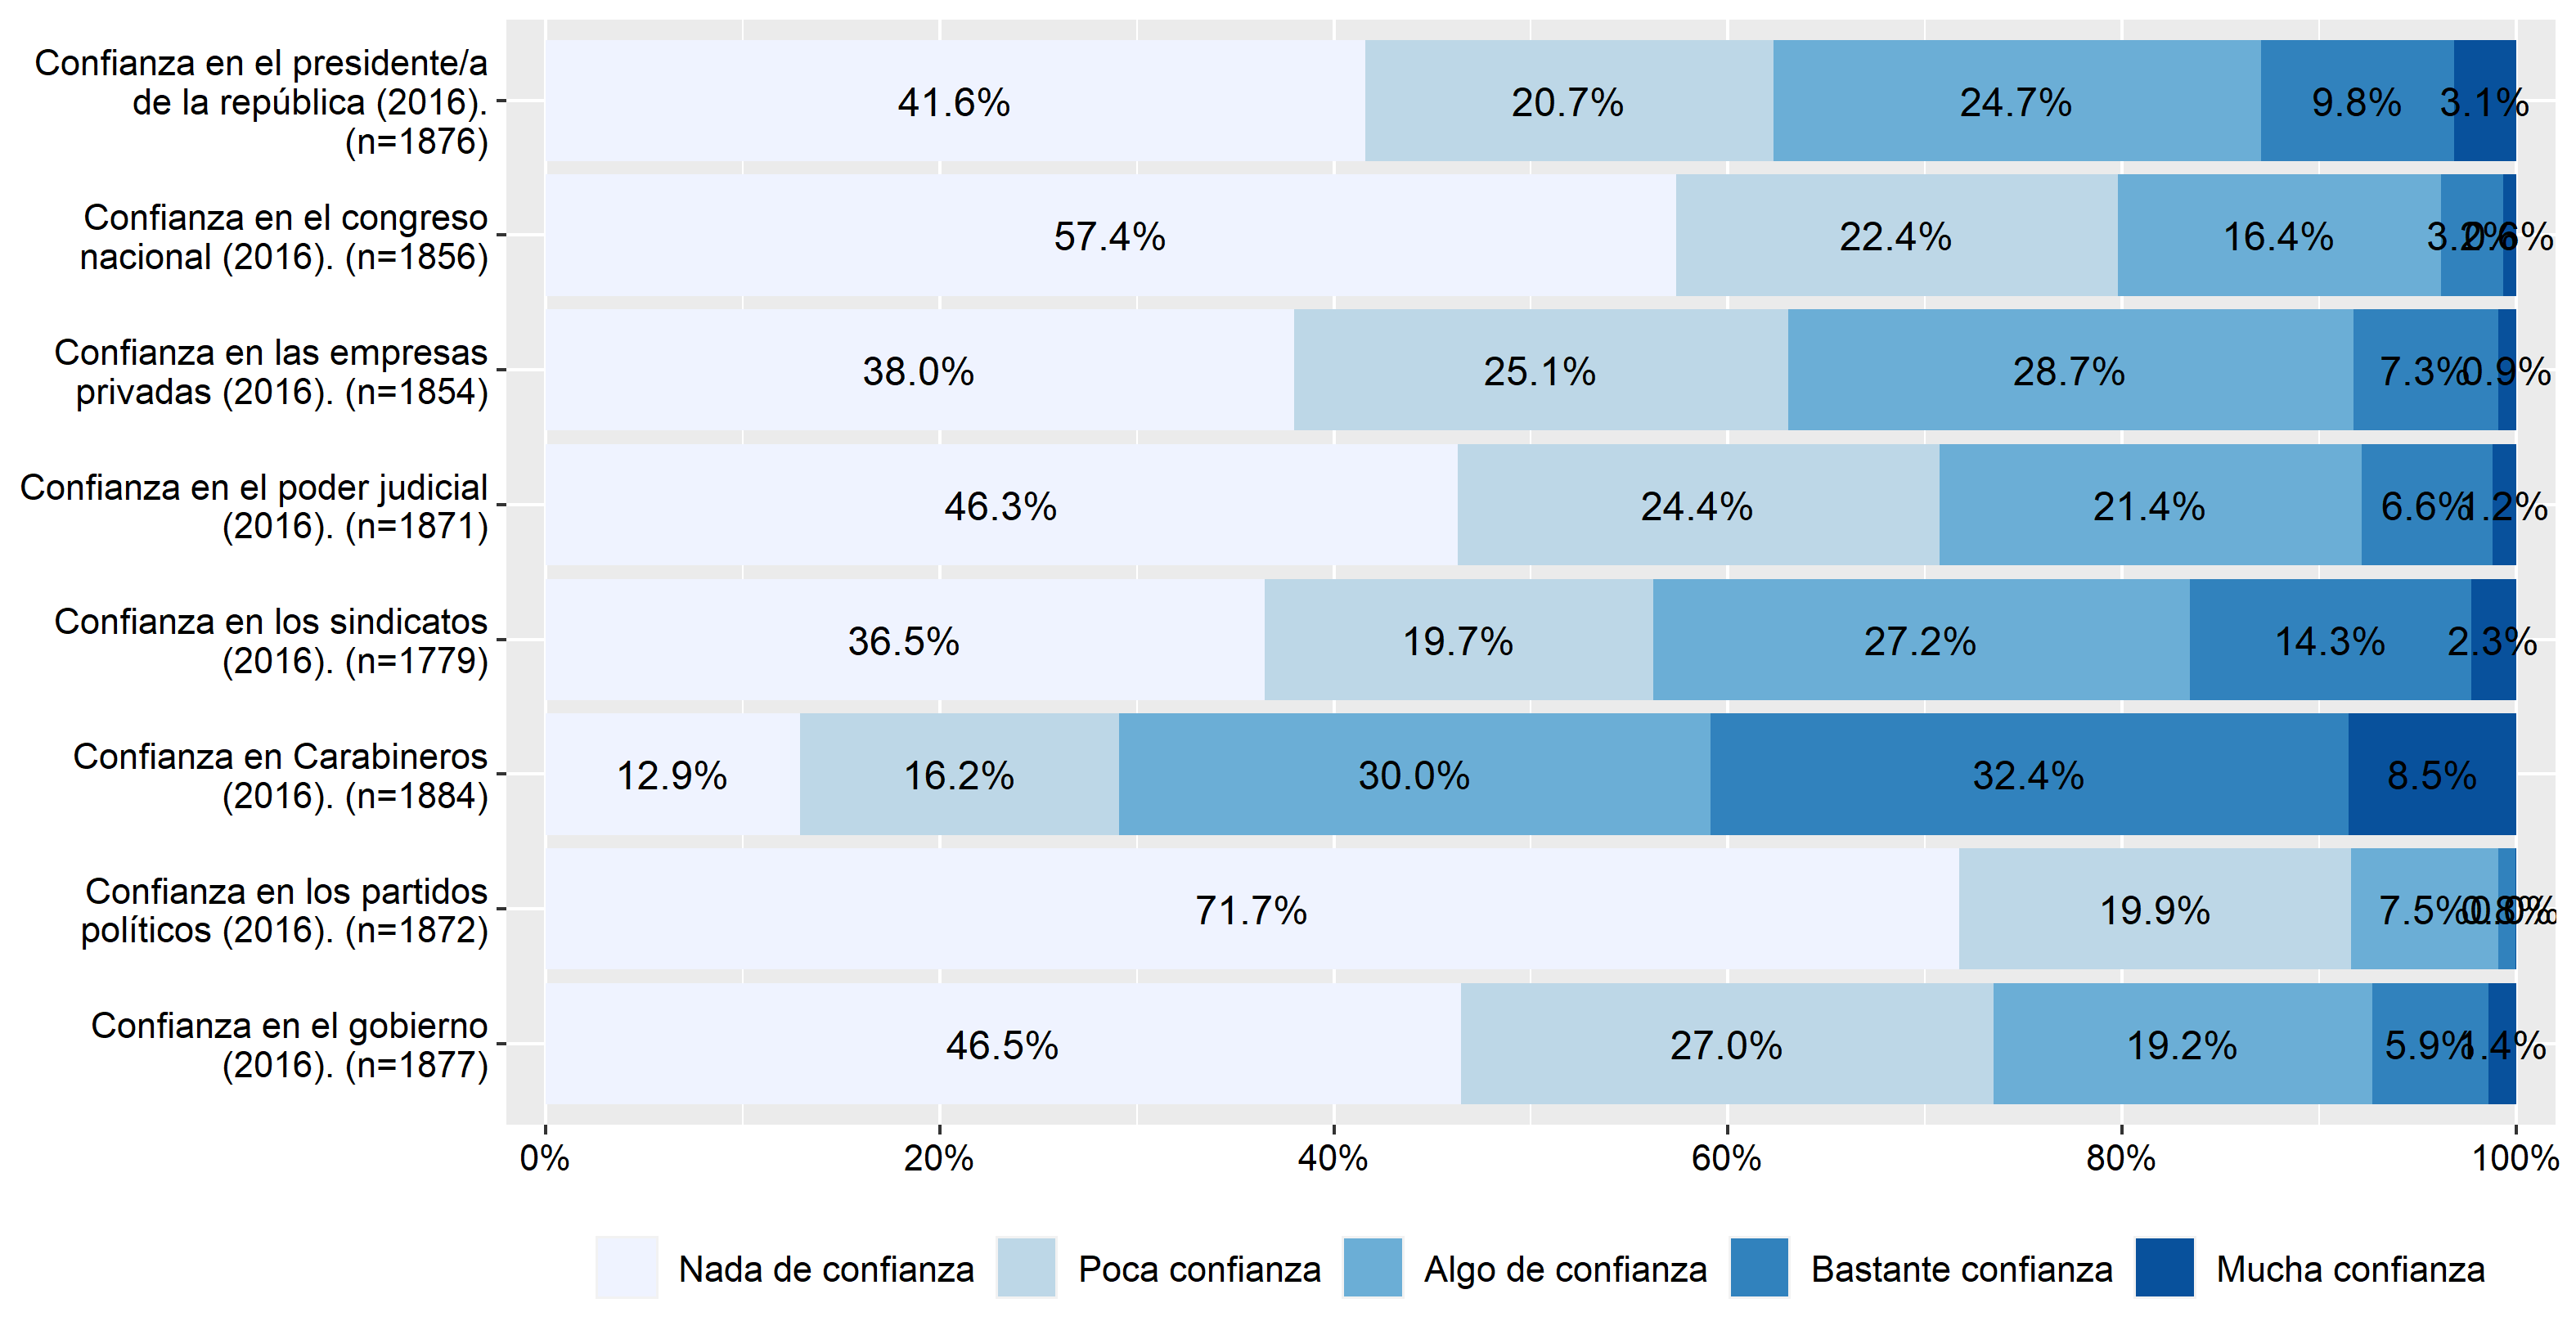
\includegraphics[width=1\linewidth,height=1\textheight]{output/graphs/confianza-institucional} 

}

\caption{Confianza en instituciones.}\label{fig:confianza-institucional}
\end{figure}

\begin{figure}[H]

{\centering 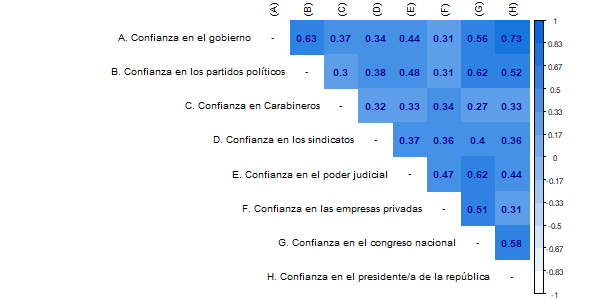
\includegraphics[width=1\linewidth,height=1\textheight]{output/graphs/confianza-institucional_cor} 

}

\caption{Asociación indicadores Confianza institucional.}\label{fig:confianza-institucional-cor}
\end{figure}

En esta oportunidad, nuevamente se utilizó un análisis factorial exploratorio con el objetivo de construir un índice a partir de la información de las dimensiones comunes que subyacen a este conjunto de ocho items. La Tabla \ref{tab:inst-fa} nos muestra el resultado de la extracción de tres factores:

\begin{longtable}[]{@{}l@{}}
\caption{\label{tab:inst-fa}Dimensiones de confianza institucional.}\tabularnewline
\toprule
\endhead

\includegraphics[width=8.33333in,height=\textheight]{output/tables/inst_fa.png} \\
\bottomrule
\end{longtable}

En la Tabla \ref{tab:inst-fa} observamos en la segunda columna (ML2) un factor que se relaciona con las preguntas sobre el grado de confianza con instituciones políticas (el gobierno, presidente/a, partidos políticos), luego un segundo factor (ML3) asociado con instituciones más cercanas a la sociedad civil (empresas privadas, carabineros, sindicatos y poder judicial) y finalmente un tercer factor (ML1) que se asocia con el poder judicial y el congreso. En relación con la varianza asociada a estos tres factores, el primer factor representa un 20\% de la varianza, el segundo un 16\% y el tercero un 15\%. Por lo tanto, existe cierto grado de consistencia en los tres factores, siendo el primero de ellos -relacionado con las instituciones políticas- el que representa una mayor proporción de la varianza y por tanto el índice de confianza institucional incluirá estos tres items.

A continuación, en la Figura \ref{fig:sentido-pertenencia} se presenta una matriz de correlaciones de los tres indicadores utilizados en la dimensión Sentido de pertenencia.

\begin{figure}[H]

{\centering 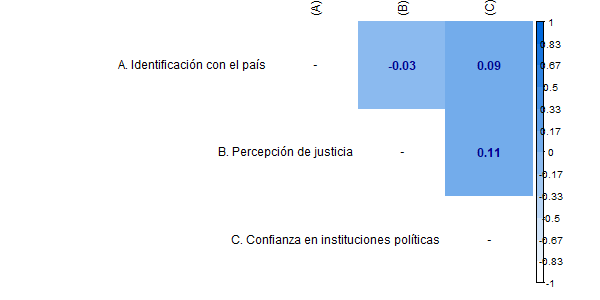
\includegraphics[width=1\linewidth,height=1\textheight]{output/graphs/pertenencia_cor} 

}

\caption{Asociación de las subdimensiones de Sentido de pertenencia}\label{fig:sentido-pertenencia}
\end{figure}

\hypertarget{orientaciuxf3n-hacia-el-bien-comuxfan}{%
\section{Orientación hacia el bien común}\label{orientaciuxf3n-hacia-el-bien-comuxfan}}

Esta tercera dimensión refiere a ``una actitud favorable a acciones que propendan a un mayor bienestar colectivo versus el beneficio puramente individual como parte de un proyecto compartido, o bien, como indican Sorj y Tironi (2007), aceptar ``vivir en un orden colectivo que les reportará beneficios, así como sacrificios individuales''.'' (\protect\hyperlink{ref-cepal_cohesion_2021}{CEPAL, 2021, p. 46})

\textbf{Solidaridad}

La subdimensión de solidaridad busca cuantificar la presencia de valores solidarios en los individuos de la sociedad. Esta solidaridad se basa en el ``entendimiento de la reciprocidad aprendida en redes, y es un reflejo de la solidaridad que perciben recibir por parte del Estado y sus pares (CEPAL, 2007)'' (\protect\hyperlink{ref-cepal_cohesion_2021}{CEPAL, 2021, p. 66}).

En informe CEPAL utilizan el indicador ``Asistencia a reuniones de un grupo de mejoras para la comunidad'', que cuantifica la asistencia a reuniones para mejorar su comunidad. Al trabajar con ELSOC se utilizará este item y otros siete que abordan un comportamiento prosocial y que están presentes en las cinco olas. Un análisis descriptivo de estos items se presentan en la Figura \ref{fig:solidaridad} y un análisis bivariado en la Figura \ref{fig:solidaridad-cor}. Para estos análisis se consideraron solo a las personas que participaron en las cinco olas, pero con sus respuestas de la ola 1 (2016). La tasa de respuesta considera un n de alrededor de 1880 respuestas.

\begin{figure}[H]

{\centering 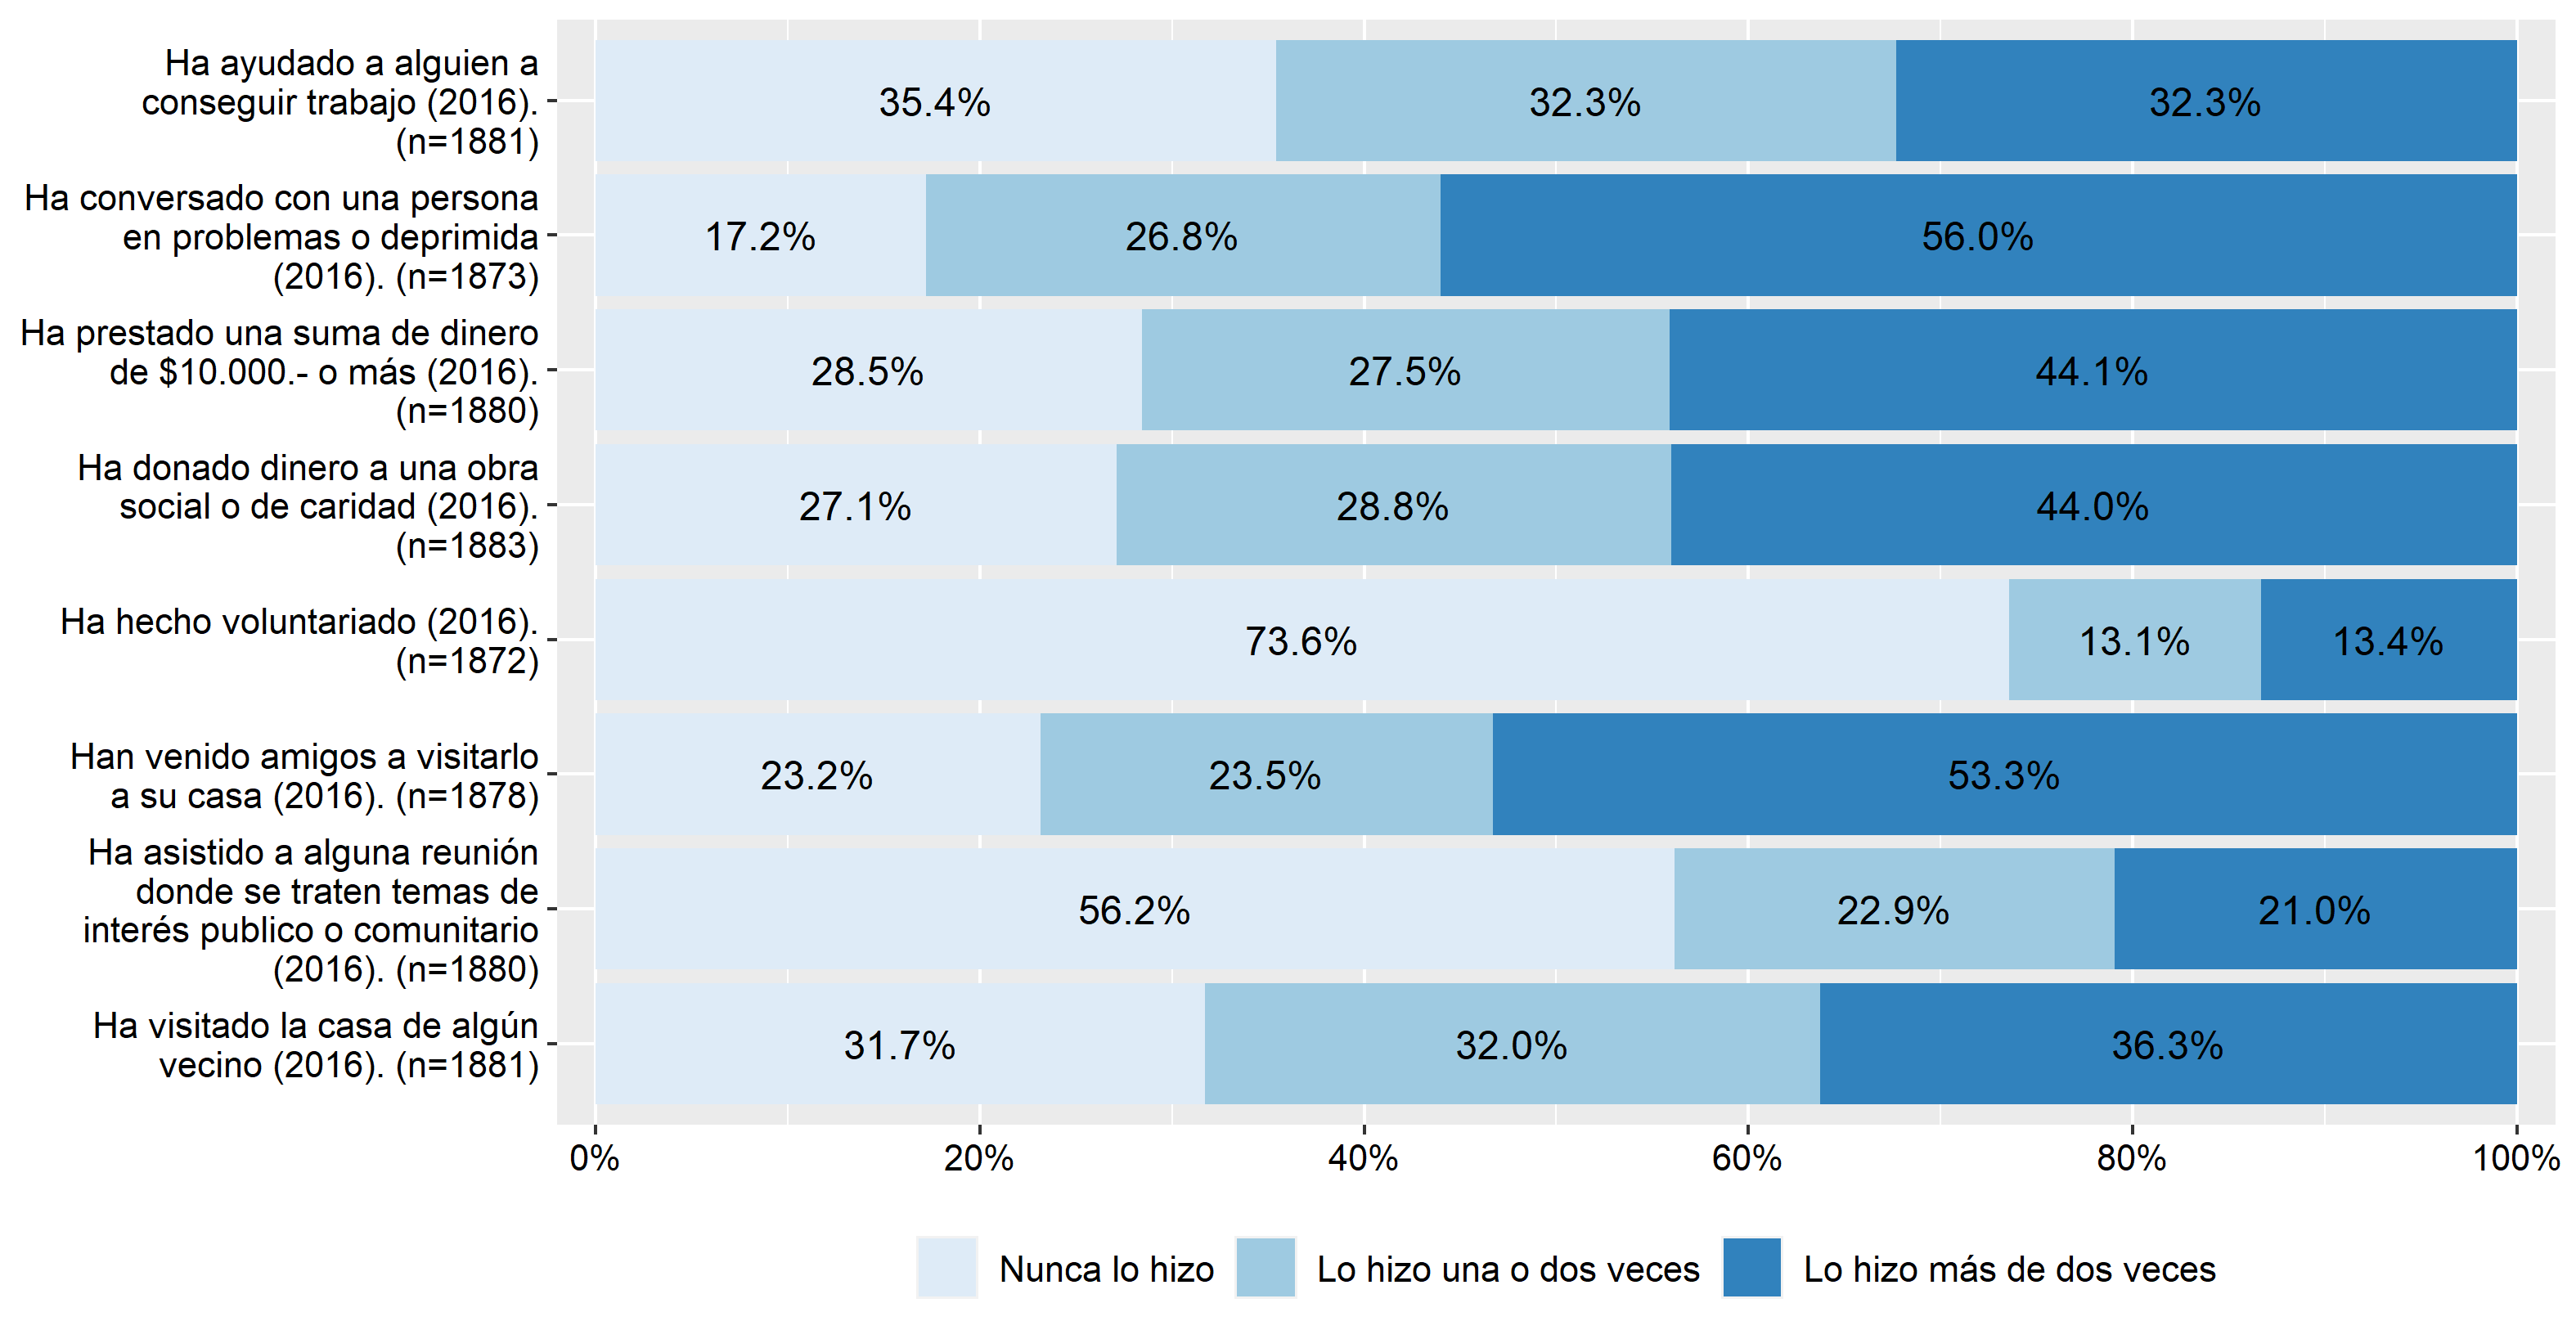
\includegraphics[width=1\linewidth,height=1\textheight]{output/graphs/solidaridad} 

}

\caption{Acciones de solidaridad.}\label{fig:solidaridad}
\end{figure}

\begin{figure}[H]

{\centering 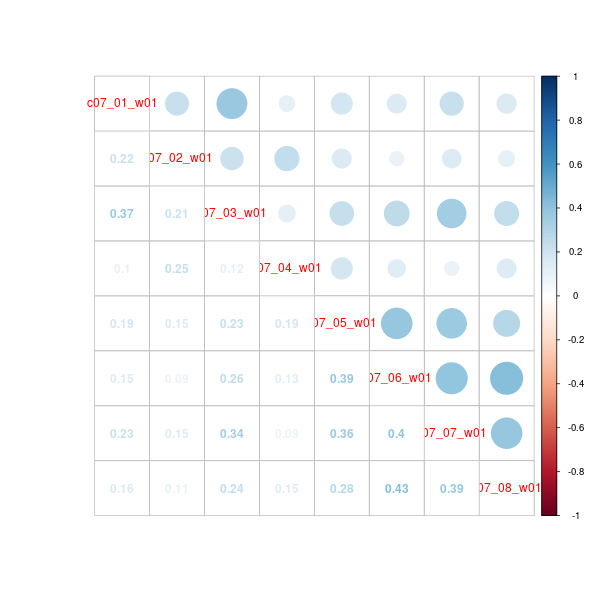
\includegraphics[width=1\linewidth,height=1\textheight]{output/graphs/solidaridad_cor} 

}

\caption{Asociación indicadores de solidaridad.}\label{fig:solidaridad-cor}
\end{figure}

Como esta subdimensión posee ocho items, se volvió a realizar un análisis factorial exploratorio para construir un índice a partir de la información de las dimensiones comunes entre este conjunto de items. La Tabla \ref{tab:solidaridad-fa} nos muestra el resultado de la extracción de tres factores:

\begin{longtable}[]{@{}l@{}}
\caption{\label{tab:solidaridad-fa}Dimensiones de solidaridad.}\tabularnewline
\toprule
\endhead

\includegraphics[width=8.33333in,height=\textheight]{output/tables/solidaridad_fa.png} \\
\bottomrule
\end{longtable}

En la Tabla \ref{tab:inst-fa} es posible observar en la segunda columna (ML1) un factor relacionado con acciones de solidaridad como prestar o donar dinero, ayudar a una persona a conseguir trabajo y conversar con una persona con problemas o deprimida, luego en la tercera columna (ML3) se presenta un segundo factor asociado con la participación en reuniones sociales, como visitar casas de vecinos, recibir visitas de amigos o asistir a reuniones donde se traten problemas relevantes para la comunidad. Finalmente, en la cuarta columna (ML2) se observa un tercer factor que posee un item sobre realizar trabajo voluntario. En relación con la varianza que se asocia a cada uno de estos factores, el primer factor representa un 19\% de la varianza, el segundo un 12\% y el tercero un 9\%. Por lo tanto, se propone utilizar un índice asociado al primer factor que incluye los items ``Ha prestado una suma de dinero de \$10.000.- o más'', ``Ha ayudado a alguien a conseguir trabajo'', ``Ha conversado con una persona en problemas o deprimida'' y ``Ha donado dinero a una obra social o de caridad''.

\textbf{Participación cívica}

La subdimensión de participación cívica da cuenta de la voluntad de adherir a los espacios de participación del sistema político y la vinculación de los individuos con su comunidad. Esta participación ``promueve la participación ciudadana en los asuntos públcios, apoyando pryectos colectivas que representen sus opiniones o intereses políticos (Valdéz, Viramontes y Finol, 2016)'' (\protect\hyperlink{ref-cepal_cohesion_2021}{CEPAL, 2021, p. 66}).

En informe CEPAL se utilizaron los indicadores ``Tiene actividad política (firma peticiones, boicot, va a manifestaciones pacíficas, huelgas)'', que indica la predisposición hacia la actividad política, ``Participación en organizaciones'', que busca medir la implicación de los individuos con su comunidad y ``Voto en elecciones presidenciales'', que pretende capturar el grado de compromiso cívico con el sistema regente y la dirección de la sociedad. Al trabajar con ELSOC se utilizan cuatro items de actividad política presentes en las cuatro primeras olas, ocho items de participación en organizaciones presentes en ola 1 y 3 y voto en elecciones 2013 y 2017 (ola 1 y 3). Un análisis descriptivo de estos items se presentan en la Figura \ref{fig:participacion-civica}, en la Figura \ref{fig:participacion-organizaciones} y en la Figura \ref{fig:participacion-electoral}, mientras que un análisis bivariado en la Figura \ref{fig:participacion-civica-cor} y en la Figura \ref{fig:participacion-organizaciones-cor}. Para estos análisis se consideraron solo a las personas que participaron en las olas mencionadas, pero se utilizan sus respuestas de la ola 1 (2016). La tasa de respuesta considera un n de alrededor de 1880 respuestas.

\begin{figure}[H]

{\centering 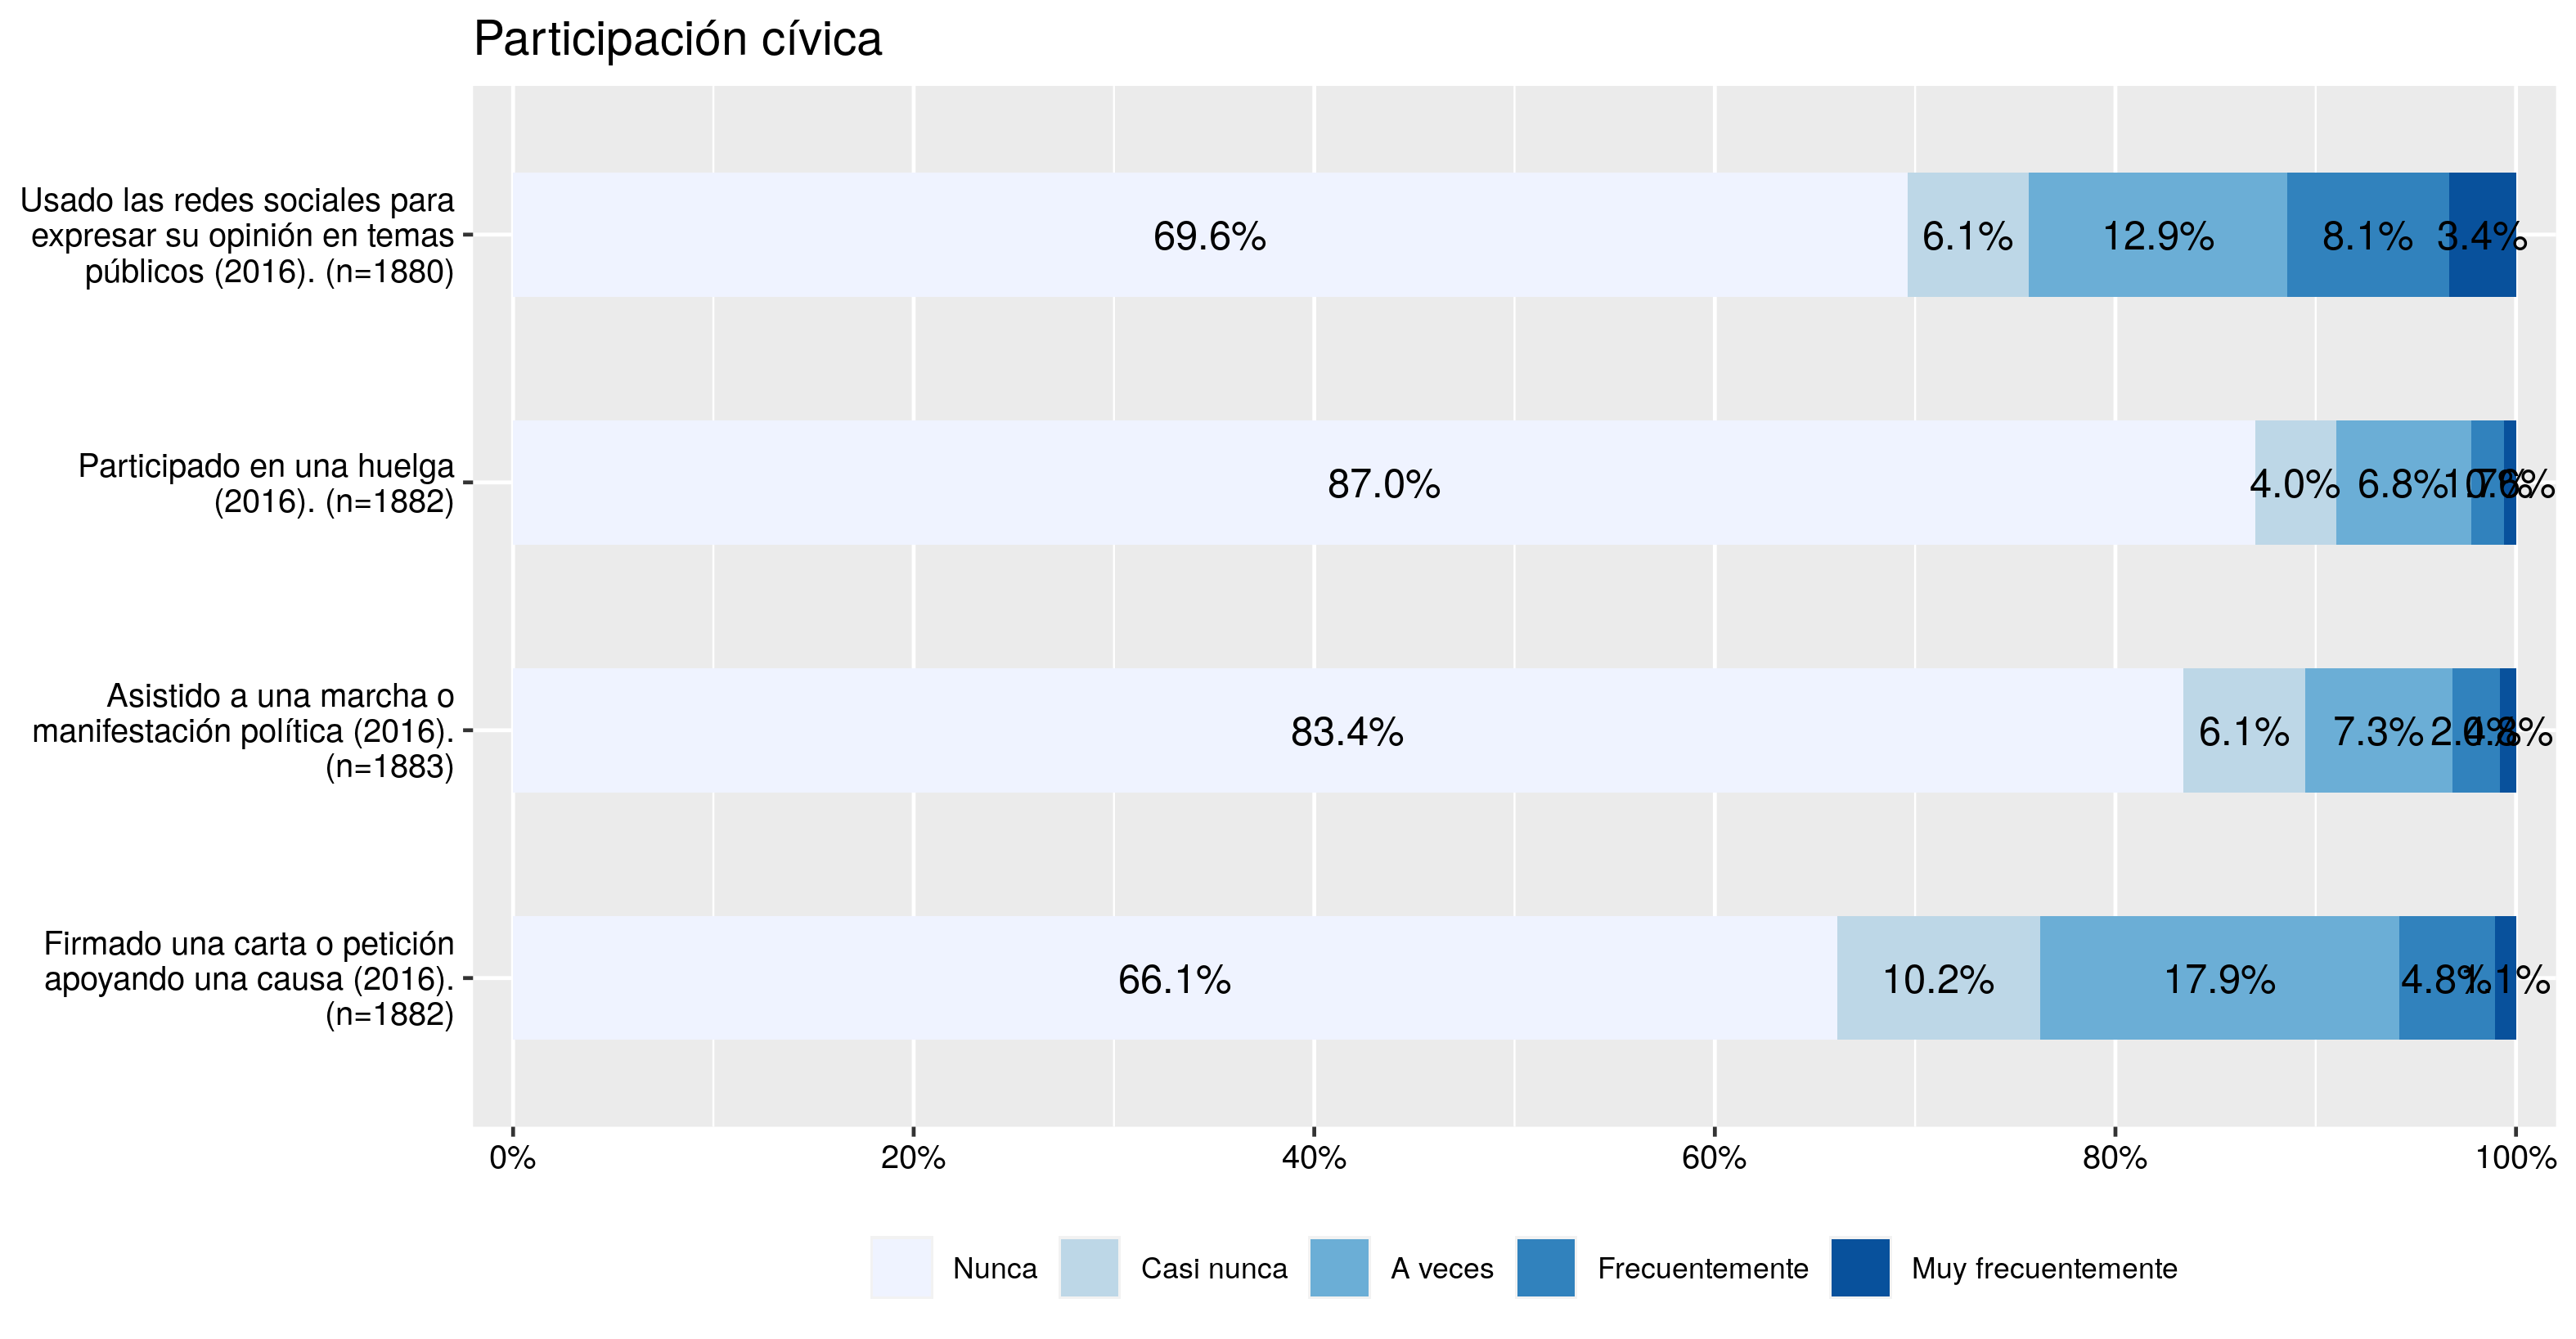
\includegraphics[width=1\linewidth,height=1\textheight]{output/graphs/participacion-civica} 

}

\caption{Participación en actividades cívicas.}\label{fig:participacion-civica}
\end{figure}

\begin{figure}[H]

{\centering 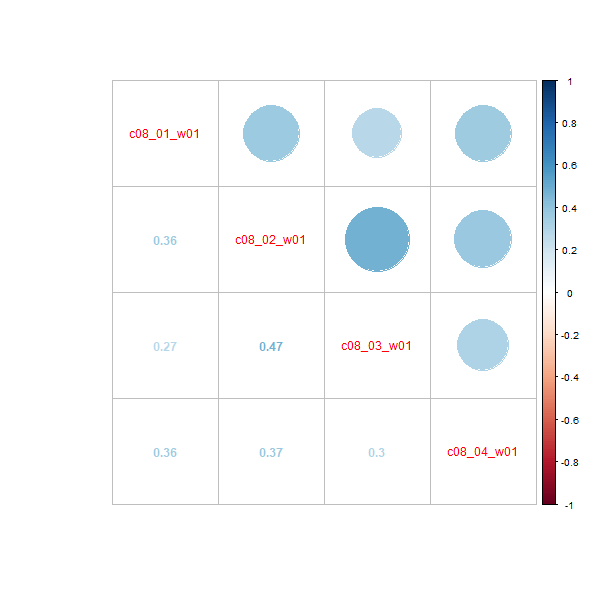
\includegraphics[width=1\linewidth,height=1\textheight]{output/graphs/participacion-civica_cor} 

}

\caption{Asociación indicadores participación cívica.}\label{fig:participacion-civica-cor}
\end{figure}

\textbf{Participación en organizaciones}

\begin{figure}[H]

{\centering 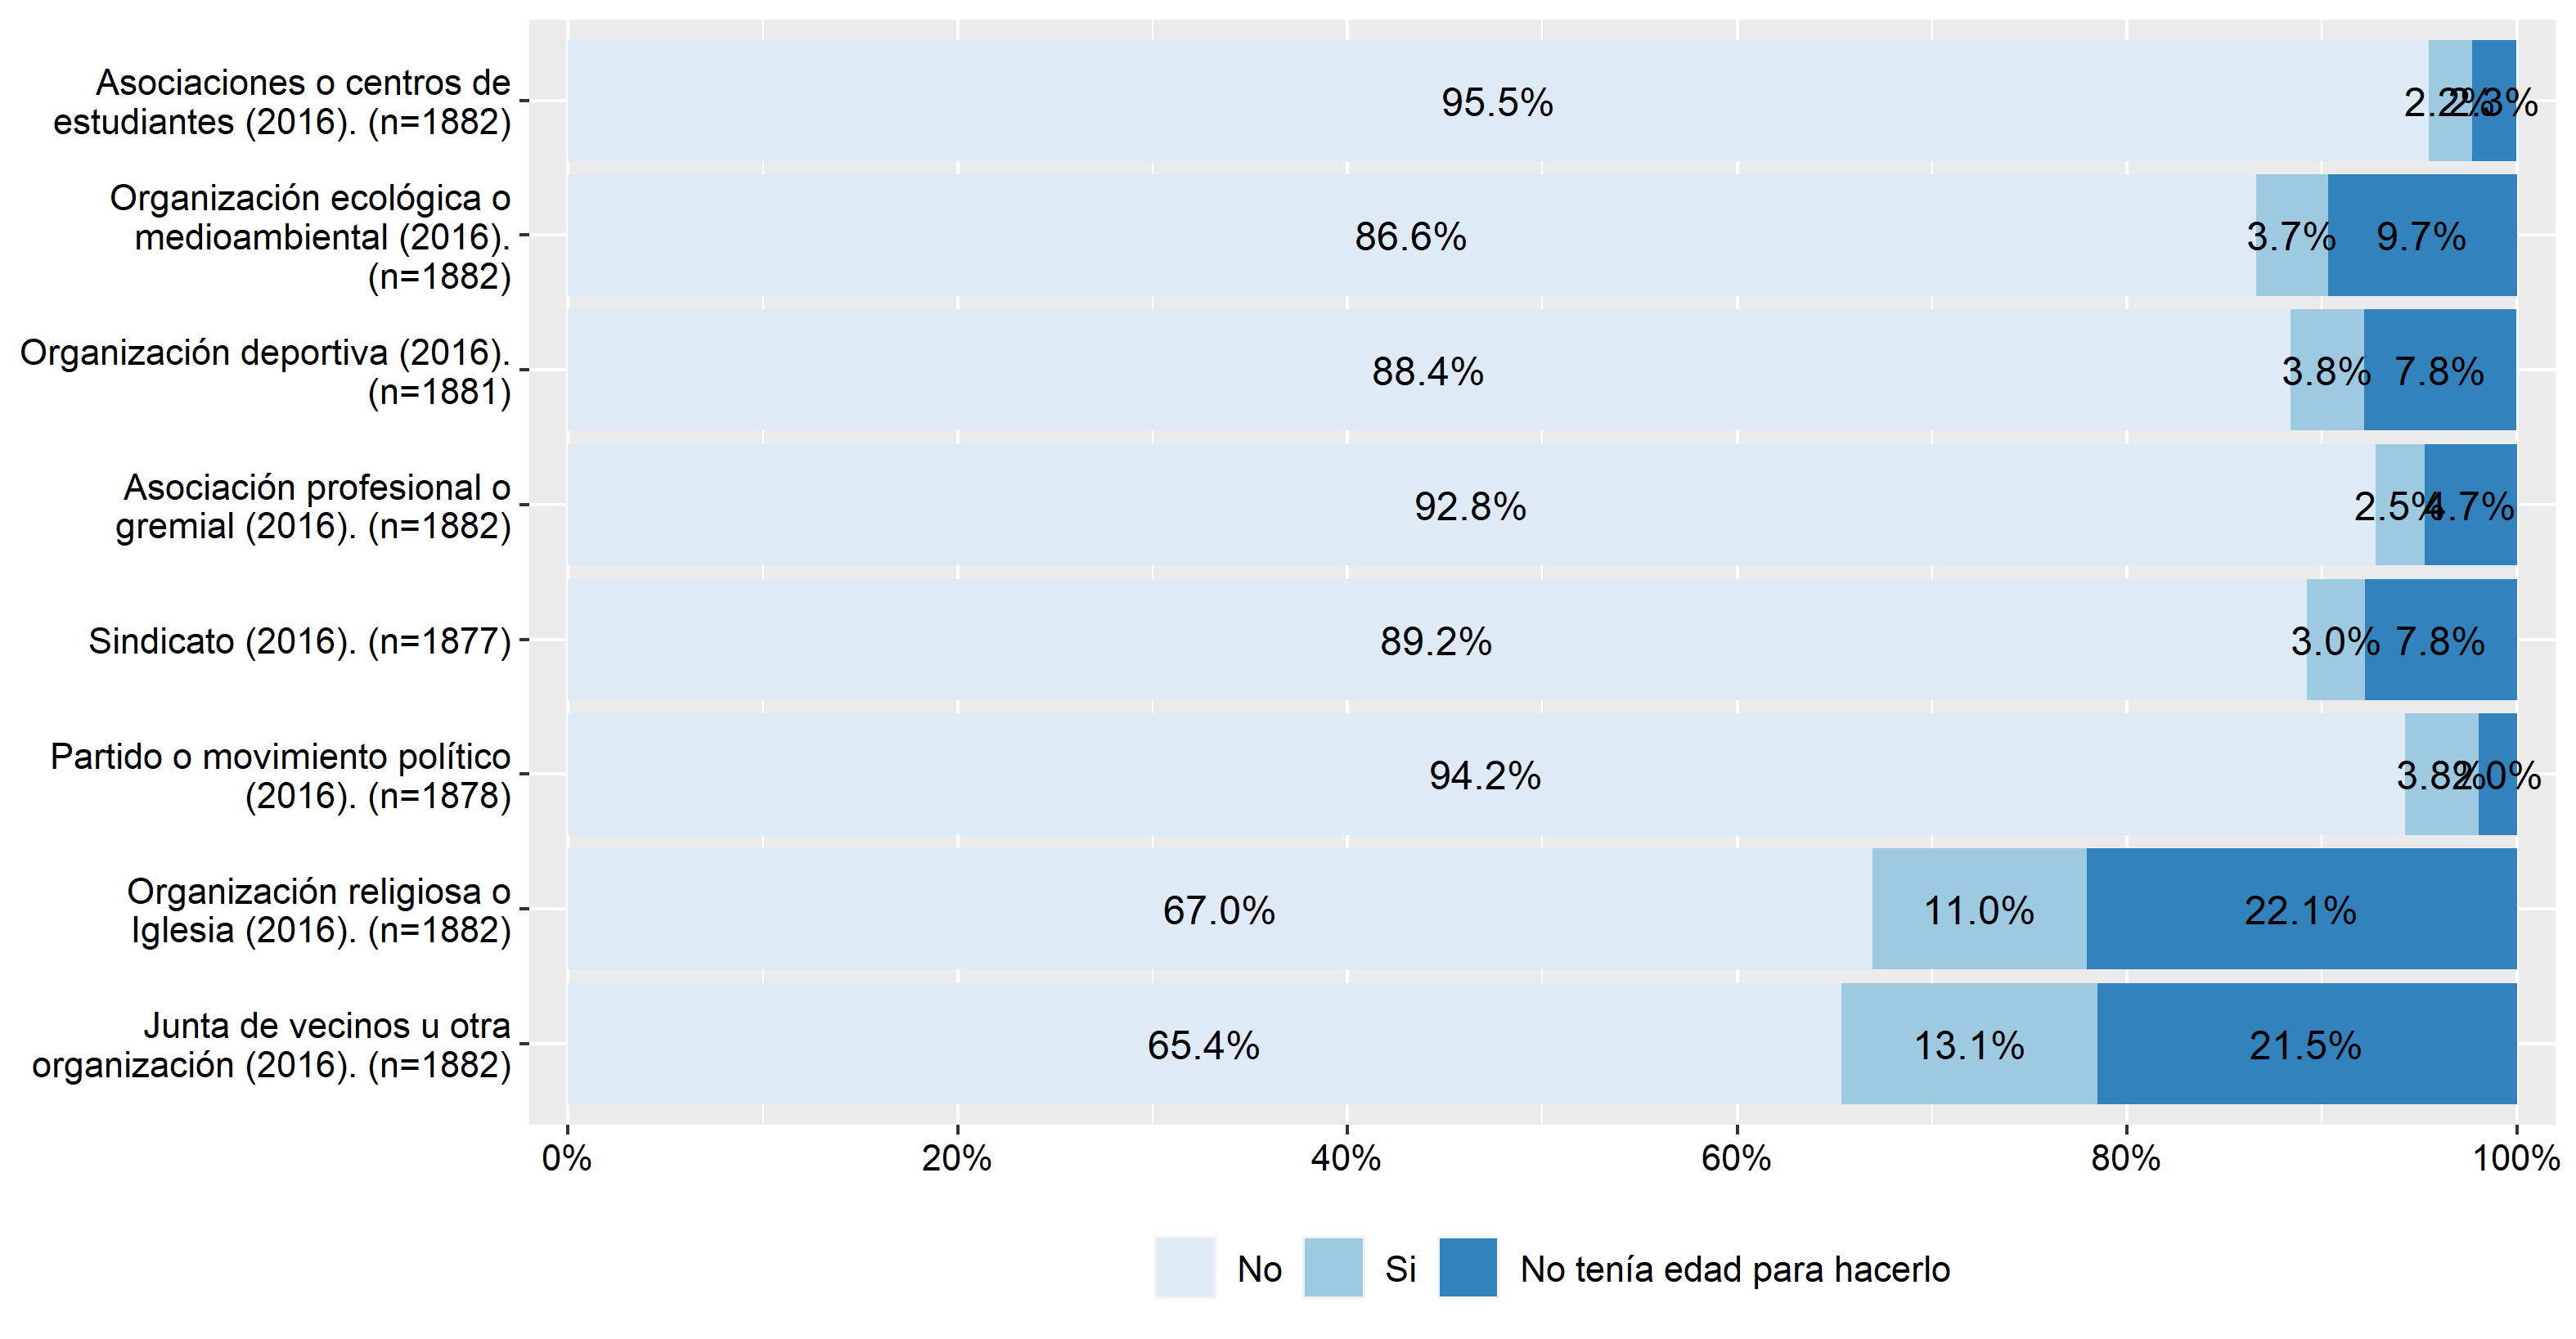
\includegraphics[width=1\linewidth,height=1\textheight]{output/graphs/participacion-organizaciones} 

}

\caption{Participación en organizaciones sociales.}\label{fig:participacion-organizaciones}
\end{figure}

\begin{figure}[H]

{\centering 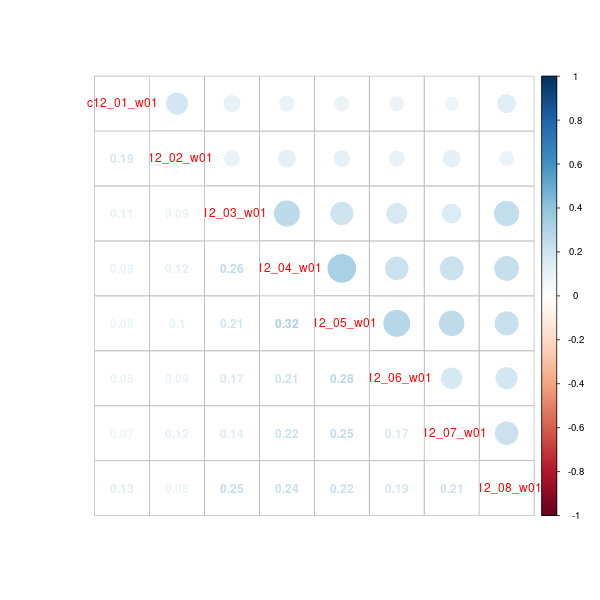
\includegraphics[width=1\linewidth,height=1\textheight]{output/graphs/participacion-organizaciones_cor} 

}

\caption{Asociación indicadores participación en organizaciones.}\label{fig:participacion-organizaciones-cor}
\end{figure}

\textbf{Participación electoral}

\begin{figure}[H]

{\centering 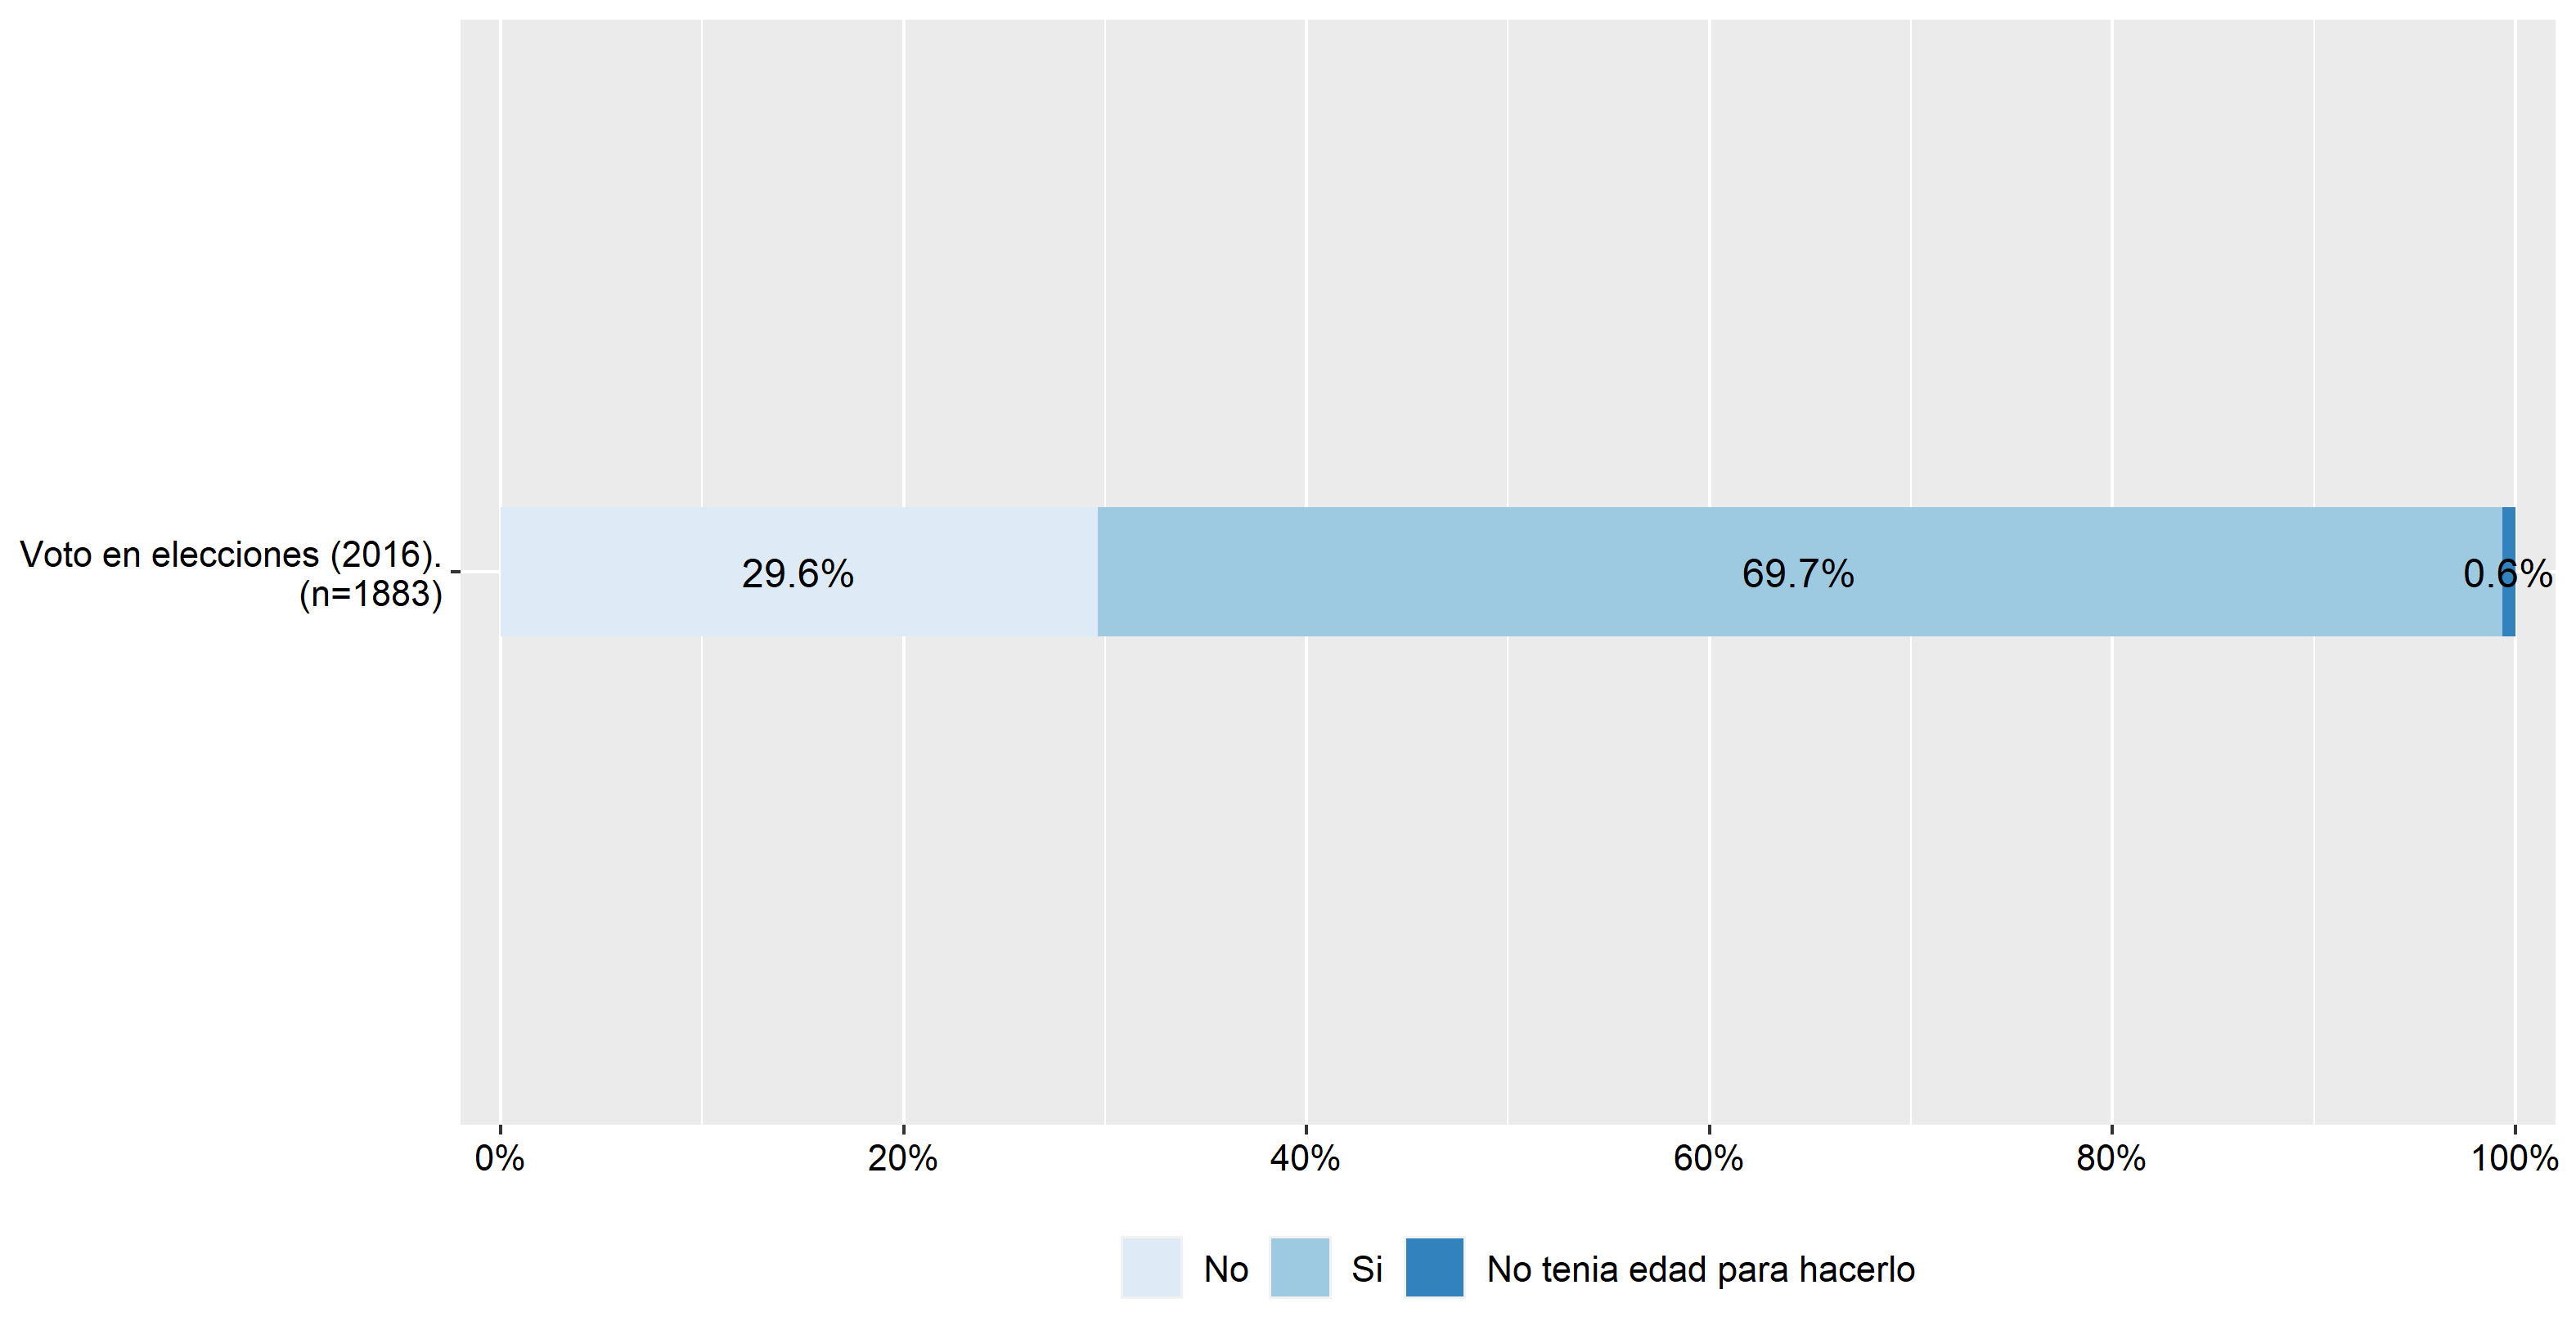
\includegraphics[width=1\linewidth,height=1\textheight]{output/graphs/participacion-electoral} 

}

\caption{Participación en elecciones 2013 y 2017.}\label{fig:participacion-electoral}
\end{figure}

En esta oportunidad, se utilizó un análisis factorial exploratorio sobre los cuatro items de participación cívica, sobre los ocho tipos de participación en organizaciones presentes en ELSOC y sobre el item de participación en elecciones con el objetivo de construir un índice a partir de la información de las dimensiones comunes que subyacen a este conjunto de items. La Tabla \ref{tab:participacion-fa} nos muestra el resultado de la extracción de tres factores:

\begin{longtable}[]{@{}l@{}}
\caption{\label{tab:participacion-fa}Dimensiones de Participación cívica y en organizaciones.}\tabularnewline
\toprule
\endhead

\includegraphics[width=8.33333in,height=\textheight]{output/tables/participacion_fa.png} \\
\bottomrule
\end{longtable}

Podemos observar en la Tabla \ref{tab:participacion-fa} un primer factor asociado a la participación cívica (asitir a marchas, participar en huelgas, expresar opiniones por redes sociales y firmar una carta o petición). Luego se observa un segundo factor que incluye la participación en cinco organizaciones (asociación profesional, organización deportiva, sindicato, centro de estudiantes y partidos políticos). Finalmente, se observa un tercer factor que incluye la participación en una organización religiosa y en juntas de vecinos. En cuanto a la varianza asociada a cada uno de estos factores, el primer factor es el más alto, que representa un 12,5\% de la varianza. El segundo y tercer factor representan un 8\% y 5.5\% respectivamente. Por lo tanto, no existe un grado de consistencia relevante en el segundo y tercer factor, por lo cual se propone no incluir los items asociados a la participación en organizaciones y trabajar solo con los items referentes a participación cívica.

Finalmente, la subdimensión de Respeto por reglas sociales presente en esta dimensión de la propuesta regional de la CEPAL, que posee un indicador de respeto por las instituciones inexistente en el ELSOC, no será considerada. Así, la correlación entre los dos indicadores propuestos para esta dimensión -solidaridad y participación cívica- poseen una correlación de 0.32.

\hypertarget{cohesiuxf3n-territorial}{%
\section{Cohesión territorial}\label{cohesiuxf3n-territorial}}

De manera adicional, se incorpora una dimensión sobre calidad de vida en el vecindario presente en ELSOC. Todos estos items se encuentran presentes en las cuatro olas.

\textbf{Confianza en vecinos}

En la encuesta ELSOC se incluye un item territorial sobre el grado de confianza en vecinos en las cinco olas. Un análisis descriptivo de este item, que sería el único representante de esta subdimensión, se presenta en la Figura \ref{fig:confianza-vecinos}. Este análisis fue realizado solo con las personas que participaron en las cinco olas, pero se utilizan sus respuestas de la ola 1 (n=1876)

\begin{figure}[H]

{\centering 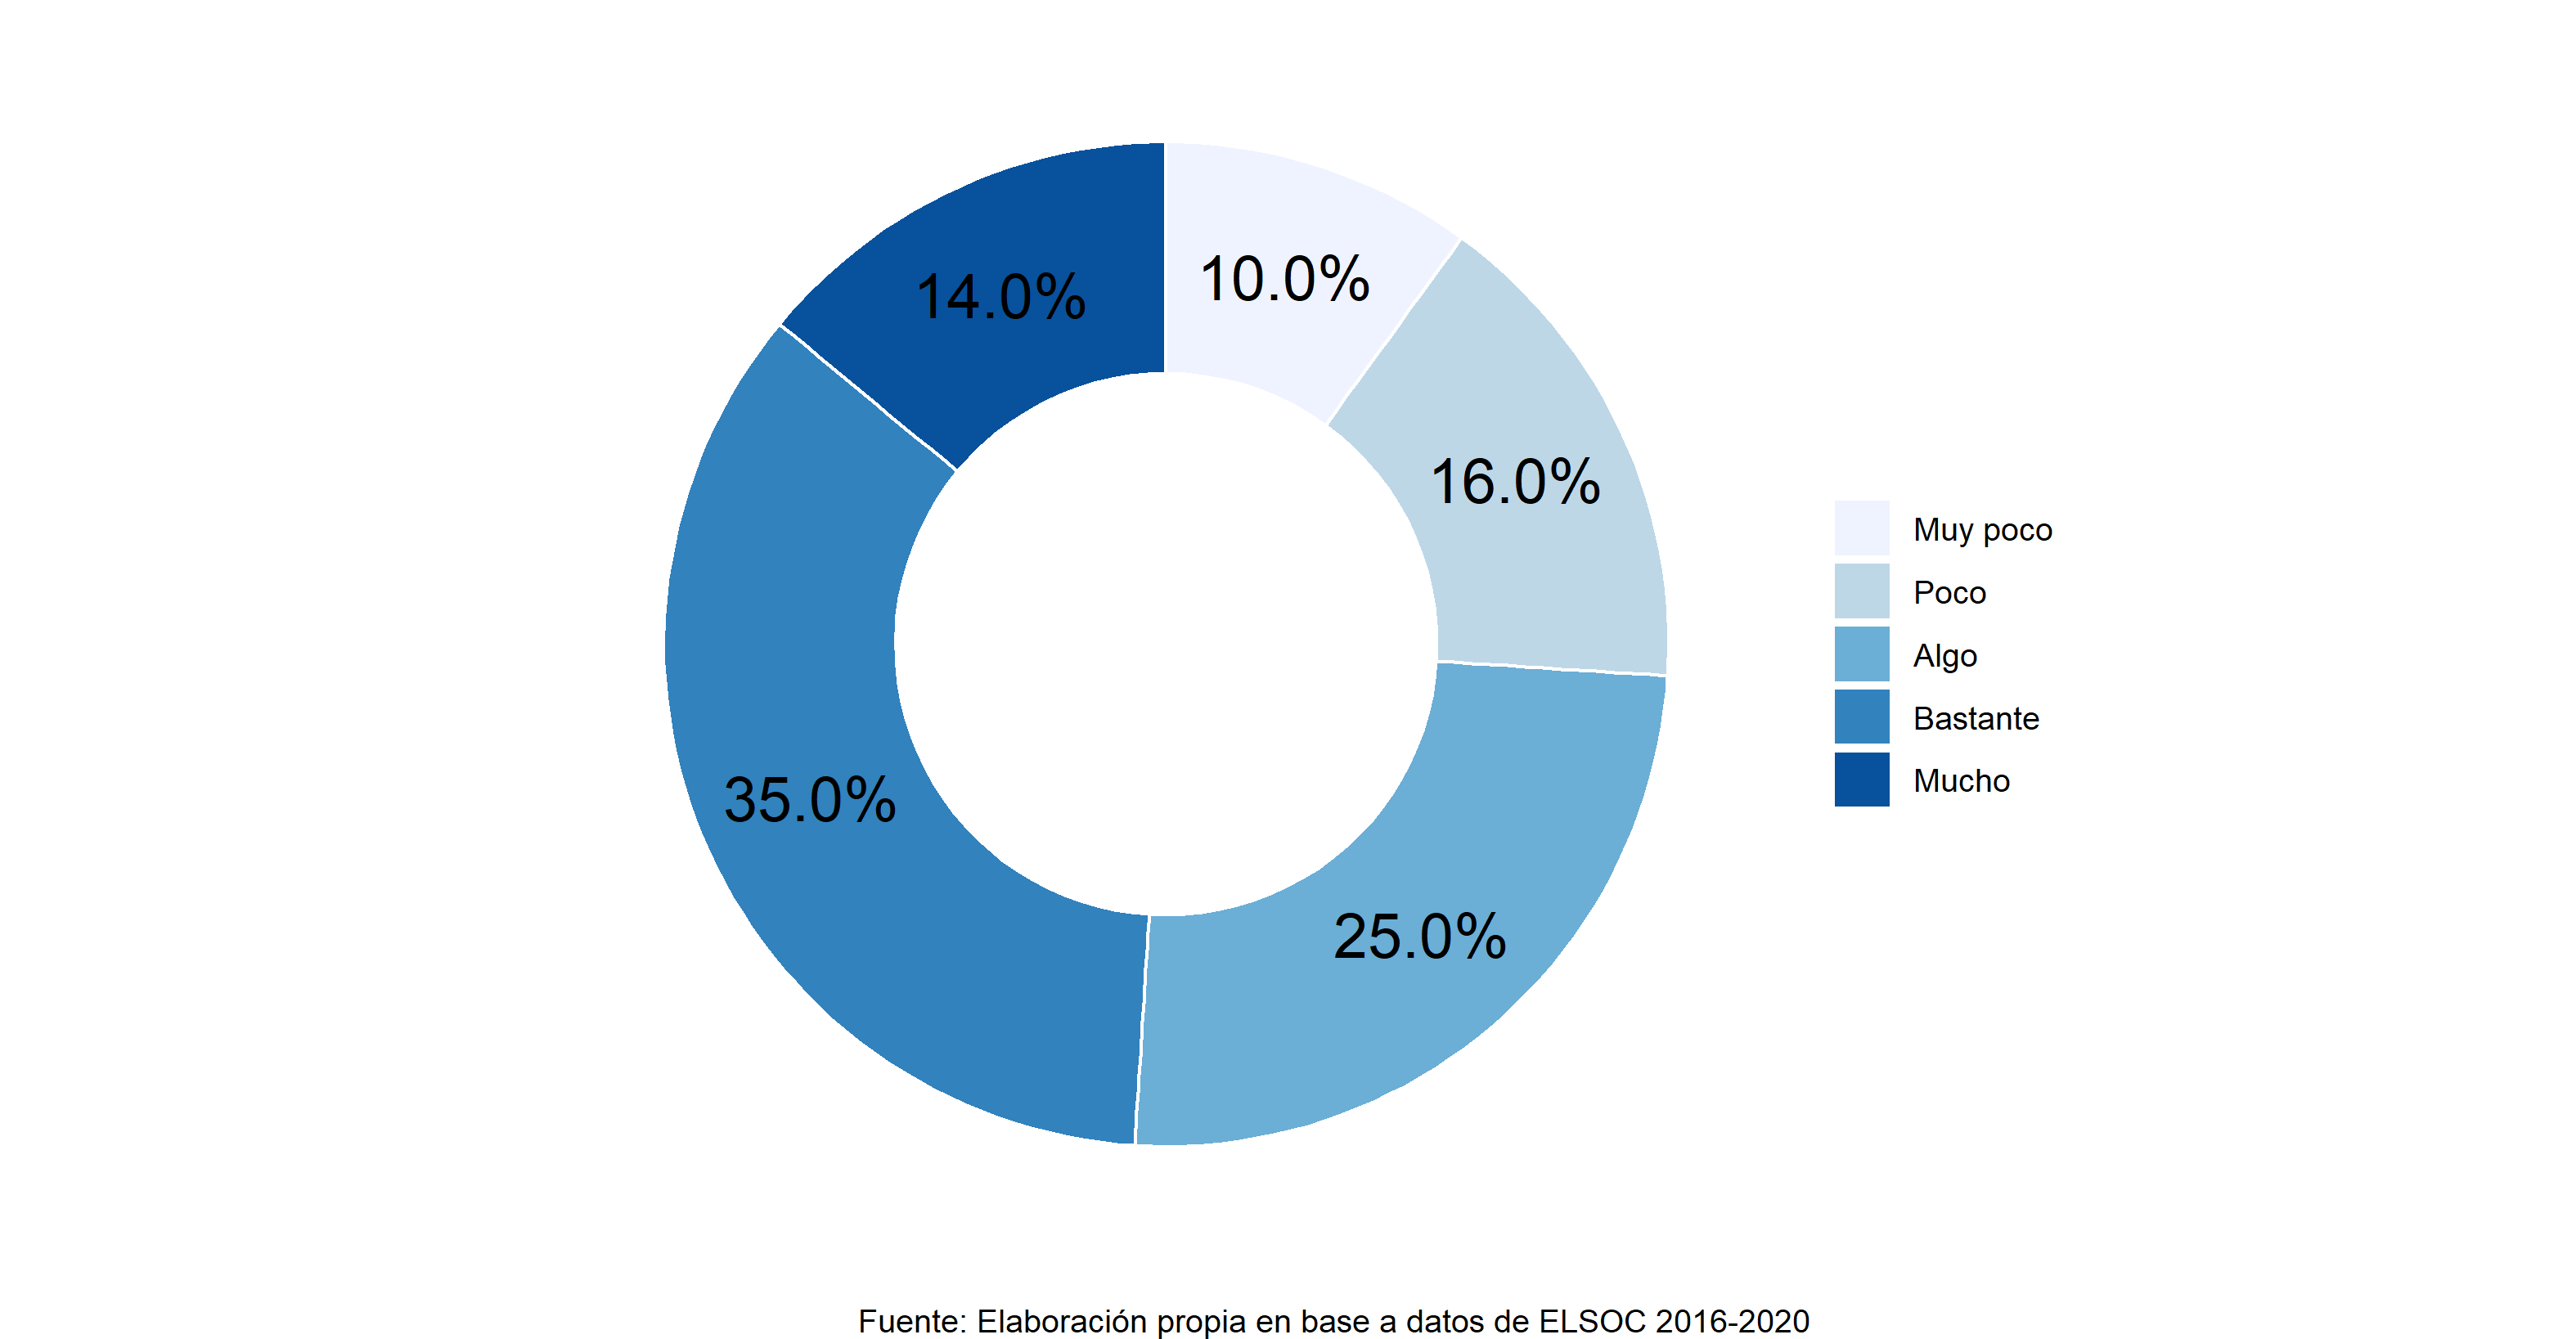
\includegraphics[width=1\linewidth,height=1\textheight]{output/graphs/confianza-vecinos} 

}

\caption{Confianza en vecinos.}\label{fig:confianza-vecinos}
\end{figure}

\textbf{Cohesión barrial}

Otros items territoriales presentes en ELSOC están asociados con la subdimensión de Cohesión barrial. Estos items identifican si las personas se sienten identificadas con la gente del barrio, si se sienten integrados, si se sienten parte del barrio y si creen que es su barrio ideal y están presentes en las cinco olas. Un análisis descriptivo de estos cuatro items se presenta en la Figura \ref{fig:cohesion-barrial} y un análisis bivariado en la Figura \ref{fig:cohesion-barrial-cor}. Ambos análisis fueron realizados considerando solo a las personas que participaron en las olas mencionadas, pero utilizando sus respuestas de la ola 1, alcanzando un n aproximado de 1885.

\begin{figure}[H]

{\centering 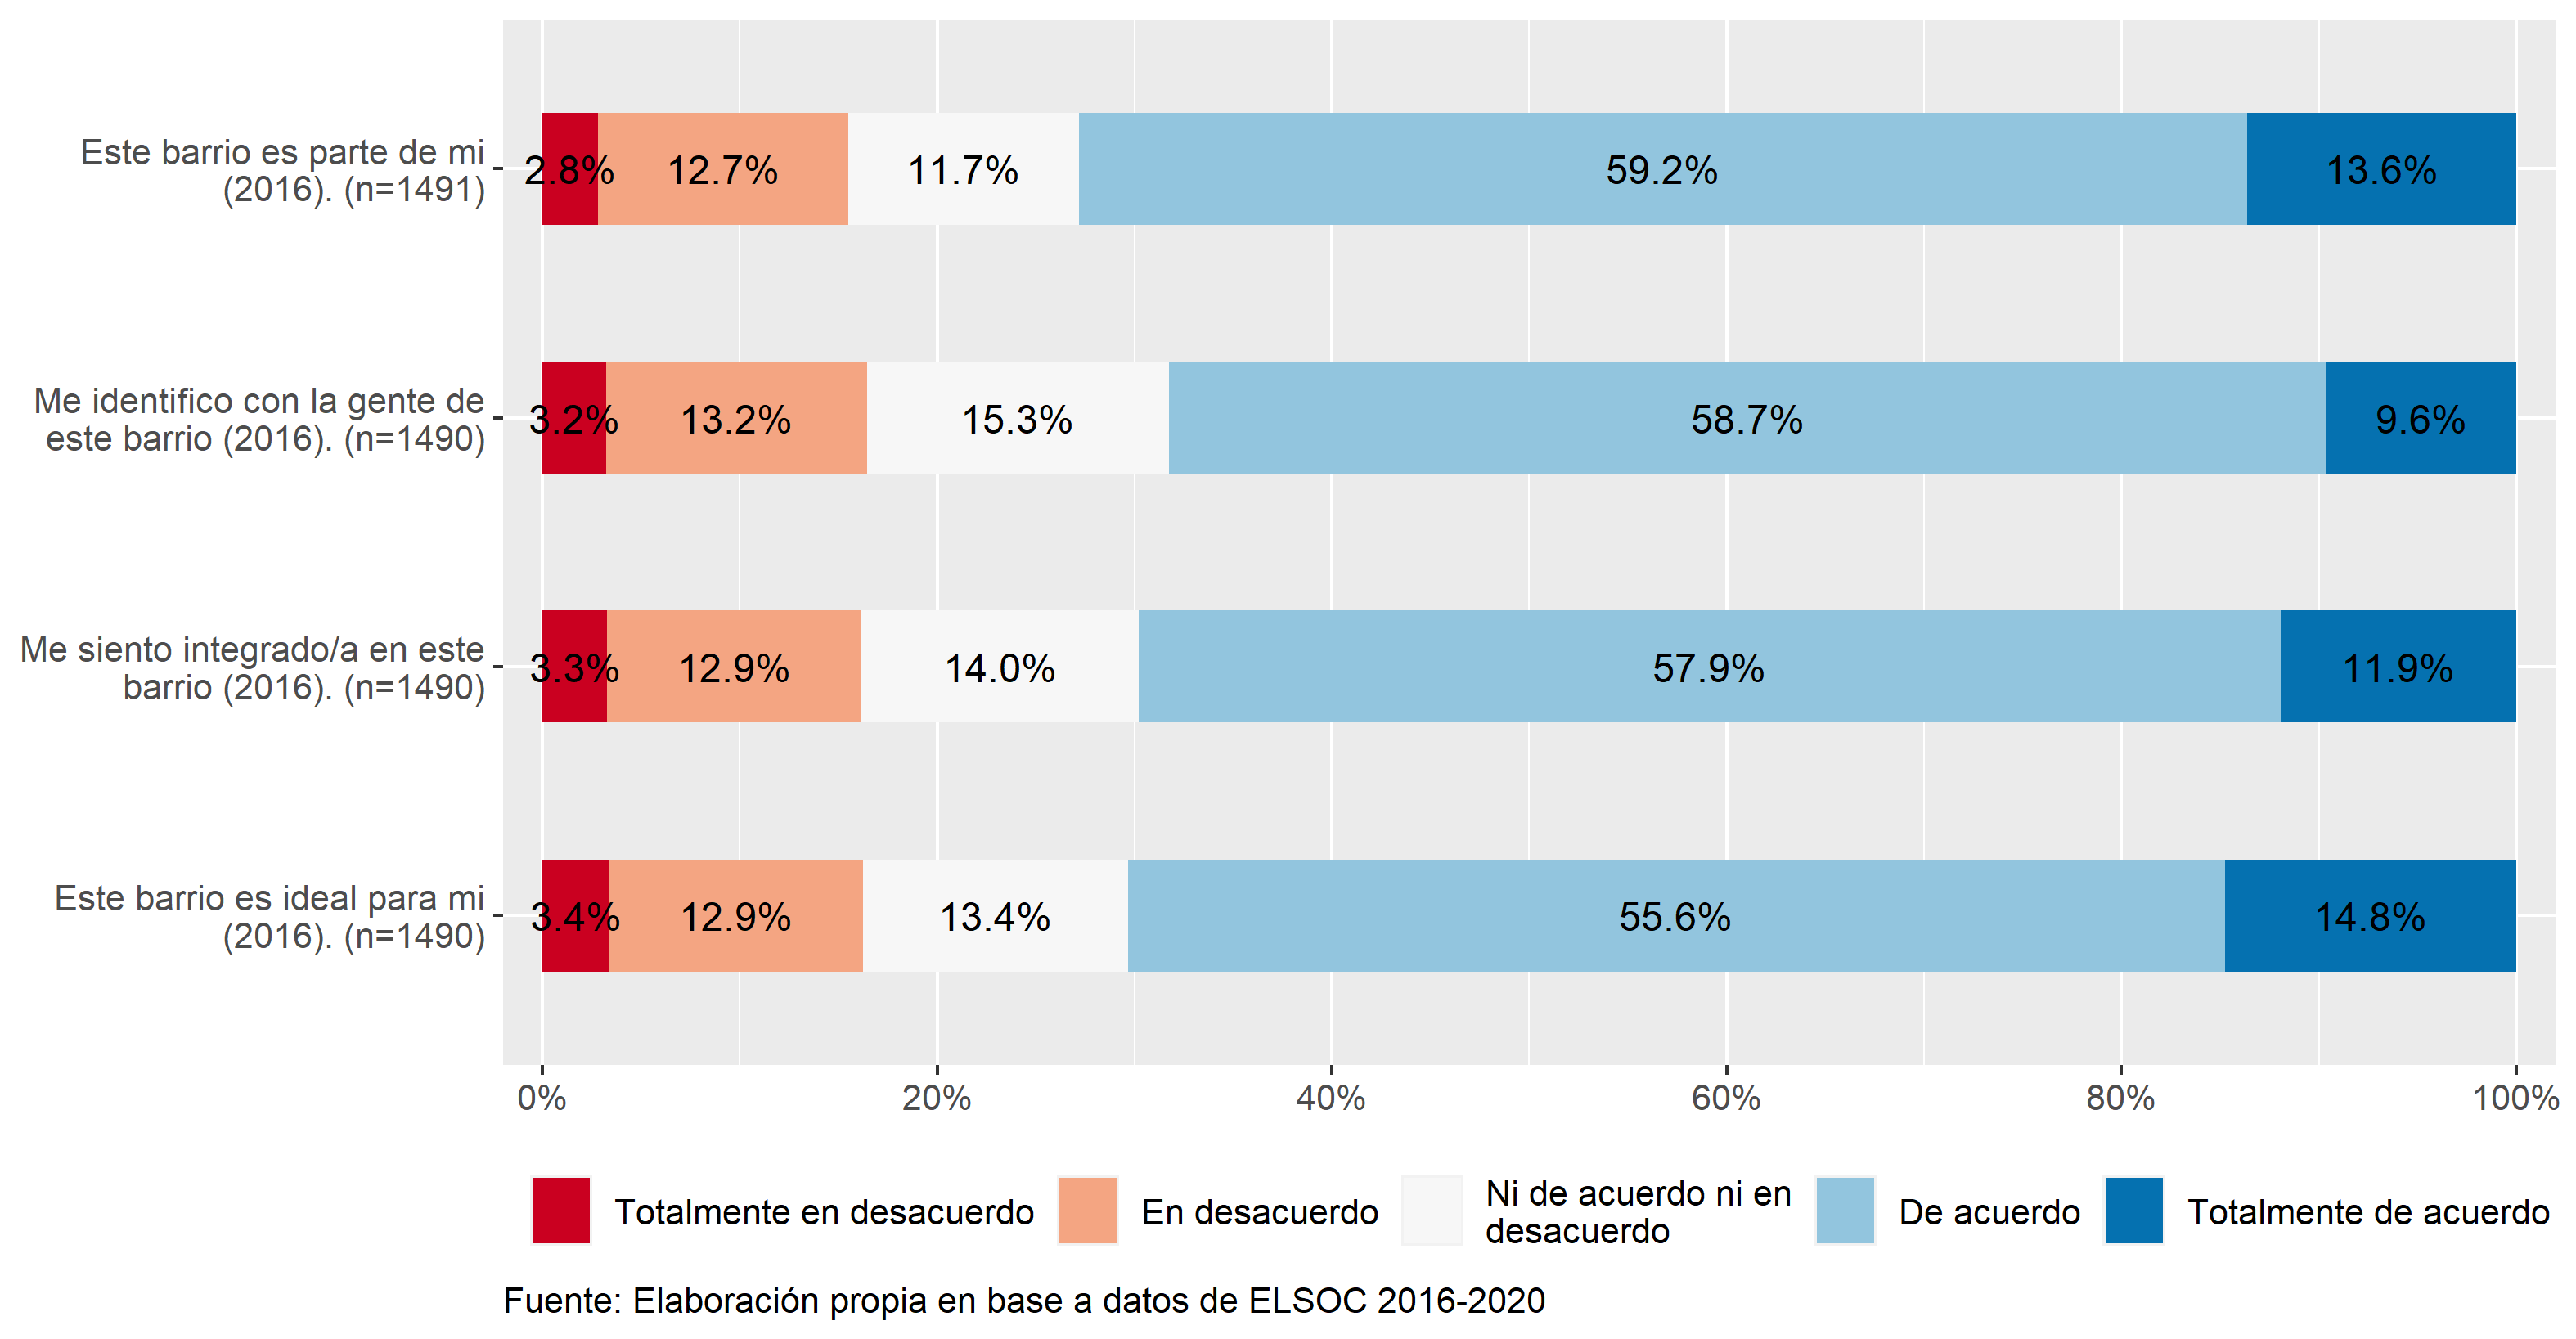
\includegraphics[width=1\linewidth,height=1\textheight]{output/graphs/cohesion-barrial} 

}

\caption{Cohesión en el barrio.}\label{fig:cohesion-barrial}
\end{figure}

\begin{figure}[H]

{\centering 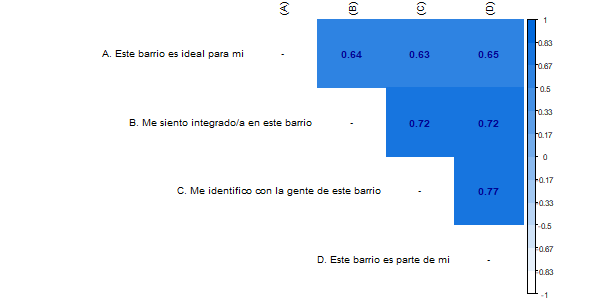
\includegraphics[width=1\linewidth,height=1\textheight]{output/graphs/cohesion-barrial_cor} 

}

\caption{Asociación indicadores cohesión barrial.}\label{fig:cohesion-barrial-cor}
\end{figure}

\textbf{Sociabilidad barrial}

Esta subdimensión de items territoriales aborda la percepción que se tiene sobre el barrio en relación con si las demás personas son sociables, si es fácil hacer amigos, si las personas son cordiales y si son colaboradoras y están presentes en las cinco olas. Un análisis descriptivo de estos cuatro items se presenta en la Figura \ref{fig:sociabilidad-barrial} y un análisis bivariado en la Figura \ref{fig:sociabilidad-barrial-cor}. Ambos análisis fueron realizados considerando solo a las personas que participaron en las olas mencionadas, pero utilizando sus respuestas de la ola 1, alcanzando un n aproximado de 1880.

\begin{figure}[H]

{\centering 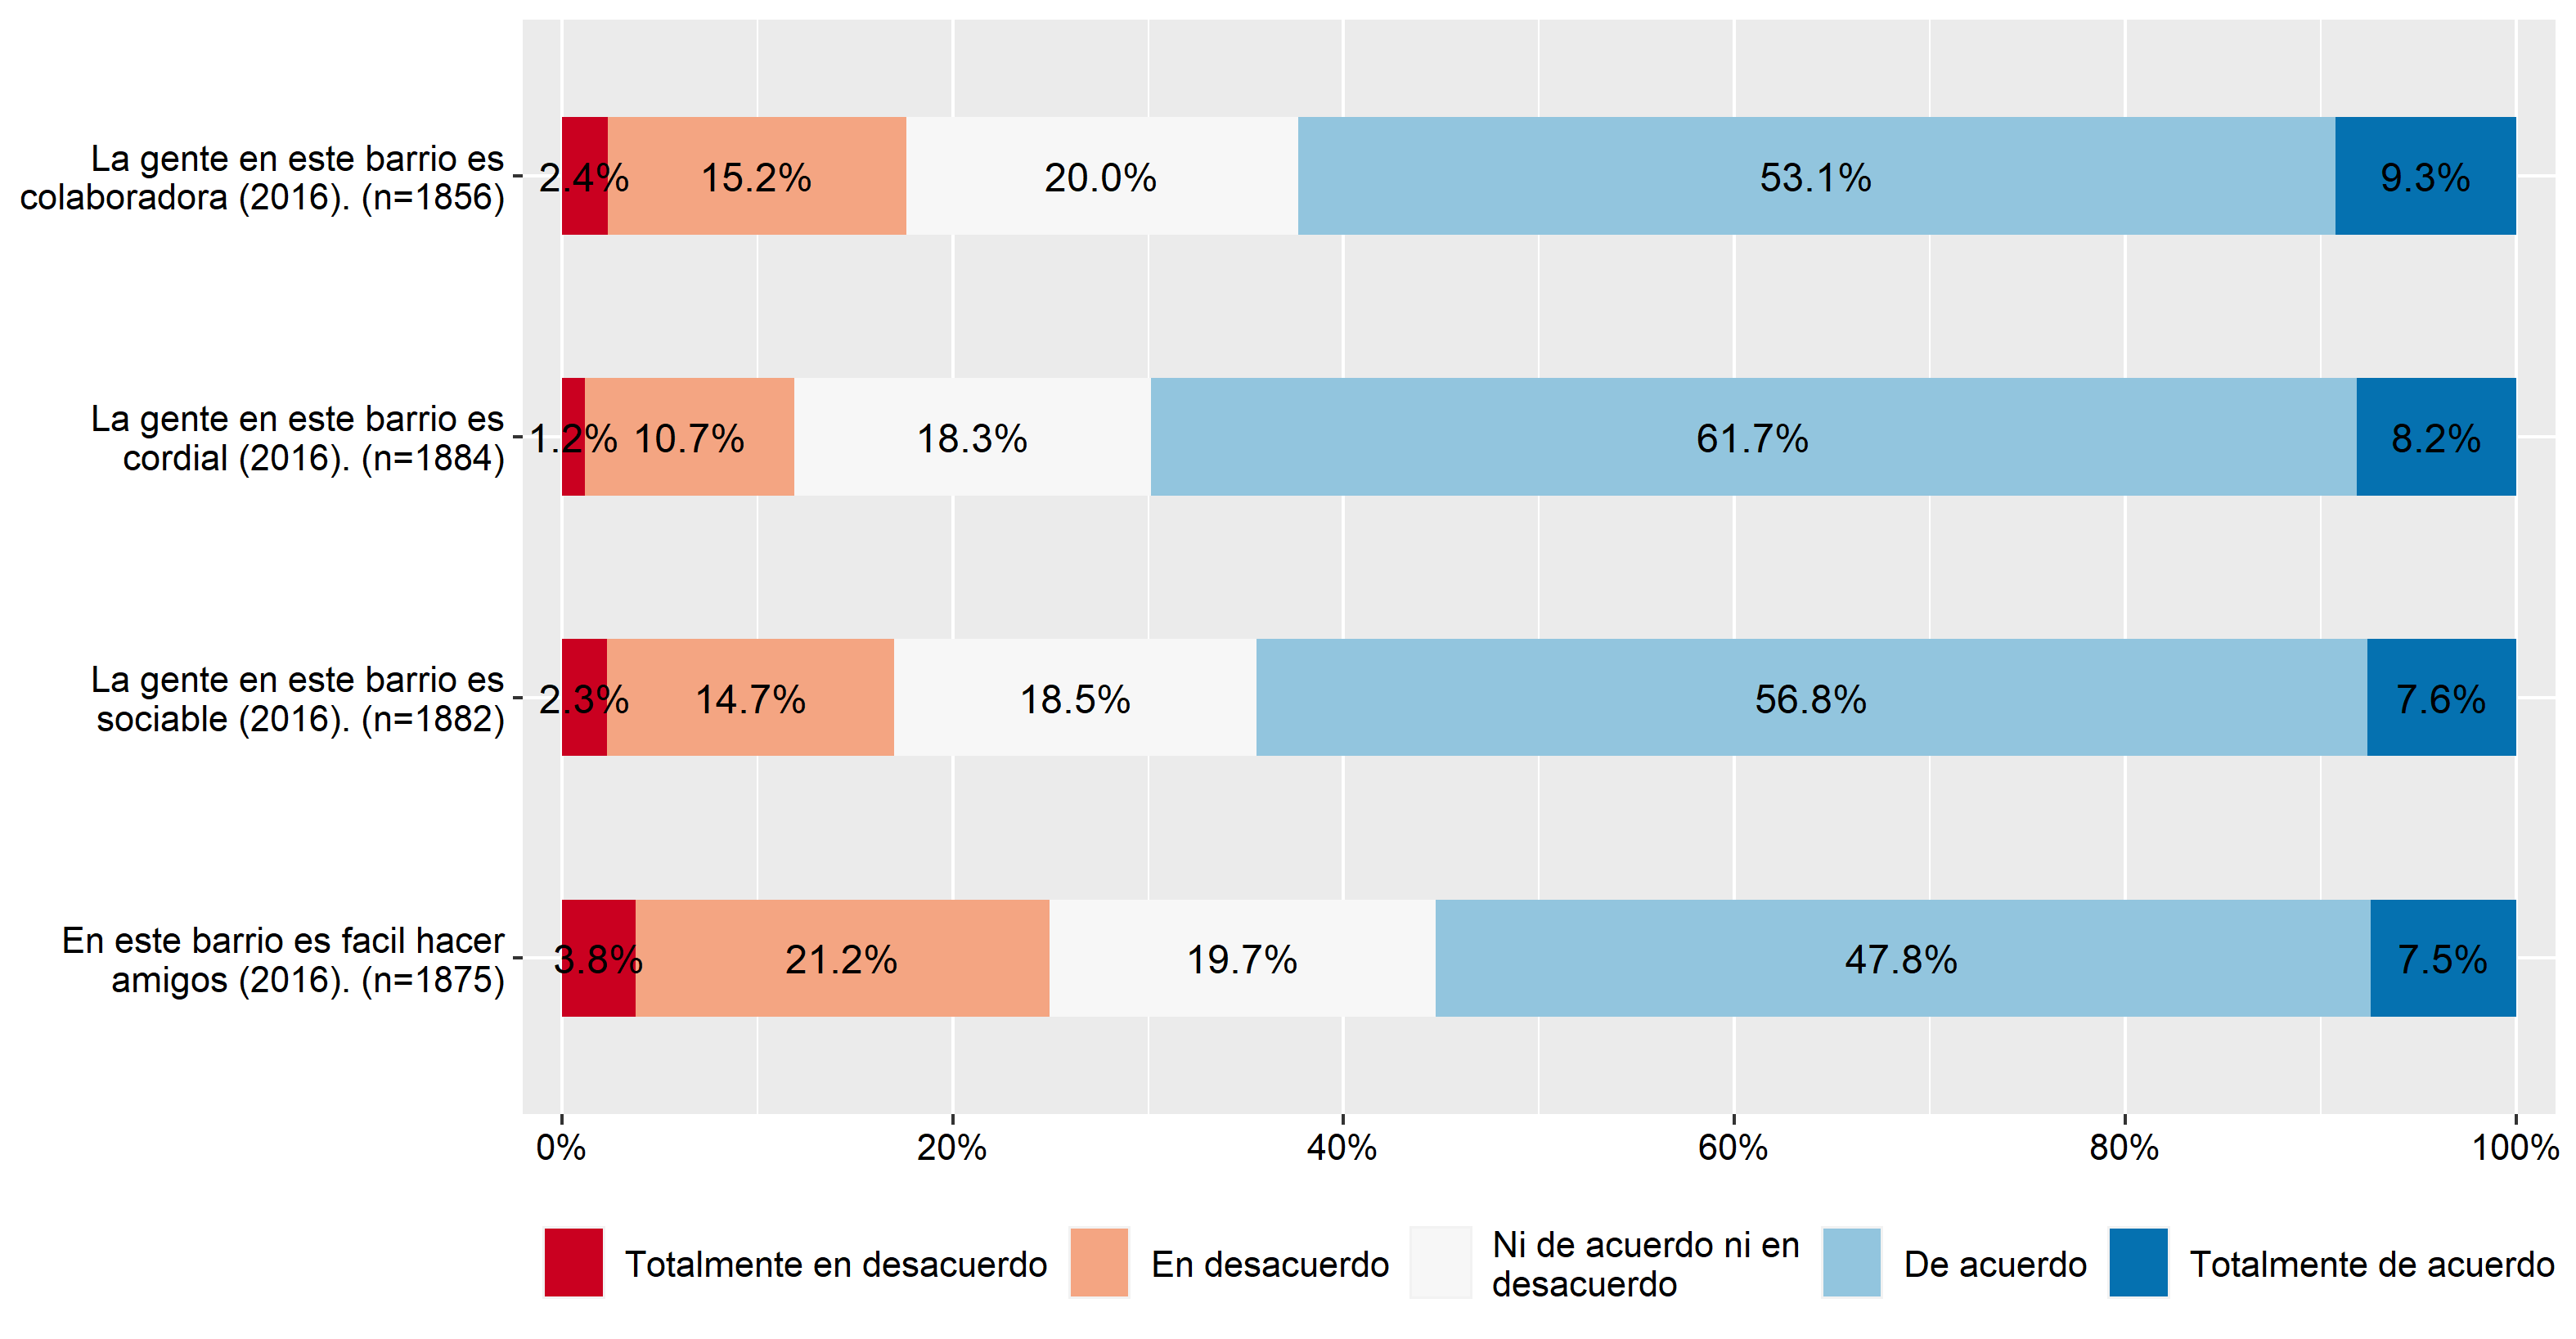
\includegraphics[width=1\linewidth,height=1\textheight]{output/graphs/sociabilidad-barrial} 

}

\caption{Sociabilidad barrial.}\label{fig:sociabilidad-barrial}
\end{figure}

\begin{figure}[H]

{\centering 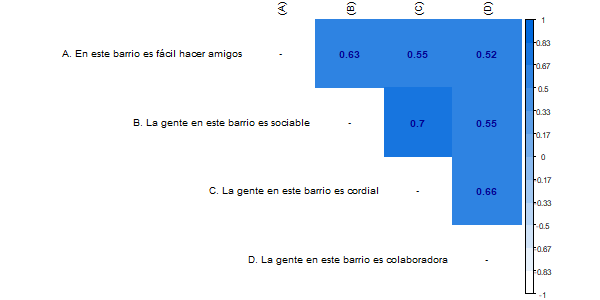
\includegraphics[width=1\linewidth,height=1\textheight]{output/graphs/sociabilidad-barrial_cor} 

}

\caption{Asociación indicadores sociabilidad barrial.}\label{fig:sociabilidad-barrial-cor}
\end{figure}

\textbf{Satisfacción residencial}

Finalmente, se incluye una subdimensión de Satisfacción residencial presente en ELSOC y que está relacionada con items que miden la conectividad del barrio, la proximidad con el comercio, colegios, familiares y la principal actividad de trabajo, la limpieza del barrio, la cantidad de áreas verdes y la seguridad del barrio y están presentes en las cinco olas. Se incluye un análisis descriptivo de estos ocho items en la Figura \ref{fig:satisfaccion-residencial} y un análisis bivariado en la Figura \ref{fig:satisfaccion-residencial-cor}. Ambos análisis fueron realizados considerando solo a las personas que participaron en las olas mencionadas, pero utilizando sus respuestas de la ola 1, alcanzando un n aproximado de 1880.

\begin{figure}[H]

{\centering 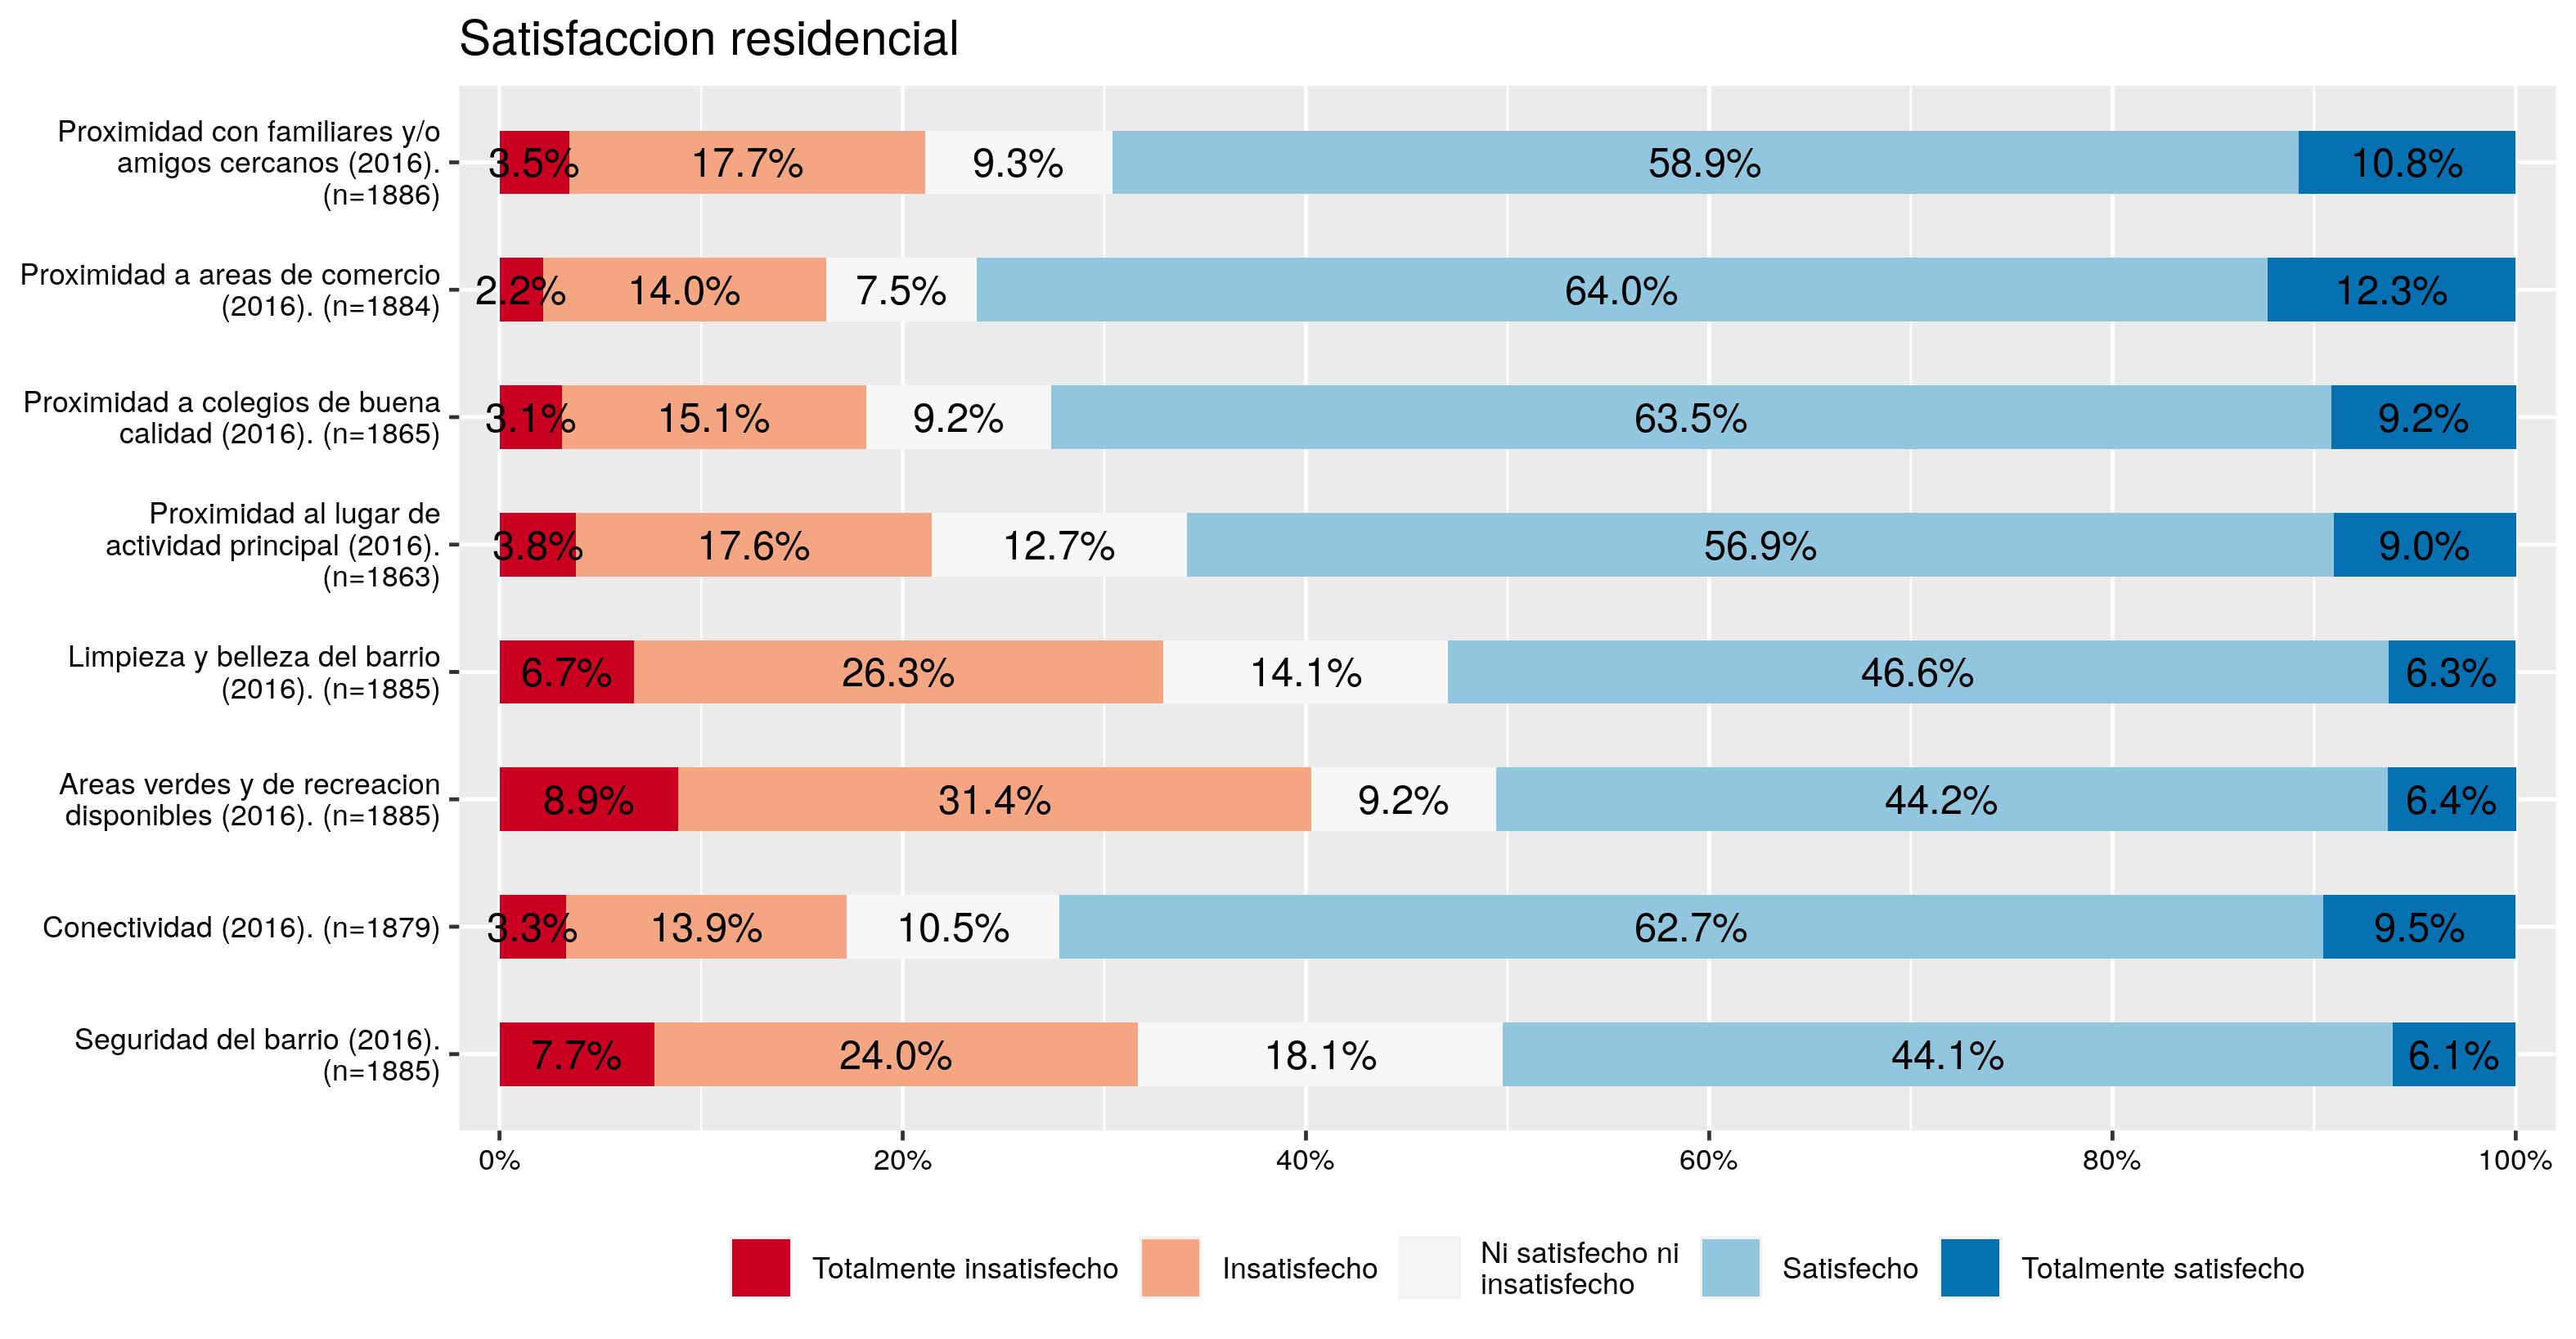
\includegraphics[width=1\linewidth,height=1\textheight]{output/graphs/satisfaccion-residencial} 

}

\caption{Satisfacción con el barrio.}\label{fig:satisfaccion-residencial}
\end{figure}

\begin{figure}[H]

{\centering 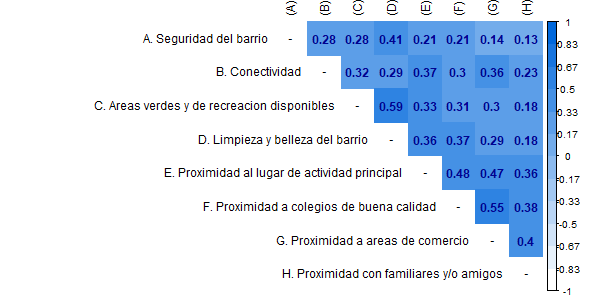
\includegraphics[width=1\linewidth,height=1\textheight]{output/graphs/satisfaccion-residencial_cor} 

}

\caption{Asociación indicadores satisfacción residencial.}\label{fig:satisfaccion-residencial-cor}
\end{figure}

Para la dimensión de cohesión territorial se realizó un único análisis factorial exploratorio. Como observamos en la Tabla \ref{tab:cohesion-territorial-fa}, en la segunda columna se presenta un factor que incluye los items referidos a la cohesión barrial, en la tercera columna se presenta un segundo factor asociado a la sociabilidad barrial y la confianza en vecinos y finalmente se presenta un tercer factor que incluye los items de satisfacción residencial. En cuanto a la varianza asociada a cada uno de estos factores, el primero de ellos representa el 15\% de la varianza, el segundo un 14\% de la varianza y el tercero un 13\% de la varianza. Por lo tanto, se propone utilizar un índice que incluya los cuatro items de cohesión barrial.

\begin{longtable}[]{@{}l@{}}
\caption{\label{tab:cohesion-territorial-fa}Dimensiones de cohesión territorial.}\tabularnewline
\toprule
\endhead

\includegraphics[width=8.33333in,height=\textheight]{output/tables/cohesion_territorial_fa.png} \\
\bottomrule
\end{longtable}

\hypertarget{resumen-de-la-propuesta-de-mediciuxf3n-de-la-cohesiuxf3n-social}{%
\section{Resumen de la propuesta de medición de la cohesión social}\label{resumen-de-la-propuesta-de-mediciuxf3n-de-la-cohesiuxf3n-social}}

A partir de los criterios propuestos y de los análisis realizados, proponemos utilizar el siguiente conjunto de indicadores para cada una de las subdimensiones, los que se muestran en la Tabla \ref{tab:descriptivos-cohesion}.

\label{tab:descriptivos-cohesion}Descriptivos medición de cohesión social.

Subdimensión

Indicadores

Min - max

Mean (sd)

Lazos

Cantidad de personas que se conocen con diferentes ocupaciones (2016)

1 - 5

3.941 (0.949)

Confianza interpersonal

Se puede confiar en la mayoria de las personas (2016).

1 - 3

1.314 (0.529)

La mayoria de las personas tratan de ayudar a las demas (2016).

Reconocimiento y respeto de la diversidad

Grado de confianza con personas homosexuales (2016).

1 - 5

2.752 (1.059)

Grado de confianza con personas mapuche (2016).

Grado de confianza con personas inmigrantes (2016).

Identificación con el país

Me siento orgulloso de ser chileno (2016).

4.245 (0.671)

Me identifico con Chile (2016).

Percepción de justicia

En Chile las personas son recompensadas por sus esfuerzos (2016).

2.67 (0.977)

En Chile las personas son recompensadas por su inteligencia (2016).

Confianza institucional

Confianza en el gobierno (2016).

1.799 (0.786)

Confianza en el presidente/a de la republica (2016).

Confianza en los partidos politicos (2016).

Solidaridad

Ha donado dinero a una obra social o de caridad (2016).

1 - 3

2.169 (0.591)

Ha prestado una suma de dinero de \$10.000.- o mas (2016).

Ha conversado con una persona en problemas o deprimida (2016).

Ha ayudado a alguien a conseguir trabajo (2016).

Participación cívica

Firmado una carta o peticion apoyando una causa (2016).

1 - 4.75

1.475 (0.657)

Asistido a una marcha o manifestacion pacifica (2016).

Participado en una huelga (2016).

Usado las redes sociales para expresar su opinion en temas publicos (2016).

Cohesión territorial

Este barrio es ideal para mi (2016).

1 - 5

3.625 (0.839)

Me siento integrado/a en este barrio (2016).

Me identifico con la gente de este barrio (2016).

Este barrio es parte de mi (2016).

Como una forma de evaluar la calidad de esta propuesta, en la Figura \ref{fig:cohesion-social-cor} se presenta la asociación entre las distintas subdimensiones de la cohesión social y, finalmente, en la Tabla \ref{tab:cohesion-social-fa} se presenta un análisis factorial exploratorio estimado entre las distintas subdimensiones, para evaluar si estas se ajustan con la propuesta de la CEPAL.

\begin{figure}[H]

{\centering 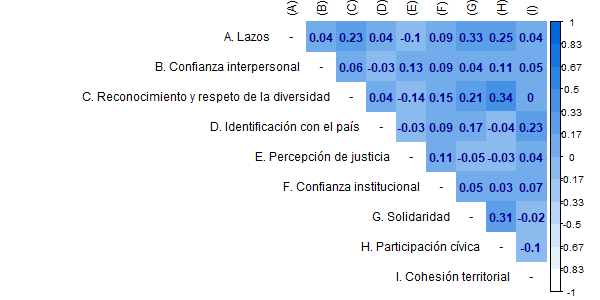
\includegraphics[width=1\linewidth,height=1\textheight]{output/graphs/cohesion_social_cor} 

}

\caption{Asociación de las subdimensiones de cohesión social.}\label{fig:cohesion-social-cor}
\end{figure}

\begin{longtable}[]{@{}l@{}}
\caption{\label{tab:cohesion-social-fa}Dimensiones de cohesión territorial.}\tabularnewline
\toprule
\endhead

\includegraphics[width=8.33333in,height=\textheight]{output/tables/cohesion_social_fa.png} \\
\bottomrule
\end{longtable}

\hypertarget{capuxedtulo-ii}{%
\chapter{Capítulo II ---}\label{capuxedtulo-ii}}

\hypertarget{capuxedtulo-iii}{%
\chapter{Capítulo III ---}\label{capuxedtulo-iii}}

\hypertarget{bibliografuxeda}{%
\chapter*{Bibliografía}\label{bibliografuxeda}}
\addcontentsline{toc}{chapter}{Bibliografía}

\hypertarget{refs}{}
\begin{CSLReferences}{1}{0}
\leavevmode\vadjust pre{\hypertarget{ref-cepal_cohesion_2021}{}}%
CEPAL. (2021). \emph{Cohesión social y desarrollo social inclusivo en {América Latina}. {Una} propuesta normativa para una era de incertidumbres}.

\leavevmode\vadjust pre{\hypertarget{ref-coes_radiografia_2019}{}}%
COES. (2019). \emph{Radiografía del cambio social. {Análisis} de {Resultados Longitudinales} 2016-2018}.

\leavevmode\vadjust pre{\hypertarget{ref-schiefer_essentials_2016}{}}%
Schiefer, D., \& Noll, J. van der. (2016). The {Essentials} of {Social Cohesion}: {A Literature Review}. \emph{Social Indicators Research}, 1--25. \url{https://doi.org/10.1007/s11205-016-1314-5}

\leavevmode\vadjust pre{\hypertarget{ref-valenzuela_vinculos_2008}{}}%
Valenzuela, E., Schwartzman, S., Valenzuela, S., Scully, T., Somma, N., \& Biehl, A. (2008). \emph{{Vínculos, creencias e ilusiones. La cohesión social de los latinoamericanos \textendash{} Cieplan}} (Uqbar).

\end{CSLReferences}

\end{document}
